\documentclass[12pt,openany,final]{book}

%------------------------------------------------------------------------------
% Geometry (locked margins per dissertation requirements)
%------------------------------------------------------------------------------
\usepackage[letterpaper,margin=1in,footskip=0.25in]{geometry}

%------------------------------------------------------------------------------
% Fonts & encoding
%------------------------------------------------------------------------------
\usepackage[T1]{fontenc}
\usepackage[utf8]{inputenc}
\renewcommand*\familydefault{\rmdefault} % use default CM Roman cleanly

%------------------------------------------------------------------------------
% Microtypography for better spacing/justification
%------------------------------------------------------------------------------
%\usepackage[final,tracking=true,expansion=true,protrusion=true]{microtype}
\usepackage[final,tracking=true,expansion=false,protrusion=true]{microtype}
\microtypesetup{stretch=10,shrink=10,step=1}

%------------------------------------------------------------------------------
% General packages
%------------------------------------------------------------------------------
\usepackage[final]{changes}
\usepackage{lipsum}
\usepackage[nottoc]{tocbibind}
\usepackage{flafter}
\usepackage{floatrow}
\usepackage{pdflscape}
\usepackage{fancyhdr}

\pagestyle{fancy}

\newcommand{\rotatenextpagenumber}{%
  \AddToShipoutPictureFG*{%
    \AtPageCenter{%
      \makebox[0pt][l]{%
        \hspace*{\dimexpr 0.5\paperwidth - 1in\relax}%
        \rotatebox{90}{\thepage}%
      }%
    }%
  }%
}



\fancypagestyle{landscapepage}{%
  \fancyhf{}
  % \fancyfoot[C]{\thepage}
  \renewcommand{\headrulewidth}{0pt}
  \renewcommand{\footrulewidth}{0pt}
    }%
  



\newenvironment{swaplandscape}
  {%
  \begin{landscape}
    \pagestyle{landscapepage}
   \rotatenextpagenumber 
  }
  {%
  \end{landscape}
  \pagestyle{fancy}
  }



\usepackage{float}
\floatstyle{plaintop}
\restylefloat{table}
\usepackage[section]{placeins}
\makeatletter
\let\oldsubsection\subsection
\renewcommand{\subsection}{%
  \FloatBarrier
  \oldsubsection
}
\let\oldsubsubsection\subsubsection
\renewcommand{\subsubsection}{%
  \FloatBarrier
  \oldsubsubsection
}
\makeatother
\usepackage{siunitx}
\usepackage{graphicx}
\graphicspath{{figures/}}% input figure files
\usepackage{dcolumn}% Align table columns on decimal point
\usepackage{appendix}
\usepackage{amsmath}
\usepackage{longtable}
\usepackage{amssymb}
\usepackage{cases}
\usepackage{calc}
\usepackage{color}
\usepackage{rotating}
\usepackage{enumitem}
\usepackage{soul}
\usepackage{indentfirst}
\usepackage{hyphenat}
\usepackage{xspace}
\usepackage{subcaption}
\usepackage{booktabs}
\usepackage{multirow}
\usepackage{tabularx}
\usepackage{xtab}
\newcolumntype{Y}{>{\centering\arraybackslash}X}
\usepackage{lineno}
\usepackage{setspace}
\usepackage{titlesec}
\usepackage{hyperref}
\usepackage[superscript]{cite}
\usepackage{pdfpages}


\usepackage{xcolor}
\usepackage{caption}

\captionsetup{
    labelfont={color=black!75},
    textfont={color=black!75}
}
%------------------------------------------------------------------------------
% Title formatting
%------------------------------------------------------------------------------
\titleformat{\chapter}
  {\normalfont\normalsize\bfseries\centering}{\thechapter}{1em}{}
\titleformat{\section}
  {\normalfont\normalsize\bfseries}{\thesection}{1em}{}
\titleformat{\subsection}
  {\normalfont\normalsize}{\thesubsection}{1em}{}
\titleformat{\subsubsection}
  {\normalfont\normalsize\itshape}{\thesubsubsection}{1em}{}
\titleformat{\paragraph}[runin]
  {\normalfont\normalsize\bfseries\itshape}{\theparagraph}{1em}{}
\titleformat{\subparagraph}[runin]
  {\normalfont\normalsize\itshape}{\thesubparagraph}{1em}{}

% Chapter spacing
\titlespacing*{\chapter}{0pt}{0.5in}{0.25in}
\titlespacing*{\section}{0pt}{0pt}{0pt}
\titlespacing*{\subsection}{0pt}{0pt}{0pt}
\titlespacing*{\subsubsection}{0pt}{0pt}{0pt}
\setcounter{secnumdepth}{3}

%------------------------------------------------------------------------------
% Spacing and float tuning
%------------------------------------------------------------------------------
% \onehalfspacing              % 1.5 line spacing, common dissertation req.
\setlength{\parskip}{0pt}    % no vertical gap between paragraphs
\setlength{\parindent}{0.5in} % indent new paragraphs
% \raggedbottom                % prevent vertical stretch across pages
\flushbottom

% Float parameters (reduce white space holes)
\renewcommand{\topfraction}{0.97}
\renewcommand{\bottomfraction}{0.97}
\renewcommand{\textfraction}{0}   % allow pages with very little text
\renewcommand{\floatpagefraction}{1} % effectively disable float-only pages
\setcounter{topnumber}{4}
\setcounter{bottomnumber}{3}
\setcounter{totalnumber}{6}

% Tighter spacing around floats
\setlength{\floatsep}{3pt plus 0pt minus 0pt}      % between floats
\setlength{\textfloatsep}{3pt plus 0pt minus 0pt}  % float <-> text
\setlength{\intextsep}{2pt plus 0pt minus 0pt}     % in-text float <-> text

% Keep floats from sticking to top/bottom with giant gaps
\makeatletter
\setlength{\@fptop}{0pt}
\setlength{\@fpbot}{0pt plus 1fil}
\makeatother

% Widow/orphan penalties
\clubpenalty=3000
\widowpenalty=3000
\displaywidowpenalty=3000

% Line-breaking tolerance
\tolerance=2000
\emergencystretch=2em
\hyphenpenalty=200
\exhyphenpenalty=50


%------------------------------------------------------------------------------
% Hyperref setup (black links for print compliance)
%------------------------------------------------------------------------------
\hypersetup{
    colorlinks,
    citecolor=black,
    filecolor=black,
    linkcolor=black,
    urlcolor=black
}
%------------------------------------------------------------------------------
% TOC / LOF / LOT formatting
%------------------------------------------------------------------------------
\usepackage[figurewithin=none,tablewithin=none]{caption}
\usepackage[titles]{tocloft}

\setlength\cftbeforechapskip{\baselineskip}
\setlength\cftbeforefigskip{\baselineskip} % one single-spaced line between figures
\setlength\cftbeforetabskip{\baselineskip} % one single-spaced line between tables
\setlength\cftfigindent{0in}
\setlength\cfttabindent{0in}
\cftsetpnumwidth{0.5in}
\cftsetrmarg{0.5in}

% No dots
\renewcommand{\cftdot}{}

% Chapter fonts
\renewcommand{\cftchapfont}{\normalsize}
\renewcommand{\cftchappagefont}{\normalsize}

%------------------------------------------------------------------------------
% TOC hierarchy + spacing
%------------------------------------------------------------------------------

% Level 1: Chapter — flush with margin
\setlength{\cftchapindent}{0in}
\setlength{\cftchapnumwidth}{5em}          % room for "Chapter 10"
\renewcommand{\cftchappresnum}{Chapter~}
\renewcommand{\cftchapaftersnum}{\ }

% Level 2: Section — 0.5" indent
\setlength{\cftsecindent}{0.5in}
\setlength{\cftsecnumwidth}{1.8em}
\renewcommand{\cftsecaftersnum}{\ }

% Level 3: Subsection — 1.0" indent
\setlength{\cftsubsecindent}{1.0in}
\setlength{\cftsubsecnumwidth}{2.5em}
\renewcommand{\cftsubsecaftersnum}{\ }

%------------------------------------------------------------------------------
% LIST OF TABLES (LOT)
% "Table #" flush left, caption starts at 0.75" (or 1")
%------------------------------------------------------------------------------

\renewcommand{\cfttabpresnum}{Table~}
\renewcommand{\cfttabaftersnum}{\ }

\setlength{\cfttabindent}{0in}      % "Table #" at left margin
\setlength{\cfttabnumwidth}{5em} % caption block starts at 0.75"
% (use 1in instead if they insist on 1")

%------------------------------------------------------------------------------
% LIST OF FIGURES (LOF)
% "Figure #" flush left, caption starts at 0.75" (or 1")
%------------------------------------------------------------------------------

\renewcommand{\cftfigpresnum}{Figure~}
\renewcommand{\cftfigaftersnum}{\ }

\setlength{\cftfigindent}{0in}      % "Figure #" at left margin
\setlength{\cftfignumwidth}{5em} % caption block starts at 0.75"
% (again, change to 1in if they want 1")



%------------------------------------------------------------------------------
% URL formatting
%------------------------------------------------------------------------------
\usepackage{url}
\urlstyle{same}

%------------------------------------------------------------------------------
% Custom macros
%------------------------------------------------------------------------------
\newcommand{\norm}[1]{\left\lVert#1\right\rVert}
\newcommand{\cmpersec}{cm/s~}
\newcommand{\etal}{\textit{et al.}}
\newcommand{\PM}{$\pm$~}
\newcommand{\invnm}{$\text{\si{\nm}}^{-1}$~}
\newcommand{\nmeter}{\si{\nm}~}
\newcommand{\tbxmulticol}[3]
    {\multicolumn{#1}
                 {>{\centering\hsize=\dimexpr#1\hsize+#1\tabcolsep+\arrayrulewidth\relax}#2}
                 {#3}}
\newcommand{\ra}[1]{\renewcommand{\arraystretch}{#1}}
\renewcommand{\arraystretch}{1.8}
\newcommand{\sigmaij}{$\sigma_{ij}$}
\newcommand{\epsilonij}{$\epsilon_{ij}$}
\newcommand{\db}{$\text{D}_\text{B}$}
\newcommand{\dhh}{$\text{D}_\text{hh}$}
\newcommand{\dc}{$\text{2D}_\text{C}$}
\newcommand{\al}{$\text{A}_{\text{L}}$}
\newcommand{\Vl}{$\text{V}_{\text{L}}$}
\newcommand{\Vh}{$\text{V}_{\text{H}}$}
\newcommand{\Vc}{$\text{V}_{\text{C}}$}
\newcommand{\vl}{$\text{V}_{\text{L}}$}
\newcommand{\vh}{$\text{V}_{\text{H}}$}
\newcommand{\vc}{$\text{V}_{\text{C}}$}
\newcommand{\sig}{$\sigma$}
\newcommand{\eps}{$\epsilon$}
\newcommand{\na}{Na\textsuperscript{+}}
\newcommand{\li}{Li\textsuperscript{+}}
\newcommand{\mg}{Mg\textsuperscript{2+}}
\newcommand{\cl}{Cl\textsuperscript{-}}
\newcommand{\mgcl}{MgCl\textsubscript{2}}
\newcommand{\nacl}{NaCl}
\newcommand{\licl}{LiCl}
\newcommand{\mbnbfix}{MB-NB-fix~}
\newcommand{\mbnbfixmicro}{Grotz \etal~}
\newcommand{\nambnbfix}{Na\textsuperscript{+}--Saunders \etal}
\newcommand{\limbnbfix}{Li\textsuperscript{+}--Joung and Cheatham}
\newcommand{\mgmbnbfix}{Mg\textsuperscript{2+}--Li \etal}
\newcommand{\mgmicro}{Mg\textsuperscript{2+}--Grotz \etal}
\newcommand{\mglbrules}{Mg\textsuperscript{2+}--Li \etal}
\newcommand{\TODO}{\hl{TODO}~}
\newcommand{\about}{$\sim$}
\newcommand{\aangstroms}{{\aa}ngstr{\"o}ms}
\newcommand{\aangstrom}{{\aa}ngstr{\"o}m}
\newenvironment{hle}{\color{red}}

\newcommand{\beginsupplemental}{%
    \setcounter{table}{0}
    \renewcommand{\thetable}{S\arabic{table}}%
    \setcounter{figure}{0}
    \renewcommand{\thefigure}{S\arabic{figure}}%
}

\renewcommand{\bibname}{References}
\renewcommand{\contentsname}{Table of Contents}

\author{Matthew Saunders}
\begin{document}

\pagestyle{plain}
%\maketitle
\pagenumbering{roman}
\begin{titlepage}
\begin{centering}

~\\[1in]
Parameterizing Ion–Lipid Interactions from Local Clusters to \\~\\Reproduce Experimental Bulk Properties of Lipid Bilayers
~\\[3\baselineskip]
by
~\\[3\baselineskip]
Matthew W. Saunders
~\\[4\baselineskip]
A thesis submitted in partial fulfillment\\
of the requirements for the degree of\\
Doctor of Philosophy\\
Department of Molecular Biosciences\\
College of Arts and Sciences\\
University of South Florida
~\\[3\baselineskip]
Co-Major Professor: Sameer Varma, Ph.D.\\
Co-Major Professor: Sagar Pandit, Ph.D.\\
Jianjun Pan, Ph.D.\\
Libin Ye, Ph.D.\\
Stanley Stevens, Ph.D.
~\\[2\baselineskip]
Date of Approval:~\\
October 1, 2025 
~\\[3\baselineskip]
Keywords: Molecular Dynamics, Zwitterion, Ion Adsorption, Force-Field, Phospholipid\\
~\\
Copyright \textsuperscript\textcopyright~2025, Matthew W. Saunders\\

\end{centering}
\end{titlepage}
% \begin{frontmatter}
\tableofcontents
\listoftables
\listoffigures
\bibliographystyle{elsarticle-num}
\doublespacing
\clearpage
\chapter*{Abstract}
\addcontentsline{toc}{chapter}{Abstract}
Phospholipids are the main component of cell membranes, providing a delimiting boundary for cells from their environments or from their organelles from the cytosol. 
This compartmentalization allows cells to maintain quite different solutions within their cells and organelles, including different mixtures dissolved ions. 
Consequently, these membranes are constantly flanked by complex mixtures of salts at varied concentrations. To study membrane structure, one cannot neglect the 
contribution of the salts in the local solution. Ions perturb bilayer structure via specific interaction with the phospholipids, primarily with the headgroups. 
Experimental studies of these systems are somewhat at odds --- scattering experiments with different salts and zwitterionic lipids report no significant change in bilayer structure with 
concentrations as large as 1 M for monovalent ions, and at physiologically relevant concentrations for \mgcl{}. Groups have reported via headgroup NMR that the headgroup tilt angle 
is modulated by ion interaction, and thus there must be some adsorption that occurs. Simulations also report thickening of lipid bilayers by ions. 
Here this discrepancy is addressed by the application of a novel optimization procedure using \emph{ab initio} substitution energies and associated binding geometries of ions from water to lipid headgroups
as targets for model parameter optimization. We apply parameters to replace Lennard–Jones mixing rules. Simulations of \nacl{} are much more in line with experiments than the mixing rule results. 
\mgcl{} proves more complicated, and herein we propose and characterize two sets of parameters that give different results. We characterize the adsorption modes that \na{}, \li{}, \mg{}, and \cl{} take
when adsorbed to a bilayer of 1-palmitoyl-2-oleoyl-sn-glycero-3-phosphatidylcholine (POPC), and characterize how these binding modes result in perturbation of the lipid bilayer structure. Experiments 
are needed to validate the \mg{} parameters, and several validation targets are provided within. 
% \end{frontmatter}
\clearpage
\pagenumbering{arabic}
\chapter[Introduction]{Introduction\footnote{Portions reprinted with permission from Matthew Saunders, Vered Wineman-Fisher, and Eric Jakobsson, \textit{High-Dimensional Parameter Search Method to Determine Force Field Mixing Terms in Molecular Simulations}, 
\textit{Langmuir}, American Chemical Society, March 1, 2022., from Matthew Saunders, Abibat Adekeye-Olowofela, and Sabrina Downing, \textit{Adsorption Modes of Na\textsuperscript{+}, Li\textsuperscript{+}, and Mg\textsuperscript{2+} to a Model Zwitterionic Lipid Bilayer}, 
\textit{Langmuir}, American Chemical Society, December 1, 2024., and from Matthew Saunders, Sagar Pandit, and Sameer Varma, Alteration of Lipid Bilayer Structure by \mg{}, \textit{Langmuir}, American Chemical Society, manuscript in review, 2025. See appendix~\ref{app:permissions} for reuse permissions and author contributions.}}
 \graphicspath{{CH1/figures/}}
\section{Phospholipid bilayers}
Phospholipid bilayers are the primary component of the major delimiting boundary between cells and their environment.
These membranes are not static walls so much as liquid-crystalline, rapidly exploring their conformational
space and adjusting to the external and internal cellular environment. Cells, through the 
diversity of chemistry of headgroups and acyl-chain selections, tailor the dynamic structure of their membrane to further
adapt to the environment around them. 
Understanding the way that individual lipid species contribute to the structure of a lipid bilayer is critical to understand
why a cell might choose one lipid or another in their cell membrane. Additionally, because these lipids are exposed to complex
mixtures of ions on either side of the membrane, the interactions with ions in solution cannot be ignored when discussing the bilayer structure. 
Experimentally observed ion behavior at an interface in solution has been explained using a mean-field model~\cite{israelachvilli:2011:intermol}.
However, this ignores specific chemical interactions between lipid molecules and the ions in the solvent, that are critical for understanding
the effect of changing headgroup species in a membrane. 
Computational models can enable researchers to observe the specific ion-lipid interactions are critical for understanding of 
why cells might choose certain lipids to manipulate their membrane structure under varied ion mixtures in their environment. Furthermore, this 
changing membrane structure also affects the behavior of membrane protiens embedded in the bilayer. Thus, this manipulation of the lipid mixture
presents itself as an important regulatory mechanism for cells.
\subsection{Effects of ions on lipid bilayer structure}
The effects of dissolved salts on bilayers has been studied with varied methodologies. 
One of the more commonly applied methods of study
is small-angle x-ray scattering (SAXS) and neutron scattering (SANS). 
Lipid bilayers are smectic crystals, and thus give scattering
patterns that look like concentric rings in reciprocal space -- these circles are the bilayer form-factor~\cite{nagle:2000}. This form-factor
is the reciprocal-space structure of the bilayer. 
However, a direct Fourier inversion cannot be performed due to the loss of phase information.
In order to produce the appropriate density distribution, one can approximate the number density of bilayer parts as gaussian functions, and 
compute the appropriate scattering density from that~\cite{nagle:2000,fogarty:2015}. This can then be transformed via a cosine transform
into a form-factor. The gaussians are then adjusted
until the resulting continuous form-factor fits the data from the experiment~\cite{nagle:2000,fogarty:2015}.

SAXS and SANS experiments to study lipid bilayers in the presence of dissolved salt have reported
largely that salts do not have a significant affect on zwitterionic lipid bilayer 
structure~\cite{pabst:2007,petrache:2006:swelling,uhrikova:2008,kurakin:2021:effect}.
Petrache \etal{} observed that with multilamellar vesicles of 1,2-dilauroyl-sn-glycero-3-sn-glycero-phosphatidylcholine 
as well as other lipids in KCl and BrCl salt solutions, 
and reported that while small changes can be seen in the
X-ray scattering form-factor due to the 
salts, 
the fitted electron density profiles are essentially identical for
systems with and without 
salt~\cite{petrache:2006:swelling}. 
Similarly, Pabst \etal{} found no significant change in bilayer structure 
for POPC bilayers in NaCl salt at or below 1 M concentration~\cite{pabst:2007}.
Furthermore, Uhrikova \etal{} reported small structural changes using small angle neutron scattering
(SANS) experiments on 1,2-dipalmitoyl-sn-glycero-3-phosphatidylcholine 
vesicles interacting with CaCl$_{2}$~\cite{uhrikova:2008}. 
Taken together, these results point to a general discrepancy between structural data 
from MD simulations and scattering experiments.
Kurakin \etal{} reported that in bilayers of POPC, divalent cations such as \mg and Ca\textsuperscript{2+} also cause
no major alteration in lipid bilayer structure at biologically relevant concentrations of \mg~\cite{kurakin:2021:effect}.

While SAXS and SANS methods do not see a change in the overall structure of lipid bilayers methods like NMR of deuterated headgroup carbons 
indicate changes in the headgroup tilt angle of neutral lipids in salt solutions, suggesting some interaction~\cite{akutsu:1981,seelig:1987}. 
This would indicate that there should be ion binding or adsorption to the bilayer interface, that is not visible in the SAXS or SANS form-factor but 
could be observed through other methods. Additionally, AFM measurements can observe some changes in the organization of lipids in a 
gel phase bilayer in the presence of salts, again indicating some interaction 
and adsorption while the area-per-lipid of the bilayer remains largely unchanged~\cite{ferber:2011:direct}.

Molecular simulations can gather atomistic detail of systems, and are often useful for systems like lipid bilayers. Simulations of bilayers
in salt using many different simulation models 
have reported that there is significant ion binding to the lipid bilayer, and subsequent 
thickening of the lipid bilayer when compared to the structure 
of a bilayer in pure 
water~\cite{Bockmann:2003,cordomi:2008,gurtovenko:2008,Cordomi:2009,jurkiewicz:2012,pandit:2008:simulationtextbook,kruczek:2017,kruczek:2019,saunders:2019}.
This persistent discrepancy between the large-scale structural changes predicted by 
simulations and the subtle rearrangements observed experimentally highlights the need for improved 
ion–lipid interaction models that better capture experimental behavior. 
In the following chapters, this problem is addressed through the development of a generalizable 
method for selecting molecular simulation parameters to reproduce target experimental data, and through 
the application of this method to refine lipid–ion interaction models across a range of salt solutions. 
The remainder of this introduction outlines the simulation and analysis methods employed throughout this work, 
while the subsequent chapters present the specific results obtained.


\section{Molecular Simulations}
\subsection{Classical Molecular Dynamics}
Molecular Dynamics utilizes computers to simulate systems of molecules in order to study how structure changes
with time, and the specific ways that different atomic and molecular species interact. This is done
by first creating a model for the Hamiltonian of the system -- a "force-field". This consists firstly of the terms for how atoms
bond to each other, how these bonds move and stretch, and how they rotate around each other; classical models
usually use harmonic potentials for bond and angle stretching and bending, and dihedrals 
are described using periodic functions~\cite{gromacsmanual}.
In addition to the bonded terms, we have the non-bonded terms — energy from 
electrostatic interactions, typically described by Coulomb's law, and dispersion 
interactions (Van der Waals, or VdW) which arise from instantaneous dipole–induced dipole effects~\cite{gromacsmanual}. These are 
most often modeled using a Lennard–Jones (LJ) potential~\cite{Jones:1924,gromacsmanual}, though other forms are 
also common, such as the Buckingham (exp–6) potential~\cite{Buckingham:1938,gromacsmanual}, which replaces the steep 
\(r^{-12}\) repulsive wall with a short-range exponential. In addition to these two, there are many other
functional forms used to describe VdW and dispersion interactions, but they are far less common. An example of this Hamiltonian
can be seen here:
\begin{align}
E_{\mathrm{total}} &= E_{\mathrm{bonded}} + E_{\mathrm{nonbonded}} \\
E_{\mathrm{bonded}} &= \sum_{\text{bonds}} k_r (r - r_0)^2
+ \sum_{\text{angles}} k_\theta (\theta - \theta_0)^2
+ \sum_{\text{dihedrals}} V_n \left[ 1 + \cos\left( n\phi - \gamma \right) \right] \\
E_{\mathrm{nonbonded}} &= \sum_{i<j} \left[ 4\epsilon_{ij} \left( \left( \frac{\sigma_{ij}}{r_{ij}} \right)^{12}
- \left( \frac{\sigma_{ij}}{r_{ij}} \right)^{6} \right)
+ \frac{q_i q_j}{4\pi\epsilon_0 r_{ij}} \right]
\end{align}

By using this set of terms one can compute the potential energy of a particular configuration of particles. 
The forces obtained from the potential energy are used in Newton’s equations of motion, 
which are numerically integrated — most often with algorithms such as the velocity-Verlet method — 
to update positions and velocities at each time step~\cite{gromacsmanual}.
The energy of the new configuration
can be computed, and the simulation continues. Thus, the careful development and improvement of a force-field is critical to 
reproduce valid results that can help us understand what is seen in experiments.

\subsection{Mixing rules, and NB-fix}
Focusing in particular on the non-bonded terms of the hamiltonian, and specifically the Lennard-Jones (LJ) function, we note that there are two
free parameters \sigmaij{} and \epsilonij{} between a particular pair of particles $i$ and $j$:
\begin{equation}
E_{\mathrm{LJ}_{ij}} = 4\epsilon_{ij} \left( \left( \frac{\sigma_{ij}}{r_{ij}} \right)^{12}
- \left( \frac{\sigma_{ij}}{r_{ij}} \right)^{6} \right)
\end{equation}
Where $r_{ij}$ is the distance between the two particles, \sigmaij{} is the characteristic distance of the Van der Waals interaction between the two species,
and \epsilonij{} is the characteristic energy of the interaction.
These parameters are generally determined for a particular species for the case of the self-interaction, or $\sigma_{ii}$ and $\epsilon_{ii}$.
In this case, they represent roughly the atomic radius, and the ``stickyness'' of the particle. These can then be combined with the 
$\sigma_{jj}$ and $\epsilon_{jj}$ from another species by using what are called mixing rules, developed to 
model the interaction radii and energy well-depth for interacting species~\cite{lorentz:1881,berthelot:1898}.
The Lorentz rule for computing the \sigmaij{} is simply the arithmetic mean of the self terms from the two species, and 
the Berthelot rule for computing the \epsilonij{} is the geometric mean of the self terms.
Modern works have often reported that these mixing rules fail
or behave unpredicatbly for more complicated species than the noble gases~\cite{fyta:2012,boda:2008:effects},
and abandonment of the mixing rules for specifically selected cross-terms can be beneficial to improving
force-fields~\cite{baker:2010:accurate,yoo:2012:improved,fyta:2012:ionic,mamatkulov:2013:force,venable:2013,
savelyev:2014:balancing,li:2015:representation,savelyev:2015:competition,jing:2017:study,reif:2017,wineman:2019}. This 
kind of correction is often called a "non-bonded fix" or NB-fix, which is a correction to the cross-terms of the species of interest 
in order to improve the reproduction of some experimental result.
In this dissertation, I expand on the idea of a NB-fix method to improve the modeling of the interactions of ions and phospholipid species.
However, the method proposed and characterize is general, and can be applied to other chemically diverse systems of interest.

\subsubsection{MD methods utilized in this dissertation}
In the following dissertation, unless otherwise specified, I perform all molecular dynamics simulations with the GROMACS software 
package~\cite{abraham:2015,pall:2014,van:2005,lindahl:2001,berendsen:1995,gromacs}.
I use the SPC/E model for all waters~\cite{spce}, and I describe lipid interactions
with the gromos43A1-S3 parameter set developed by our group in previous work~\cite{chiu:2009}.
System temperature is maintained at 300~K using the Nos\`e--Hoover thermostat
with a coupling constant of 0.5~ps~\cite{nose:1983}, and pressure is maintained
at 1~atm with the Parrinello--Rahman semiisotropic barostat using a coupling constant of 1.5~ps~\cite{parrinello:1981}.
All bonds are constrained with the P--LINCS algorithm, which allows the use of a 4~fs integration timestep~\cite{lincs}.
Equations of motion are integrated with the Verlet scheme, and neighbor lists are updated every 2 steps.
Electrostatic interactions are treated with the particle--mesh Ewald (PME) method~\cite{essmann:1995},
using a real--space cutoff of 1.6~nm and reciprocal grids of either
$56 \times 56 \times 224$ or $52 \times 52 \times 240$ cells,
together with 4th order B--spline interpolation.
Van der Waals interactions are calculated with a single cutoff of 1.6~nm.
\subsubsection{Simulation system construction}
All simulations systems unless otherwise noted are constructed by first creating a leaflet of 100 POPC lipids arranged
on a $10 \times 10$ grid with sufficient spacing to avoid chain overlap.
This leaflet is then reflected along the $z$--axis to generate the second
leaflet, producing a bilayer of 200 lipids. A solvent block is added by
placing 60,000 water molecules on a three--dimensional grid with excess spacing,
and a subset of water molecules is randomly replaced with ions to achieve a
starting concentration of 200~mM (see Table~\ref{tabch3:ions}).

Energy minimization is performed using the steepest--descents algorithm with a
force tolerance of 50~kJ~mol$^{-1}$~nm$^{-1}$. Electrostatic interactions are
treated with the particle--mesh Ewald (PME) method~\cite{essmann:1995}, using a
real--space cutoff of 1.6~nm, reciprocal grid spacing of 0.12~nm$^{-1}$, and
6th order B--spline interpolation. Van der Waals interactions are calculated
with a single cutoff of 1.6~nm. Neighbor searching is performed every 2 steps.

Following energy minimization, I relax the system with a constant--pressure
simulation at 290~K for 200~ps. Simulation systems are then annealled by heating the system above the
simulation run temperature, and then cooling down to the production temperature following the
specific procedure outlined in each following chapter.

\subsection{\emph{Ab initio} calculations and Density Functional Theory}
Classical force-fields are effective for simulating large-systems of particles where an explicit description of 
the electronic behavior is not critical to the understanding of how the particles behave -- while this is a major 
approximation, it turns out to often be useful in studying biological structures like lipid membranes~\cite{berkowitz:2019}.
However, when preparing these classical models, we need to refer to more complicated theory in the form 
of quantum mechanical calculations to set terms like the 
charge per particle in a molecule and to compare to the molecular structure predicted by our bonded-parameters.
\emph{Ab initio} quantum mechanical calculations include chemistry by explicitly describing the behavior of electrons to varied 
levels of accuracy depending on the kind of functional form used, and then the basis vectors used to describe the space.
Pertubation theory methods include electron correlation, which can be useful for assigning electrons to parts of a molecule. 
However, these methods quickly become expensive for systems with many electrons. Density functional theory, which treats the electrons 
with a mean-field approximation is often more computationally efficient and can thus be applied to larger systems.

\emph{Ab initio} methods are used in the works included in this dissertation to generate target data for 
model parameter optimization from geometry
optimizations and substitution energies of small ion–ligand clusters
using density functional theory (DFT) as implemented in
FHI-aims~\cite{fhiaims}. Initial cluster geometries are produced with
the molecular mechanics force field developed in our previous
work~\cite{kruczek:2017,saunders:2019} and then optimized at the DFT
level. I use the PBE0 functional~\cite{perdew:1996:generalized,adamo:1999:toward}
with Tkatchenko–Scheffler dispersion corrections~\cite{tkatchenko:2009},
a combination that has been benchmarked for ion–ligand clusters and shown
to reproduce experimental data and high-level quantum methods across a
range of chemistries~\cite{wineman:2019,wineman:2020:transferable,wineman:2020:improved}.
Geometry optimizations are first performed with the ``light'' basis set
and then refined with the ``really tight'' basis set provided in
FHI-aims. Optimizations are converged to 0.005~eV/\AA{} in forces and
$10^{-6}$~eV in total energy.  

Energies of optimized clusters are then used to compute substitution
energies, defined as the energy of exchanging water molecules
with headgroup analog ligands. The specific cluster sets and substitution
energy targets used for parameterization are described in the relevant
chapters.

\section{Comparing Molecular Simulations with Experimental Results}
\subsection{SAXS (and SANS) -- and other properties obtained from density distributions}
In simulations, we can compute the number density histograms of the system components
directly from the trajectories, and thus the electron densities directly. Once we have the electron density of our system
per nanosecond, we determine the lipid bilayer centerpoint by locating the minimum at the center of the 
histogram. We symmetrize the histogram around the minimum at the center, and then take an average over many nanoseconds.
We subtract the bulk solvent value of the electron density from the average histogram, and then use a cosine transform
to obtain the bilayer SAXS form-factor. This can be compared with the experimental data directly.
We also use the electron density to directly obtain the peak-to-peak distance of the bilayer, \dhh{}, as one measure
of the bilayer thickness.
\subsection{Obtaining \db{} and \dc{}}
The number density histograms are also used to compute the various bilayer thicknesses via probability densities
of the various system components. We compute the bilayer thickness \db{} and \dc{} by compiuting probability densities
for the solvent, and the lipid acyl chains respectively. We determine the Gibbs' dividing surface of these by finding the point in the interfacial region
where the area above the histogram is equal to below -- the distance from this point to the bilayer center is used as the respective bilayer thickness.
These measures are visualized in figure~\ref{figch1:thicknesses}.
\begin{figure}[h!tb]
    \caption{ }
    \label{figch1:thicknesses}
    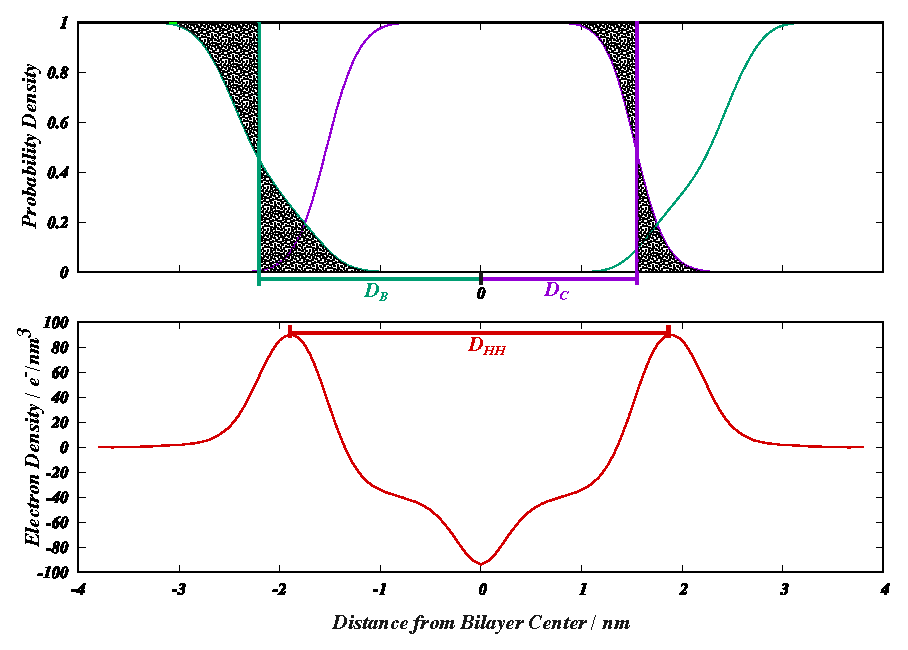
\includegraphics{Probabilitydens.eps}
\end{figure}
\subsection{Lipid component volumes}
Phospholipid headgroup and chain occupied volumes are computed using the method of Petrache \etal{} for computing the
volume of immiscible liquids~\cite{petrache:1997} using the number density histograms of the headgroups, acyl-chains, and solvent.
In the work outlined in this dissertation, we identify lipid chains are as starting 
at the first carbon attached to the lipid chain carbonyl oxygen, including the oxygen.
The atom groups not part of the lipid
chains are partitioned into the headgroup volume. 
The number--density of these component groups along with that of the solvent are taken 
and used to optimize the objective function:
\begin{equation}
    \label{eq:volumeobj}
    \Omega(v_i)=\sum^{\rho_s}_{z_j}(1-\sum^{N_{\text{Groups}}}_{i=1}{(\rho_i(z_j)v_i)^2})\text{,}
\end{equation}
In the equation above, $\rho_i(z_j)$ is the number density of the $i$ component in the
$z_j$ slice of the box and $v_i$ is the corresponding component volume. 
The component volumes are then multiplied by the corresponding
number of particles per molecule per group -- 32 for the chain
particles, and 20 for the headgroup. 
This gives us the total volume per molecule for each group, defined as \Vh{} and \Vc{}. These are then
added together to make the total \Vl{}.
\subsection{Deuterium Order parameters}
\subsubsection{Acyl-chain CD order parameters}

\subsubsection{D2O Water orientational order parameters}


\chapter[A High Dimensional Parameter Search Method to...]{A High Dimensional Parameter Search Method to Determine Force Field Mixing Terms in Molecular Simulations\footnote{
Portions reprinted with permission from Matthew Saunders, Vered Wineman-Fisher, and Eric Jakobsson, \textit{High-Dimensional Parameter Search Method to Determine Force Field Mixing Terms in Molecular Simulations}, 
\textit{Langmuir}, American Chemical Society, March 1, 2022. 
\textcopyright{} 2022 American Chemical Society. See appendix~\ref{app:permissions1} for reuse permissions and author contributions.
}}
\graphicspath{{CH2/figures/}}

\begingroup
\makeatletter
% Save originals
\let\origfigure\figure
\let\endorigfigure\endfigure
\let\origtable\table
\let\endorigtable\endtable

% Redefine environments so any optional argument is ignored and [H] is used
\renewenvironment{figure}[1][]{\origfigure[H]}{\endorigfigure}
\renewenvironment{table}[1][]{\origtable[H]}{\endorigtable}
\makeatother


\section{Abstract}
Molecular dynamics (MD) force fields for lipids and ions are typically developed independently of one another. 
In simulations consisting of both lipids and ions, 
lipid-ion interaction energies are estimated using a predefined 
set of mixing rules for Lennard-Jones (LJ) interactions. 
This, however, does not guarantee their reliability. 
In fact, compared to the quantum mechanical reference data, 
Lorentz-Berthelot mixing 
rules substantially underestimate binding energies of \na~ ions with small 
molecule analogues of lipid headgroups, yielding errors on the order of 80 and 130 kJ/mol, 
respectively for methyl acetate and diethyl phosphate. Previously, errors 
associated with mixing force fields have been reduced using approaches like `NB-fix' 
in which LJ interactions are computed using explicit cross terms rather than 
those from mixing rules. Building on this idea, I derive explicit 
lipid-ion cross terms that also may implicitly include many-body 
cooperativity effects.
Additionally, to account for interdependency between cross terms, 
I optimize all cross terms simultaneously by 
performing high-dimensional searches using our ParOpt software. 
The cross terms we obtain reduce the 
errors due to mixing rules to below 10 kJ/mol. 
MD simulation of lipid bilayer conducted using these 
optimized cross terms resolve the structural discrepancies between our previous 
simulations and small-angle X-ray and neutron scattering experiments. 
These results demonstrate that simulations of lipid bilayers with ions that are 
accurate up to structural data from scattering experiments 
can be performed without explicit polarization terms. 
However, it is worth noting that such NB-fix cross terms are
not based on any physical principle; a polarizable lipid model would be more 
realistic, and is still desired. 
This approach is generic and can be applied to 
improve accuracies of simulations employing mixed force fields.


\section{Introduction}

Cellular membranes function as highly dynamic interfaces with many diverse components, 
including lipids, peptides, carbohydrates, and charged species like ionic salts.
Studies of these complex systems often benefit from computational methods, 
particularly molecular dynamics (MD) simulations~\cite{berkowitz:2019}. 
In previous MD simulation studies my research group characterized the effects of various 
monovalent and divalent ions on model 1-palmitoyl-2-oleoyl-sn-glycero-phosphatidylcholine (POPC) 
bilayers~\cite{pandit:2008:simulationtextbook,kruczek:2017,kruczek:2019,saunders:2019}. 
We reported that ions modify POPC bilayer structure with significant
effects on area per lipid and bilayer thickness. Similar results were also reported in MD simulations by
others~\cite{Bockmann:2003,cordomi:2008,gurtovenko:2008,Cordomi:2009,jurkiewicz:2012}.
Experiments characterizing bilayer structures in the presence of ions
have not been as numerous as simulation studies. However, experimental findings indicate that 
dissolved salts at physiological concentrations do not modify bilayer structure
significantly~\cite{pabst:2007,petrache:2006:swelling,uhrikova:2008}.
Specifically, Petrache \etal{} performed small angle X-ray scattering (SAXS) experiments on
multilamellar vesicles of 1,2-dilauroyl-sn-glycero-3-sn-glycero-phosphatidylcholine 
as well as other lipids in KCl and BrCl salt solutions, 
and reported that while small changes can be seen in the
X-ray scattering form-factor due to the 
salts, 
the fitted electron density profiles are essentially identical for
systems with and without 
salt~\cite{petrache:2006:swelling}. 
Similarly, Pabst \etal~found no significant change in bilayer structure 
for POPC bilayers in NaCl salt at or below 1 M concentration~\cite{pabst:2007}.
Furthermore, Uhrikova \etal~reported small structural changes using small angle neutron scattering
(SANS) experiments on 1,2-dipalmitoyl-sn-glycero-3-sn-glycero-phosphatidylcholine 
vesicles interacting with CaCl$_{2}$~\cite{uhrikova:2008}. 
Taken together, these results point to a general discrepancy between structural data 
from MD simulations and scattering experiments.

The reliability of MD simulations depends greatly on the force field (FF) parameters 
used for describing intra- and inter-molecular interactions. 
While FF parameters of lipids --- including ours --- are developed with great accuracy and care, 
it can be noted that they are derived in the absence of ions. 
Similarly, ion parameters are also derived in the absence of lipids~\cite{joung:2008}. 
When simulations of bilayers are conducted in salt solution, 
ion-lipid interactions are computed using FF mixing rules. 
In our previous MD simulations of POPC bilayers in salt solutions, 
we employed our gromos43A1-S3 lipid FF parameters~\cite{chiu:2009} 
that were developed for use with SPC/E water to determine lipid-lipid and lipid-water interactions. 
Ion-ion and ion-water interactions were described using Joung and Chetham~\cite{joung:2008} parameters, 
also developed for use with SPC/E water. 
Lipid-ion interactions were estimated using Lorentz-Berthelot (LB) 
mixing rules for Lennard-Jones (LJ) components
, and there was a significant change in bilayer 
structure compared to that of the bilayer without salt despite the relatively small initial salt concentration of 200 mM.
Does this suggest that the discrepancy between our MD predictions and experiments 
is the result of the LB mixing rules?  
Note that none of the MD simulations of lipid-ion interactions discussed above
include explicit terms to describe electronic polarization. 
Errors in mixing rules may, therefore, 
emerge if the high electric fields of ions induce 
cooperativity effects in lipid groups 
differently from those in water. 
Quantum mechanical (QM) studies, in fact, suggest that many-body 
cooperativty effects, such as polarization depend \deleted{strongly} 
strongly on ion-coordinator chemistry~\cite{varma:2010,wineman:2019}. 
It has also been postulated that these effects, and specifically 
electronic 
polarization may play an
important role in determining the structure and dynamics of lipid
bilayers
--- especially when interacting with 
ions~\cite{vacha:2010,vorobyov:2010,melcr:2018,chen:2021,lee:2008:origin}.

Small deviations from LB rules have been shown to have a significant
    effect on the behavior of systems of particles\cite{boda:2008:effects}.
    It is possible that a systematic tuning of these parameters could be used to correct 
    for artifacts in a simulation~\cite{baker:2010:accurate,yoo:2012:improved,fyta:2012:ionic,mamatkulov:2013:force,venable:2013,
savelyev:2014:balancing,li:2015:representation,savelyev:2015:competition,jing:2017:study,reif:2017,wineman:2019}.
Such a `Non-Bonded-fix' (NB-fix) strategy has been shown to effectively improve 
protein-ion 
, protein-nucleotide, and ion-membrane interactions 
while retaining the commonly used form of the LJ 6-12 potential~
\cite{baker:2010:accurate,yoo:2012:improved,fyta:2012:ionic,mamatkulov:2013:force,venable:2013,
savelyev:2014:balancing,li:2015:representation,savelyev:2015:competition,jing:2017:study,reif:2017,wineman:2019}. 
Building on this idea, here we propose a more 
general approach to optimize interaction cross terms
for use with the 6--12 potential, 
and also validate its prediction in condensed phase simulations.  
I expand on the NB-fix method by
(a) optimizing all ion-lipid LJ cross terms simultaneously, and 
(b) implicitly including many-body cooperativity effects.
Simultaneous optimization of all cross terms is critical, 
because of their strong, interdependent correlation with the target results~\cite{fogarty:2014:paropt}.
This high-dimensional optimization is performed using our software tool
ParOpt~\cite{fogarty:2014:paropt,fogarty:2014:thesis}.
Many-body cooperativity effects have been shown to be a major contributor to ion 
binding~\cite{varma:2010}
. Thus, it is important to include them in lipid bilayer simulations where ions are known
to coordinate simultaneously with multiple ligands~\cite{kruczek:2019}.

I show that the cross terms we obtain from this approach substantially improve 
ion-lipid interaction energies over those obtained from LB mixing rules. 
MD simulation of a POPC bilayer
 in 200~mM NaCl initial solution 
conducted using these optimized cross terms also 
resolves the structural discrepancies between our 
previous MD simulations and small-angle X-ray and neutron scattering experiments 
at low salt concentrations.


\section{Methods}

The method proposed here is generic and can be applied to any pair of
interacting species that use cross terms, and ensures that we are
reproducing macroscopic results based on the most accurate
representation of the local inter-molecular interactions.
Small molecular analogues of the important ion binding
sites in the polar region of phospholipid
molecules are chosen for target clusters. 
These molecules were also used as building block molecules in development of our lipid
FF~\cite{kruczek:2017,chiu:2009}. Specifically,
methyl-acetate (MeAc) is selected to represent the ester group binding the
acyl-chain to the glycerol backbone, and diethyl-phosphate (DePh) is selected to
represent the headgroup phosphate and surrounding carbons (See insert on figure~\ref{figch2:energies}). 
The overall goal is to take the substitution energy of ions from
water to the selected molecules, along with the corresponding
geometries. These are all computed using a benchmarked quantum mechanical framework, 
and optimize the interaction cross terms to reproduce these target data 
within the Molecular Mechanics force-field.

Combined analysis of results from experiments and \emph{ab initio} molecular dynamics simulations
in the aqueous phase suggest that~\na{} ions prefer to directly coordinate 
with $\sim 5-6$ water molecules~
\cite{varma:2006:coordination,mason:2006:neutron,galib:2017:revisiting,timko:2010:dissociation,smirnov:2020}.
However, when coordinating with MeAc molecules, steric hindrance restricts the 
number of binding partners to fewer than four coordinating molecules.  
Thus, I limit the size of our MeAc clusters to up to four molecules around an ion. 
DePh has resonant oxygens on each molecule that potentially act as two binding sites, so I
limit these clusters to up to two molecules around a \na{}. These were
compared to the clusters of \na{} surrounded by up to four water
molecules.
In this work, I forgo modifying terms for \cl, as we have found in our previous work 
that anions do not bind to the bilayer headgroup significantly, and remain solvated 
by water molecules~\cite{kruczek:2017}.

\subsection{Quantum Mechanical Calculations}

For this work, I compute target data for parameter optimization from
geometry optimizations and substitution energies of
\na--(Water)$_n$, \na--(MeAc)$_n$ ($n \leq 4$), and
\na--(DePh)$_m$ ($m \leq 2$) clusters. Substitution energies are defined
as the energy cost of replacing water molecules with methyl acetate
(MeAc) or diethyl phosphate (DePh) ligands:
\begin{equation}
    \begin{split}
        E^{n}_\text{MeAc}&=E_{\text{\na--(MeAc)}_n}-nE_\text{MeAc}-E_{\text{\na--(Water)}_n}+nE_\text{Water}\\ 
        E^{n}_\text{DePh}&=E_{\text{\na--(DePh)}_n}-nE_\text{DePh}-E_{\text{\na--(Water)}_{2n}}+2nE_\text{Water}\text{.}
    \end{split}
    \label{eq:substitution}
\end{equation}
The QM total energies and self-energies used in these calculations are
reported in Tables~\ref{tabch2:qmbinding} and~\ref{tabch2:qmself}.
\begin{table}[H] 
    \caption[QM Total energies of small molecules]{Total energies of systems of small molecules from QM calculations. 
    These energies are computed by taking the total energy from the final step of geometry optimization on clusters of our selected small molecules 
    around a single \na following the procedure outlined in the methods section. We computed binding energies using these values.} 
    \label{tabch2:qmbinding} 
    \begin{tabularx}{\textwidth}{X|X|X|X} Cluster Size & Water (kJ/mol)& MeAc (kJ/mol) & DePh (kJ/mol)\\\hline 
        1&$-9.048\times10^{5}$&$-1.130\times10^{6}$&$-2.528\times10^{6}$\\ \hline 
        2&$-1.609\times10^{6}$&$-1.834\times10^{6}$&$-4.630\times10^{6}$\\\hline 
        3&$-2.313\times10^{6}$&$-2.538\times10^{6}$& N/A \\\hline 
        4&$-3.018\times10^{6}$&$-3.243\times10^{6}$& N/A \\\hline 
    \end{tabularx} 
\end{table} 
\begin{table}[H] 
    \caption[Self energies of isolated molecules]{Self energies of isolated molecules. These are computed by performing 
    geometry optimization on an isolated molecule following the procedure outlined in the methods.} 
    \label{tabch2:qmself} 
    {\footnotesize \begin{tabularx}{\textwidth}{X|X|X|X|X} 
        & Water & \na & MeAc & DePh \\\hline 
        Energy (kJ/mol)&-2.006E+05&-4.253E+05&-7.042E+05&-2.102E+06 
    \end{tabularx} } 
\end{table}
These values, together with the corresponding optimized configurations,
serve as the target data for the parameter optimization in this chapter.


\subsection{Parameter Optimization}

Parameter optimization is performed using our ParOpt software package~
\cite{fogarty:2014:paropt,fogarty:2014:thesis}.
This software is available for download at
\texttt{http://csmlab5.cas.usf.edu}.
I utilize the Nelder-Mead method to perform a search to simultaneously optimize 
all \sigmaij{} and \epsilonij{} cross terms of \na~ions with MeAc and DePh molecules. 
Specifically, there are seven atom types in these two small molecules (table~\ref{tabch2:paropt}), and so
all 14 cross terms for the 6--12 LJ potential are optimized.
Error was
determined by comparing the optimized
geometries and substitution energies of each new parameter set to the
reference data from QM.  

Boundary constraints are imposed on \epsilonij{} and \sigmaij{} to keep
the search space finite.  Table~\ref{tabch2:constraints} shows all of the
constraints placed on the parameter search. 
\begin{table}
    {\tiny
    \begin{tabularx}{\textwidth}{X|X|X|X|X|X|X|X|X|X|}
	        &\tbxmulticol{2}{X|}{NA-CH3}&\tbxmulticol{2}{X|}{NA-CH2}&\tbxmulticol{2}{X|}{NA-CO*}&\tbxmulticol{2}{X|}{NA-OA,-OM*,-O*,-P}&Additional Constraints\\\hline
		&Min&Max&Min&Max&Min&Max&Min&Max&N/A\\\hline
	\sigmaij (nm)&0.2&0.5&0.2&0.5&0.2&0.5&0.2&0.5&$\sigma_{ij}^{\text{NA-OM*}}
        \leq \sigma_{ij}^{\text{NA-P}}$ \\\hline
	\epsilonij (kJ/mol) &0&0.79&0&0.81&0&0.83&0.05&7&N/A\\\hline
    \end{tabularx}
    }
    \caption[Nelder-Mead constraints]{These values were used to constrain the parameter search space during the NM-optimization.}
    \label{tabch2:constraints}
\end{table}
Additionally, constraints are applied to keep the NA-OM\* \sigmaij{} to be smaller than the \sigmaij{} for
NA-P to avoid unphysical conformations of DePh.  Boundary constraints are enforced 
by reassigning \sigmaij{} or \epsilonij{} values that violate the bound to the boundary value. 
Throughout optimization, constraint violations are monitored
to ensure that a final parameter set 
that is the result of a constraint violation is not selected.  High-dimensional optimizations of
this nature may not have a unique solution; thus, 200 independant optimizations are performed,
each initialized with random initial parameter values. Parameter sets that best improved the substitution energy
without significantly compromising the conformational geometries are compared to select the final parameters that are
used in the present work.

Figure~\ref{figch2:nmerror}a illustrates a representative
NM-trajectory that follows NM-error as a function of optimization step. 
\begin{figure}[H]
    %\includegraphics[width=\textwidth,trim=-3cm 0 0 -3cm]{7_NA_RERUN_CCONSTRAINED_EQ_3.eps}
    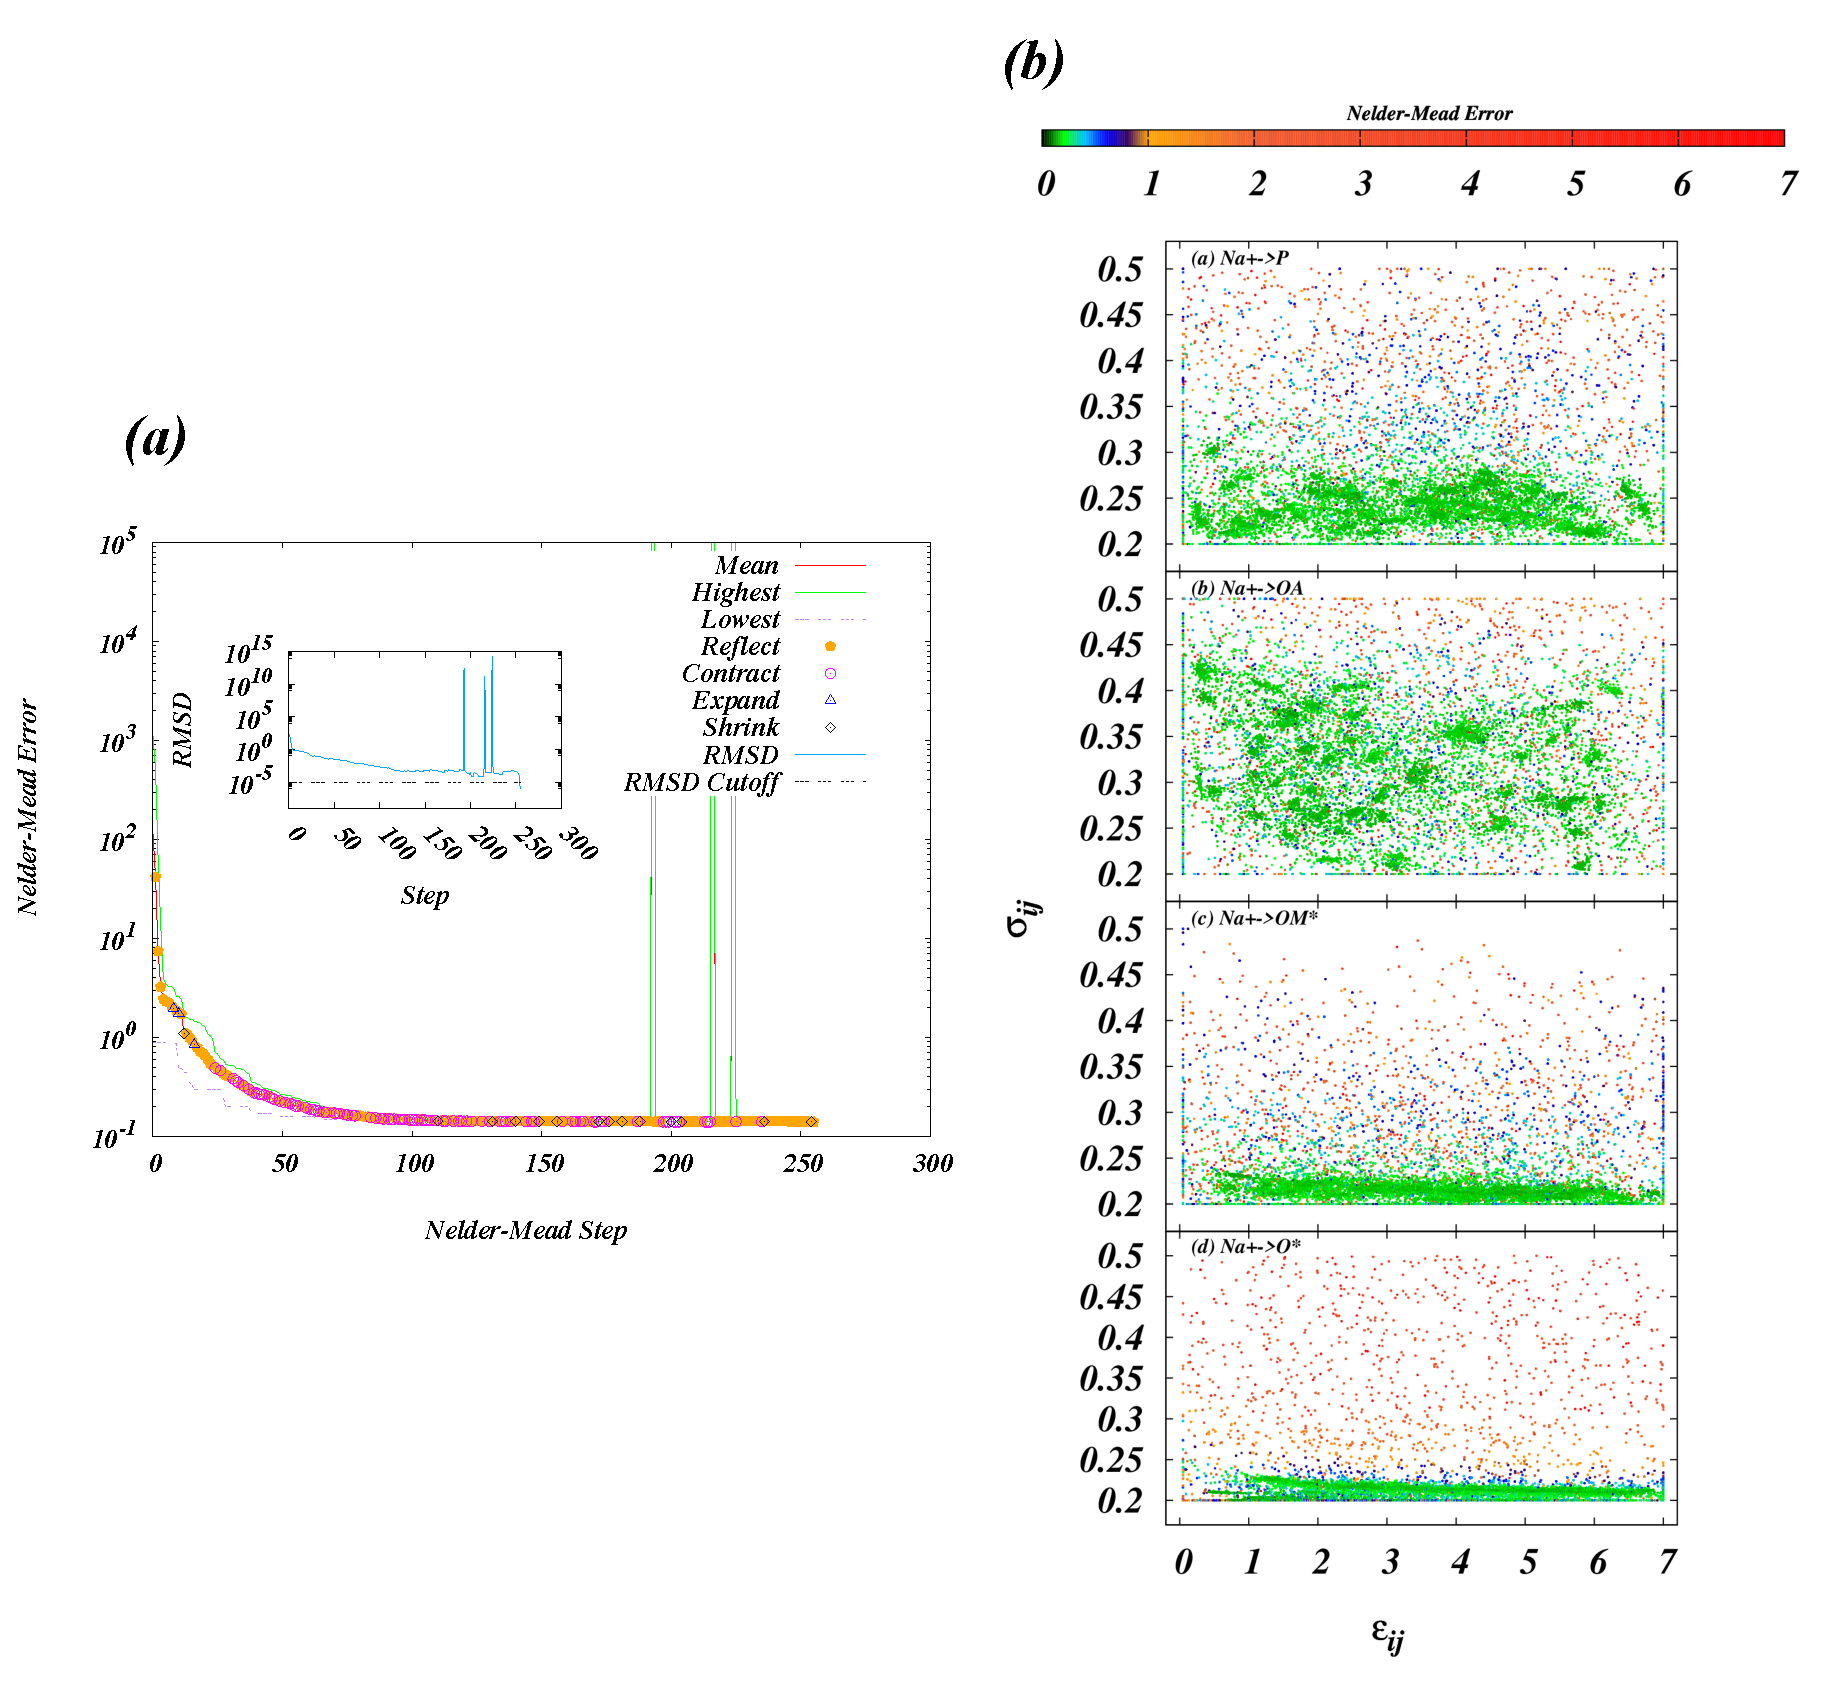
\includegraphics[width=0.7\textwidth]{figure_2.eps}
    \caption[Representative Nelder-Meade (NM) optimization run.]{(a) Representative Nelder-Meade (NM) optimization run. Each point
    represents a move that the NM simplex can make while navigating the parameter space 
    (See Fogarty \etal~for a full description of the
    Nelder-Meade algorithm and available moves~\cite{fogarty:2014:paropt}). The insert illustrates the 
    RMSD between the simplex vertices.
    The optimization is considered converged when the simplex collapses, which is defined by an RMSD~$\leq 10^{-10}$.
    (b) Map of all \sigmaij{} and \epsilonij{} tested for interactions of \na{} with non-carbon atom types 
    in the 200 optimizations performed to find our final optimized set of cross terms. A total of
291,870 combinations of parameters were tested, shown color-coded according to their NM error.}
    \label{figch2:nmerror}
\end{figure}
In this case, the NM-error is
defined as an
equally-weighted combination of the mean absolute error of the
substitution energy and the distances between each atom in the cluster and the \na{} ion. 
Each NM-move used is illustrated
as a point on the error curve 
(see Fogarty \etal{} for complete description of NM algorithm and
moves~\cite{fogarty:2014:paropt}).
The insert shows the root-mean squared distance (RMSD) between the simplex vertices at each step. 
As is typical with the NM method, error drops exponentially during the
initial steps, and slows down towards the end of the optimization
process. The termination condition for the optimization run is the
collapse of the NM-simplex (defined by the RMSD~$\leq 10^{-10}$).
Figure~\ref{figch2:nmerror}b shows all of the 291,870 \sigmaij{}-\epsilonij{} pairs tested 
between \na{} ions and the non-carbon atoms in the 200 independent optimization runs,
and provides a visual perspective of the sampled parameter space.
The parameter set that yielded the lowest error, as discussed in the results section, was
chosen to perform MD simulations of a POPC bilayer.
%The resulting parameter set was used to perform a simulation of a lipid
%bilayer in NaCl salt solution in order to further characterize
%the changes introduced.

\subsection{Bilayer Construction}

Simulation systems are constructed following the method outlined in chapter 1.
Based on a conservative estimate of one binding site per lipid,
at least 200 \na{} ions are required in bulk solvent to avoid depletion during
equilibration. To achieve this, I double the solvent block size used in our
previous work~\cite{kruczek:2017,kruczek:2019}, adding 60,000 waters to the
system on a three-dimensional grid and randomly replacing water molecules with
216 \na{} and 216 \cl{}. This corresponds to an initial concentration of 200~mM,
similar to our previous simulations, and yields a simulation box with initial
dimensions of $9.75 \times 9.75 \times 59.84$~nm$^3$. Following energy minimization as described in Chapter~1, 
the system is relaxed with a short NPT equilibration
at 290~K and annealed by heating to 350~K and cooling in 10~K steps to the
production temperature of 300~K (155~ps per step).

Following energy minimization and annealing, the box dimensions shrink to
$7.97 \times 7.97 \times 32.14$~nm$^3$. This final structure is used as the
starting point for production simulations.

\subsection{Molecular Dynamics}
Trajectories are simulated continuously for 0.7~$\mu$s to match the 
simulation length of Kruczek \etal{}\cite{kruczek:2017,kruczek:2019}.
Trajectory analysis is performed using a combination of GROMACS built-in
tools and in-house software developed on the GROMACS API.

\section{Results and Discussion}

\subsection{Optimized Cross-Terms}

The final optimized parameters are detailed in table~\ref{tabch2:paropt}
alongside the original parameters computed using LB rules. 
\begin{table}[H]
    \caption[Force-field cross terms]{Force-field cross terms. Original terms, as used in the system simulated with LB rules 
    were computed by applying Lorentz-Berthelot mixing rules to the LJ parameters of \na{} and each lipid component atom type. Optimized parameters are the 
    result of the NM-optimization using ParOpt~\cite{fogarty:2014:paropt,fogarty:2014:thesis}. All constraints
on the search space can be seen in figure~\ref{tabch2:constraints}}
    \label{tabch2:paropt}
    {\footnotesize
    \begin{tabularx}{\textwidth}{X|X|X|X|X|}
              &\tbxmulticol{2}{X|}{Original}&\tbxmulticol{2}{X|}{Optimized}\\\hline
              &\sigmaij{} (nm) &\epsilonij{} (kJ/mol) &\sigmaij{} (nm) &\epsilonij{} (kJ/mol)\\\hline
        NA-CH3&0.295&1.100&0.235&0.700\\
        NA-CH2&0.312&0.772&0.237&0.809\\
        NA-OA &0.256&1.120&0.211&3.035\\
        NA-P  &0.277&1.900&0.301&0.483\\
        NA-OM*&0.252&1.221&0.211&1.445\\
        NA-CO*&0.335&0.362&0.315&0.758\\
        NA-O* &0.251&1.221&0.216&2.440\\
              \end{tabularx}
          }
\end{table} 
One can Immediately note a general trend of an increase in the value of \epsilonij{} for the
non-carbon atom types. With the constraints on the carbon atoms, parameters have been nudged 
into gaining the binding energy by increasing the \epsilonij{} for the specifically electronegative atoms.
Values of \sigmaij{} have changed, but remained 
close to the original values in general, suggesting that the optimum 
distance to the minimum energy of the LJ potential is estimated well by LB rules. 
It can also be seen that no values of \sigmaij{} or \epsilonij{} violate the 
constraints described in table~\ref{tabch2:constraints}.
% \begin{table}
%    \caption{Nelder--Meade constraints. These values were used to constrain the parameter search space during the NM-optimization.}
%    \label{tabch2:constraints}
%    {\tiny
%    \begin{tabularx}{\textwidth}{X|X|X|X|X|X|X|X|X|X|}
%            &\tbxmulticol{2}{X|}{NA-CH3}&\tbxmulticol{2}{X|}{NA-CH2}&\tbxmulticol{2}{X|}{NA-CO*}&\tbxmulticol{2}{X|}{NA-OA,-OM*,-O*,-P}&Additional Constraints\\\hline
%        &Min&Max&Min&Max&Min&Max&Min&Max&N/A\\\hline
%    \sigmaij (nm)&0.2&0.5&0.2&0.5&0.2&0.5&0.2&0.5&$\sigma_{ij}^{\text{NA-OM*}}
%        \leq \sigma_{ij}^{\text{NA-P}}$ \\\hline
%    \epsilonij (kJ/mol) &0&0.79&0&0.81&0&0.83&0.05&7&N/A\\\hline
%    \end{tabularx}
%    }
%\end{table}
Substitution energies and corresponding conformational geometries are examined by running energy
minimization of the QM-optimized structures using the final parameter set. 
These are then analyzed using the GROMACS built-in energy and distance tools. 
The substitution energies and the conformations for
this parameter set are shown in figure~\ref{figch2:energies} 
and in figure~\ref{figch2:distances}, respectively. 
\begin{figure}[H]
    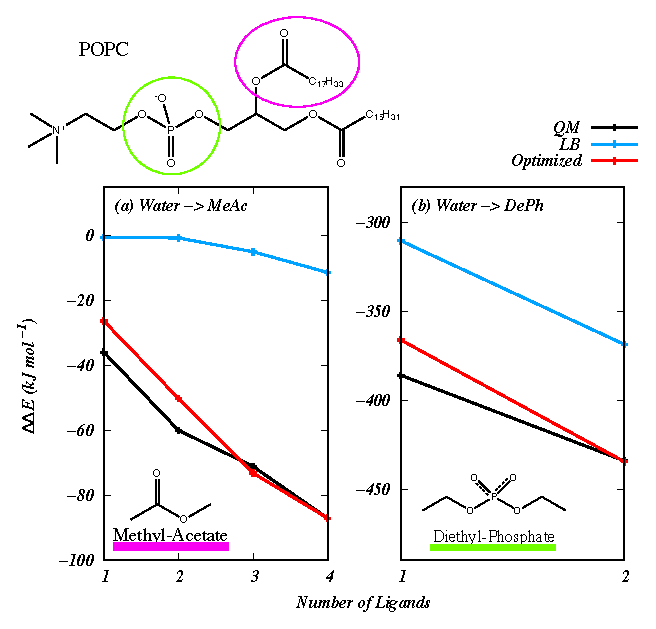
\includegraphics[width=0.7\textwidth]{figure_1.eps}
    \caption[Substitution energies for \na~clusters]{Substitution energies for \na~clusters computed as described
in equation~\ref{eq:substitution}. 
The energies of systems computed using the standard 
mixing rules are shown in black, the energies from benchmarked DFT are in red, 
and in blue are the optimized results. 
There is a significant
error with the standard LB mixing rules, which is substantially improved with the new optimized cross terms. 
The insert shows an diagram of POPC, and
the small molecules Methyl-Acetate (MeAc) and Diethyl-Phosphate (DePh) 
that were used to represent the major \na~interaction sites on the POPC molecule.}
    \label{figch2:energies}
\end{figure}
\begin{sidewaysfigure}[H]
    \centering
    \caption[Distances from \na{} to each component atom in sample clusters]{Distances from \na{} to each component 
    atom in sample clusters. The geometry of our sample clusters is found by computing the distance from
    the ion to each other atom in the system, shown per atom type.
    These distances are used in combination with the substitution energies in figure 2 to compute the
error for the NM optimization.}
    \label{figch2:distances}
    %\includegraphics[width=0.8\textheight]{distances_combined_final.eps}
    \includegraphics[width=0.8\textheight]{figure_s1.eps}
\end{sidewaysfigure}
It can be noted that for MeAc there is substantially improved substitution
energies relative to those obtained from using LB mixing rules, 
which started with an discrepancy of around 30--80~kJ/mol. The optimization has also
improved the relative substitution between the clusters of various sizes. 
The substitution energies for DePh have also improved by a similar magnitude. 
The conformational geometries are largely unchanged, 
with a general trend of the binding distance to OM\* shrinking on the order of 0.25~\AA~in DePh. 
This shrinkage is common when optimizing both energies and conformations
with the relatively small number of free parameters corresponding to
the LJ cross terms~\cite{wineman:2019}.

Notably, the substitution energies for both molecule types improve more in the
larger cluster sizes. Larger clusters are more relevant to the dense
environment in the lipid headgroup region of the bilayer, 
as few, if any, ions bind to a single lipid at a time~\cite{kruczek:2017}. 
Furthermore, the substitution energy profile for MeAc has become much closer to that of the QM profile. 
Thus, these new parameters substantially improve the energetic balance
between the lipid-ion, lipid-water and ion-water interactions.

The conformational geometries were mostly unchanged with the new
parameter set, as even the original parameters do a good job in reproducing the QM-configurations. 
The least precise cluster appears to be for 4 MeAc, 
where the original LB parameters poorly represent the symmetries exhibited in the QM data. 
Even with the improvement from our new parameters, 
there may be missing behavior from explicit polarization effects that
cannot be captured properly by a non-polarizable model~\cite{varma:2010}.

\subsection{Validation of Parameters}

In order to characterize our new parameter set in a bilayer, 
I generated a 700~ns simulation of a bilayer of POPC lipids in NaCl salt solution, 
and the results are compared against a similar system simulated using
LB rules in previous work~\cite{kruczek:2017,kruczek:2019}. 
These older trajectories for systems both with salt and without will be referred to, 
respectively, as  LB and `without salt.'  
New simulations are performed with optimized cross terms, 
hence forth will be referred to as the `optimized' system, 
long enough to equilibrate the number of bound ions (see figure~\ref{figch2:ioncoodcount}). 
This ion binding is further characterized in a subsequent section.

\subsubsection{Bilayer Structure}

Bilayer structural parameters can be seen in table~\ref{tabch2:struc}.
\begin{table}[H]
    \caption[Bilayer structural parameters]{Bilayer structural parameters. \dhh{} is the peak-to-peak distance from the electron density of the
        lipid bilayer, and is a measure of bilayer thickness. Bilayer thickness \db~and chain thickness \dc{} are computed from
        number densities of the solvent and the lipid chains, respectively. $V_H$, and $V_C$ are the volumes of the headgroup and lipid chains computed
        using the method from Petrache \etal{}\cite{petrache:1997}. $V_L$ is the sum of $V_H$ and $V_C$. 
        Rows 7-11 contain kinetic parameters for ion binding to membrane. These parameters come from fitting 
        the equation $ N_b(t)= \frac{K_{a}}{K_{a}+K_{d}} 
            N\left(1-\exp\left[-\left(K_{a}+K_{d}\right)\left(t-t_0\right)\right]\right)$ to the data for the number of ions
            bound to the lipid bilayer across the simulation time. 
            $A$ is the asymptotic number of ions bound to the lipid bilayer, and can be used as the expected number of ions
        that will bind to the system at equilibrium. $\tau$ is the characteristic timescale of the fitted function. $n_0$ is the number of ions bound at the beginning
        of the production run of the simulation. $K_D$ and $K_A$ are the computed binding association and dissociation constants, and $K_A/K_D$ is the binding
    rate constant.}
    \label{tabch2:struc}
    {\footnotesize
    \begin{tabularx}{\textwidth}{X|X|X|X}
         &Without salt      &LB                 &Optimized\\\hline
        $D_{HH}$~(\AA)&37.44 $\pm$ 1.07  &40.18 $\pm$ 1.04   &37.64 $\pm$ 0.88 \\
        $D_B$~(\AA)   &36.54 $\pm$ 0.47  &40.90 $\pm$ 0.31   &39.36 $\pm$ 0.43\\
        $2D_C$~(\AA)  &27.07 $\pm$ 0.34  &30.33 $\pm$ 0.29   &28.97 $\pm$ 0.34     \\
        $V_H$~(\AA$^3$) &310.68 $\pm$ 1.14 &316.13 $\pm$ 0.83  &314.81 $\pm$ 0.75          \\
        $V_C$~(\AA$^3$) &904.89 $\pm$ 1.28 &891.79 $\pm$ 1.65  &896.50 $\pm$ 1.19         \\
        $V_L$~(\AA$^3$) &1215.57 $\pm$ 1.00&1207.92 $\pm$ 1.57 &1211.32 $\pm$ 1.21    \\
        $K_{A}$ (ns$^{-1}$)        &N/A & $7.12\times10^{-3}\pm8.18\times10^{-5}$     &$2.65\times10^{-3}\pm1.74\times10^{-5}$ \\
        $K_{D}$ (ns$^{-1}$)        &N/A & $3.20\times10^{-3}\pm4.75\times10^{-5}$     &$3.58\times10^{-3}\pm2.83\times10^{-5}$ \\
        $A$                        &N/A & $74.51$                        &$91.88$ \\
        $\tau$      (ns)           &N/A & $96.73$                      &$160.54$ \\
        $K_{A}/K_{D}$              &N/A & $2.225$                           &$0.74$ \\
              \end{tabularx}
          }
\end{table}
The phospholipid component volumes $V_H$ and $V_C$ (lines 1 and 2) are
computed following the procedure outlined by Petrache \etal~\cite{petrache:1997}, and described at length in chapter 1 of this dissertation. 
The total lipid volume $V_L$ (line 3 in table~\ref{tabch2:struc}) 
is taken to be the sum of these two values. 
These remain relatively similar in all three systems, 
as this value is intrinsic to the lipid molecule 
and should not change with the inclusion of ions.

Structural data are obtained for lipid bilayers via small angle X-ray and neutron scattering
experiments as a one-dimensional form-factor. Data are then
fitted to a continuous function to retrieve number and electron
densities for the various lipid components~\cite{nagle:2000,fogarty:2015}. 
Our simulations allow us direct access to the electron densities and number densities. 
The entries in table~\ref{tabch2:struc} are determined from these densities.

Figure~\ref{figch2:eldens} shows the electron densities and corresponding bilayer form-factors.
\begin{figure}[H]
    \caption[Electron densities of the simulated bilayers]{Electron densities of the simulated bilayers (a), and corresponding bilayer form-factors (b).
        Electron densities as obtained using the GROMACS density tool,
    centered at the minimum to define the bilayer center, and with the electron density of solvent subtracted.
    The simulated with optimized parameters appears to lack the large peak seen in the system simulated
    with LB rules, and appears more similar to the
bilayer structure of a bilayer simulated without salt. 
This is further reflected in the bilayer form-factor, 
computed by taking the cosine-transform of electron density. Experimental
SAXS results are for a POPC bilayer in pure solvent~\cite{fogarty:2015}. We see the first lobe
of the optimized system moves closer to the experimental results and the form-factor of a system without salt. This lines up with experimental results, that have shown small, if any, change
in the bilayer SAXS form-factor~\cite{pabst:2007,petrache:2006:swelling,uhrikova:2008}.}
    \label{figch2:eldens}
    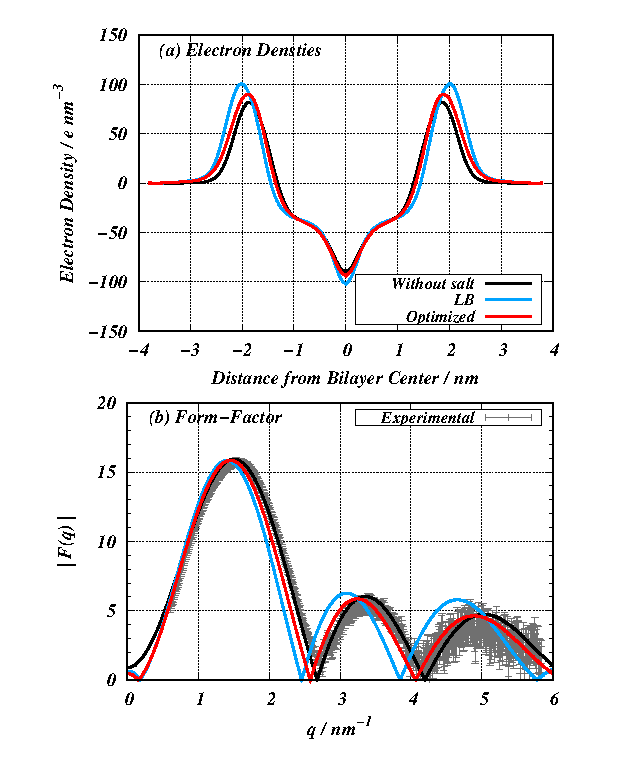
\includegraphics[width=0.7\textwidth]{figure_4.eps}
\end{figure}
Form-factors are computed by taking the cosine-transform of the symmetrized electron densities.   
It can be noted that the simulations carried out using LB rules produced a
thicker bilayer and had different details at the peak region of the density. 
The new parameter set results in similar electron density to that of the system without salt.
This is similar to the results reported by Petrache
\etal{} and Pabst \etal{}, where for systems with less than 1~M NaCl, 
the differences in the electron densities were not
discernible~\cite{petrache:2006:swelling,pabst:2007}. 
These electron densities are used directly to measure the value of \dhh{}, 
defined as the peak-to-peak distance (see table~\ref{tabch2:struc} line 4). 
The new parameter set corresponds to a smaller \dhh{}, similar to the system without salt.

In addition to \dhh{}, different measures are used to assess the bilayer thickness 
that relies on the probability densities of different components of the system.
It can be shown that \db{}(see table~\ref{tabch2:struc} line 5) computed by integrating one minus
the probability density of solvent and ions is equivalent to the computation of the 
Luzzati thickness of the total bilayer~\cite{fogarty:2015,chiu:2009}.
Probability of finding a particular component in a slice of the box is defined as,
\begin{equation}
    \label{eq:probability}
    P_{i}(z) = \frac{\rho_i(z)}{\sum^n_{j}\rho_{j}(z)}\text{,}
\end{equation}
where $\rho_{i}(z)$ are the number densities for the 
component particles ($i$) of the system as a function of the 
z-position of each slice of the box, and the summation
ranges over all components in the particular slice.
Thus, 
\begin{equation}
\text{\db}=\int_{\text{Box length}}\big(1-P_{\text{water}+\text{ions}}(z)\big)\;dz\text{.}
\end{equation}
In table~\ref{tabch2:struc} line 2, the \db{} is larger for the systems
with ions, but the value obtained using our new parameter set is closer to that of
the bilayer simulated without salt.

A similar definition of probability density is used for \dc{}, 
computed from the probability distribution of the lipid chains. 
This component is defined by the hydrocarbon chains starting after the ester-linkage
on both the Sn1 and Sn2 terminal of the lipid backbone. 
This value (line 6 in table~\ref{tabch2:struc}) is increased in the system simulated
with LB rules over the system without salt, 
as is reported in our previous work. 
However, the new parameter set yields a value similar to the system without salt, 
which is consistent with the smaller overall thickness of the bilayer 
simulated with optimized cross terms.

The differences in bilayer thickness are closely related to the
packing of the lipid chains in the hydrophobic core of the bilayer. 
When the chains become more disordered, 
the bilayer thickness typically drops~\cite{nagle:2000}. 
This ordering is described by the acyl-chain C-D order parameter, 
plotted per each carbon in the lipid chain in figure~\ref{figch2:op}. 
\begin{figure}[H]
    \caption[Lipid chain deuterium order parameters.]{ Lipid chain deuterium order parameters. $S_{CD}$s are computed for each carbon
        for the chains Sn1 (a) and Sn2 (b), starting at the second carbon in the chain. We see that the optimized system is still showing significant ordering in the lipid
    chains as a result of ion binding; however, the ordering is less pronounced than in the system simulated with LB rules, 
    and is closer to that of the simulation without salt. This
result corresponds with the smaller bilayer thickness in the optimized system.
}
    \label{figch2:op}
    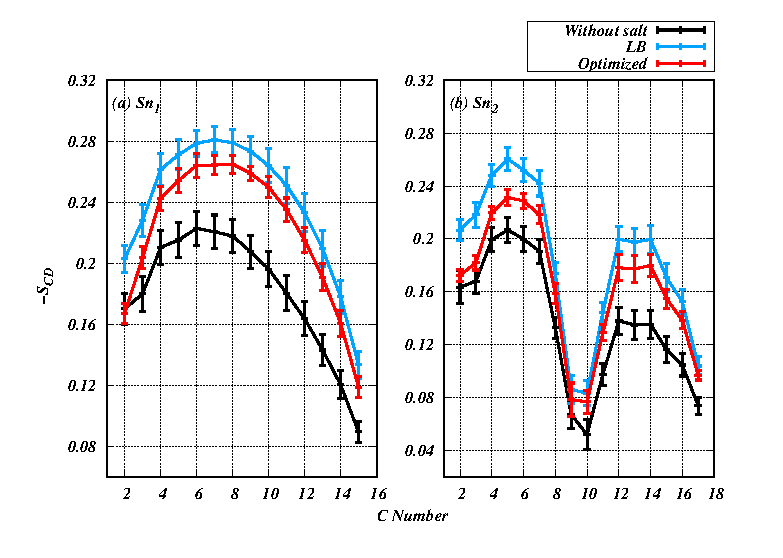
\includegraphics[width=0.7\textwidth]{figure_s2.eps}
\end{figure}
As reported in our previous simulations, 
the addition of salt has an ordering effect on the lipid chains. 
This effect is also seen in our new parameter set; however, the ordering is less pronounced, 
which is consistent with the notion that the bilayer structure is not significantly altered 
at physiological salt concentration~\cite{pabst:2007,petrache:2006:swelling}.

While this result indicates a structure more consistent with experimental results, 
the detailed structure of a lipid bilayer is a result of the
delicate balance between ion-lipid, lipid-water, and ion-water interactions.
In order to fully understand how our new parameter set has altered the
overall bilayer structure, we next characterize the specific interactions
between these moieties.

\subsection{Membrane-Salt Interactions}

Both ions and solvent compete for the binding sites on the lipid headgroup. 
As seen in figure~\ref{figch2:energies}, the new cross terms
produce a relatively stronger interaction between \na{} and lipid
headgroup components compared to that of the LB rules. 
Thus, there is potentially a reduction in the available binding sites for the solvent. 
To examine how the new cross terms have altered ion interactions with lipids in the bilayer, 
I first characterize the dynamics of ion binding to the lipid bilayer.

I define ion binding to the lipid bilayer when half or fewer
of its first shell coordinators are not waters. 
In order to compute the equilibrium binding constant, 
one must determine the equilibrium number of bound ions to the lipid surface. 
Figure~\ref{figch2:ioncoodcount} shows the number of bound ions as a
function of time over the entire duration of the simulation. 
\begin{figure}[H]
    \includegraphics[width=0.7\textwidth]{figure_3.eps}
    \caption[Number of ions bound to the lipid bilayer]{Number of ions bound to the lipid bilayer as a function of simulation time. 
The exponential fits to this data are also shown. These fits are used to compute the asymptotic
number of ions bound as well as binding rate constants.
`Total' refers to the total number of ions in each simulation box.
A membrane bound ion is defined as having half or fewer of its first coordination shell
occupied by water molecules. }
    \label{figch2:ioncoodcount}
\end{figure}
It can be noted that even after 700~ns of simulation time, the number of bound ions
are not fully equilibrated. 
Thus, first-order reaction kinetics are used to
estimate the asymptotic number of bound ions.  
The first-order reaction kinetics are modeled as a differential equation:
\begin{equation}
    \frac{dN_b}{dt}=K_a \left(N-N_b\right)- K_d N_b,
\end{equation}
where $N_b$ are the number of bound ions, and $K_a,K_d$ are the association and dissociation
time constants, respectively.
The solution of this differential equation is:
\begin{equation}
    N_b(t)= \frac{K_{a}}{K_{a}+K_{d}} N
    \left(1-\exp\left[-\left(K_{a}+K_{d}\right)\left(t-t_0\right)\right]\right).
    \label{eq:ioncoodnumfit}
\end{equation}
This solution is fit to the data in figure~\ref{figch2:ioncoodcount}, 
and the resulting fit is also plotted. 
The fitting parameters are listed in table~\ref{tabch2:struc}.
The first-order reaction kinetic model fits reasonably well to the 
data from both the systems, except in the beginning of
the simulation where the effect of the annealing process is more pronounced; 
however, only the asymptotic
behavior of the fit is interesting as this is representative of the equilibrium state of the system. 
The asymptotic number of bound ions as $t\to\infty$, $A=\frac{K_{a}}{K_{a}+K_{d}} N$ 
(table~\ref{tabch2:struc} row 9), is larger in the system simulated with optimized terms.
The timescale of ion binding $\tau=\frac{1}{\left(K_{a}+K_{d}\right)}$ is also reported 
for both systems (table~\ref{tabch2:struc} row 10). 
The timescale of binding in the system using optimized cross terms is longer, 
and suggests that this system would need more time to equilibrate than the system simulated with LB rules.
Finally, the value of $\frac{K_a}{K_d}$ is reported
(table~\ref{tabch2:struc} row 11), which
one can observe is much smaller with the new parameter set than compared to that
of the system simulated with LB rules.

To examine how specific interactions between ions and lipids are modified by the new parameters, 
I tracked the binding partners of ions across the box over the last 150~ns of simulation time. 
Moieties are considered to be bound to an ion if they are within a distance of 3.3 \AA{} from the \na{} ion. 
Several electronegative groups in the simulation can potentially bind to the \na{} ion. 
The number of these potential binding partners within the first shell of each \na{} ion
across the simulation box is computed. 
Ions are then sorted according to their box z-positions, and then the data are averaged over the last 150~ns. 
This is plotted in figure~\ref{figch2:cood}. 
\begin{figure}[H]
    \caption[\na{} inner shell coordination partners]{Chemistry of \na{} inner shell coordination as a function of distance from bilayer
center. Compared to the system simulated with LB rules (a), the system simulated with optimized cross terms (b)
        yields a lower \na{} total coordination number within the headgroup region of the bilayer. 
        This drop in coordination appears to be due to a greater dehydration of the ions in this system.}
    \label{figch2:cood}
    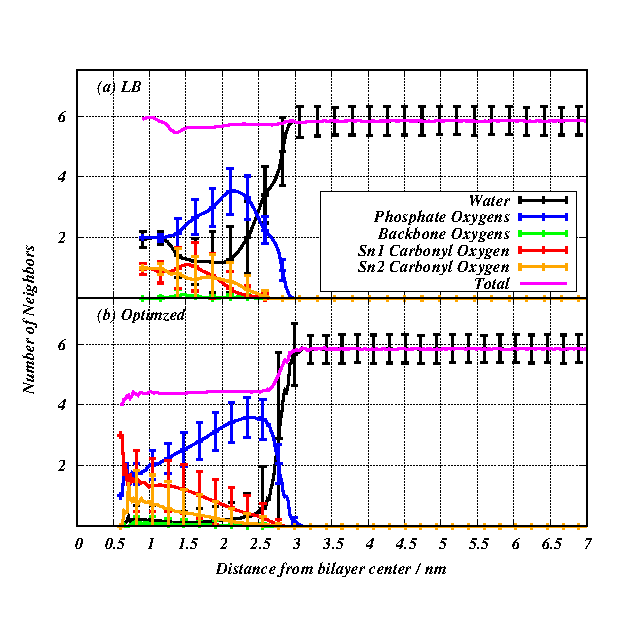
\includegraphics[width=0.7\textwidth]{figure_5.eps}
\end{figure}
It is noted that the total number of solvating oxygens of ions within the bilayer headgroup
region with the optimized parameter set has dropped by $\sim 1$ when
compared to ions in similar locations in the system simulated using LB rules. 
This is not surprising, given the dependence of ion coordination
preferences on the local environment~\cite{varma:2008:JACS}. 
The binding to other lipid oxygens has not been altered much by the new parameter set; 
however, we do note that water within the headgroup region does not appear to be strongly associated with ions. 

\subsection{Water Structure and Dynamics}

To further characterize the dehydration of ions in the new simulated system, 
we look to the lipid- and ion-water interactions.
Figure~\ref{figch2:waterdens} shows the number density of water as a
function of distance from the bilayer center for each of our simulated
systems, with the \dc{} and \db{} illustrated as dotted lines.  
\begin{figure}[H]
    \caption[Water density at the bilayer interface]{ Water density at the bilayer interface. We illustrate the regions $B_{-1}$, $B_+$, $B_{-2}$ and $Bulk$ for each system with dotted lines.
    We see that the optimized cross terms yield a greater density 
    of solvent in the $B_{+}$ and $B_{-1}$ regions over the system simulated with LB rules. 
We also see the density in these regions of the system optimized
with optimized cross terms is more similar to that of the system without salt.}
    \label{figch2:waterdens}
    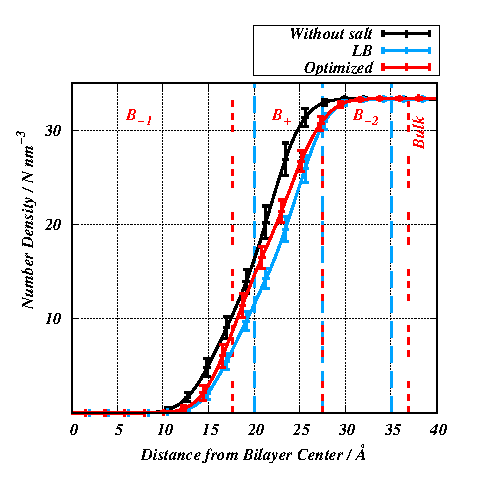
\includegraphics[width=0.7\textwidth]{figure_6.eps}
\end{figure}
It can be seen that our new parameter set produces a bilayer
interface that has more solvent inside the headgroup region, 
between $10-25$~\AA~from the bilayer center. 
This density is more similar to that of the system simulated without salt. 
This suggests that the dehydration of ions in the system simulated with optimized parameters
does not correspond to a dehydration of the lipid bilayer.

Next, the orientational structure of the water is calculated following the procedure outlined in chapter 1.
Figure~\ref{figch2:waterorder} examines the water order parameter across the simulation box. 
\begin{figure}[H]
    \caption[Water orientational order parameters]{ Water orientational order parameters $P_1$ (a) and $P_2$ (b), 
and the product of the water number density and $P_2$ (c). We see in $P_1$ and $P_2$ less
    ordering in the waters in the optimized system, suggesting that waters may be less strongly interacting with ions or lipid components. We denote the four regions of the lipid bilayer based on the shape of the $P_2$ data as dotted lines
    in (b)~\cite{saunders:2019}. We have not included these regions
 for the system without salt, as the $P_2$ data does not include the same details as the systems with salt. The integral of (c) is related to the
 quadrupolar splitting constant $\Delta \nu$ found in deuterium NMR experiments. This also gives a closer look at how solvent is ordered in the headgroup while
 accounting for the amount of solvent in the region. We see that optimized cross terms result in a significant drop in the area under the curve, which is much closer
 to the shape of the data from the system without salt. 
 The regions $B_{-2}$ and $Bulk$ are not within the bilayer
headgroup, and are expected to be less affected by the new parameter set.}
    \label{figch2:waterorder}
    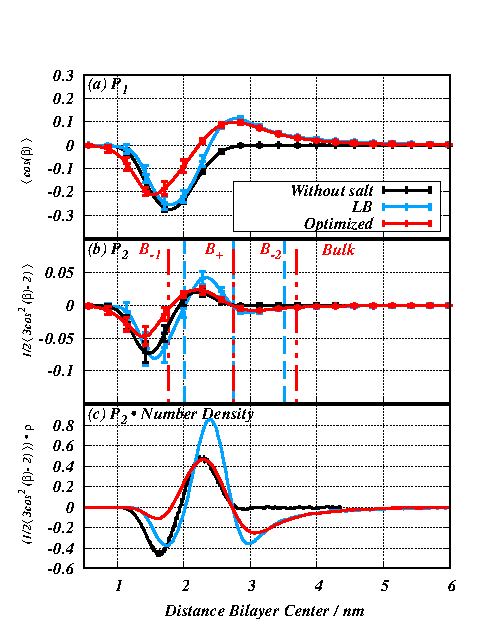
\includegraphics[width=0.7\textwidth]{figure_7.eps}
\end{figure}
A similar pattern of ordering across the box in all systems can be observed; 
however, we see an overall reduction in ordering with our new parameter set when
compared to both the LB and the no-salt system. 
We also see the inner minimum of the order parameter moved further into the bilayer
when compared to LB, 
which is consistent with the larger quantity of water 
in this region that we observe in the water densities.

Following the protocol established in our previous work~\cite{saunders:2019}, 
three regions within the bilayer interface are identified, $B_{-1}, B_{+}, B_{-2}$. 
The $B_{-1}$ region is defined as the region of negative ordering starting at the bilayer center, and ending 
    when the order parameter values cross zero at the start of the $B_{+}$ 
    region. The $B_{+}$ region starts at the end of the $B_{-1}$ region, and 
    is the area of positive ordering, ending where the order parameter crosses
    zero again. The $B_{-2}$ region starts at the end of the $B_{+}$, and extends out to where the 
    second order parameter goes to zero. This was found by fitting an exponential function to this region 
    and taking the \replaced{scale parameter}{timescale} from that fit as the boundary with bulk solvent.
Water is significantly less perturbed by the bilayer with our new parameter set.  
We have also computed $P_2\cdot\rho_{\text{Water}}$, shown in shown in figure~\ref{figch2:waterorder}(c). 
This value relates the amount of water in each region of the box and 
the overall ordering in the region. 
We still see significantly less ordering with the new parameter set, 
and even with the larger number of waters in the bilayer headgroup. 
The integral of this curve is related to the quadrupole splitting $\Delta \nu$ observed in
in deuterium NMR experiments~\cite{aaman:2003,kruczek:2017}.

This suggests that while there is more solvent in the interface, it is perhaps not
associated with either \na{} or lipids, and may remain less structured than
in the system simulated with LB rules.  
This can be further ascertained by the lateral diffusion coefficients of waters 
in each of the regions defined by $P_2$. 
We compute the mean square displacement (MSD) for water oxygens
in each region by first tracking which waters remain in the region. 
Any waters that leave the region are removed from the MSD calculation. 
We chose a duration of 100~ps to track the MSD in order
to have a sufficiently long time for the MSD to become linear, 
while still maintaining a statistically significant number of waters in the slice. 
A line is fit to the middle 80\% of the MSD, and the fitted
slope is used to calculate the diffusion coefficient following
Einstiein's relation for 2D diffusion
\begin{equation}
\lim_{t \to \infty}\frac{\big\langle (r(t) - r(0))^2 \big\rangle}{(t-t_0)} = 4D. 
\end{equation}
These values can be seen in table~\ref{tabch2:diff}. 
\begin{table}[H]
    \caption[Diffusion coefficients of water in different regions]{Diffusion coefficients of water in different regions of the lipid bilayer, 
defined by the shape of the second orientational order parameter of water molecules in the box. 
These regions are defined by the shape of the distribution of the second 
    orientational order parameter across the simulation box. $B_{-1}$ is the region 
    of negative ordering starting at the bilayer center, and ending 
    when the order parameter values cross zero. 
    $B_{+}$ starts at the end of the $B_{-1}$, and is the region of positive ordering ending where the order parameter 
    becomes negative. This starts the $B_{-2}$ of negative ordering, extending out to where the 
second order parameter goes to zero, where we have $Bulk$ solvent.
We see that the optimized parameters result in slightly 
    increased diffusion in the solvent, which correlates with the reduced
    ordering of the water dipoles and quadrupoles in the
system.}
    \label{tabch2:diff}
    {\footnotesize
    \begin{tabularx}{\textwidth}{X|X|X|}
              &LB ($\times 10^{-10} m^2/s$)&Optimized ($\times 10^{-10} m^2/s$)\\\hline
        $B_{-1}$ &1.11 $\pm$ 1.10& 1.88 $\pm$ 2.41   \\
        $B_+$    &4.23 $\pm$ 1.14& 6.11 $\pm$ 2.83  \\
        $B_{-2}$ &18.11 $\pm$ 4.23&21.29 $\pm$ 4.12 \\
        $Bulk$   &27.32 $\pm$ 1.15 &27.25 $\pm$ 1.36 \\
              \end{tabularx}
          }
\end{table}
We note that the water in the headgroup region, corresponding to $B_{-1}$ and $B_+$, 
diffuses slightly faster with the new parameter set, 
indicating more mobile water in these regions. 
However, the computed diffusion coefficients are within the error bars that of the system simulated with LB rules. 
Diffusion in the $B_{-2}$ and $Bulk$ regions are similar in both systems, 
as these are mostly outside of the bilayer and should not be affected by the new parameter set.


\subsection{Bilayer Electrostatics}

We further characterize the electrostatic properties of our bilayer
systems by computing the electrostatic potential across the simulation box. 
We do this following the protocol used in Saunders \etal{}
~\cite{saunders:2019}. First, the charge density of the
system components is obtained. This is then integrated twice, with both
constants of integration set to be zero to enforce a zero value for the
electric field in bulk solvent and a zero electrostatic potential at
the box edge. This is accomplished by taking the average value of the
electric field in the \emph{bulk} region of the box defined earlier,
and subtracting this value from all points. Due to the larger system
size in the optimized system, the average value of a much
larger region than in LB is needed in order to apply boundary conditions. This is then
integrated again to get the electrostatic potential. This result
can be seen in figure~\ref{figch2:potential}. 
\begin{figure}[H]
    \caption[Bilayer electrostatic potential]{ Electrostatic potential as a function of distance from bilayer center. The optimized
cross terms yield a small change in the location of the peak of the potential in the
bilayer simulated with optimized cross terms, as well as the loss of the valley behind the peak.
}
    \label{figch2:potential}
    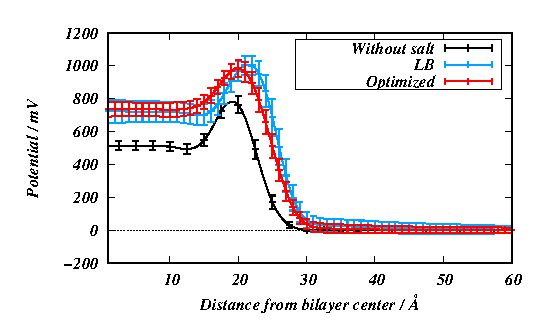
\includegraphics[width=0.7\textwidth]{figure_s3.eps}
\end{figure}
The shape of the potential
is largely unaltered within fluctuations. Systems simulated with the
optimized parameters and with LB rules both have a similar bilayer dipole potential, 
which remains elevated over
the system without salt, by $\sim$ 220~mV.  We report 
that the optimized system has a slightly
elevated bilayer dipole potential compared to the system simulated with
LB rules, increased by $\sim$ 12~mV.
This may be a direct result of the larger number of
ions bound to the bilayer in this system.  It can also be noted that the system simulated with optimized cross terms
has different details
throughout the electrostatic potential compared to the system simulated with LB rules; However, in the
system without salt these are within fluctuations and cannot be used to draw conclusions.

Poisson-Boltzmann (PB) theory is a mean field approximation for
solvated ions near an interface. Experimentally PB theory is used to
assess the surface potential of the lipid bilayers. We also examine
the behavior of the ions in bulk solvent under the framework of PB
theory. Following the procedure used in our previous
work~\cite{saunders:2019}, we fit the number density of \cl{} ions in
the solvent-occupied region of the box to a Poisson-Boltzmann
distribution, using the inverse Debye length $K$ and the density of
\cl{} at the center of the solvent occupied region of the box $\rho_0$
as fit parameters. 
The density is modeled as:
\begin{equation}
    \label{eq:gcdens}
    \rho (z)= \rho _{0} \exp{(- \bar{z} e \beta \psi (z))},
\end{equation}
where $\rho_0$ is the number density of the ion at the center of the
solvent-occupied region of the box, $\bar{z}=1$ is the valency of the
ion in the system, $\beta=\frac{1}{k_b T}$, $e$ is the charge on an
electron, and $\psi(z)$ is the electrostatic potential. We then assume
the form of $\psi(z)$ to be the sum of two Debye-Huckel
potentials~\cite{israelachvili:2011:intermol} reflected across the
center of the solvent-occupied region of the box:
\begin{equation}
    \begin{split}
    \psi_1(z)&=\psi_s \exp(-K(z+\frac{D}{2})) \\
    \psi_2(z)&=\psi_s \exp(K(z+\frac{D}{2})) \\
    \psi(z)&=\psi_1 + \psi_2\text{,}
    \label{eq:gcpot}
\end{split}
\end{equation}
where $D$ is the distance from the hydration boundary of one bilayer leaflet
to the next across the solvent, $K$ is the inverse Debye length, and $\psi_s$ is the surface potential:
\begin{equation}
    \psi_s = \frac{\varsigma}{\varepsilon_0\varepsilon K}\text{.}
\label{eq:gcspot}
\end{equation}
%, given by
%\begin{equation}
%K=\sqrt{\sum_i{\rho_{0,i}\bar{z^2_i}\frac{e^2}{\epsilon_0 \epsilon k_bT}}}
%\label{eq:gcK}
%\end{equation}
The LB system yielded a value of $D=13.167$ nm and the system
simulated with optimized parameters, containing twice as many 
solvent molecules,
gave a value of $D=27.01$ nm.
The surface charge density $\varsigma$ is taken from the charge density inside
of the hydration boundary of the lipid bilayer. Since only ions
contribute a net charge to our system, this is computed using only the
charge density of ions in the system. 
This value was computed to be $\varsigma=0.13$ \emph{e} nm$^{-2}$ for the system simulated with LB rules, and 
$\varsigma=0.11$ \emph{e} nm$^{-2}$ for the system simulated with the new parameters.
Our fitting procedure yielded 
number densities $\rho _{0}=0.043\text{nm}^{-3}$ for the system simulated with LB rules, 
and $\rho _{0}=0.079\text{nm}^{-3}$ for the system simulated with optimized parameters.
The fitted inverse screening lengths were found to be $K=0.91 \pm 0.014$ nm$^{-1}$ for the LB rules simulation 
and $0.94 \pm 0.018$ nm$^{-1}$ for the system simulated with optimized parameters.
The resulting fit and predicted
density of \na ions and electrostatic potential can be seen in
figure~\ref{figch2:gouy}. 
\begin{figure}
    \caption[Poisson-Boltzmann theory predictions and simulation results.]{
        Poisson-Boltzmann theory predictions and simulation results.\ (a) shows a snapshot of the 
system simulated with optimized cross terms, translated
to center the solvent occupied region. Water has been hidden
for clarity.\ (b) and (d)
    show the number density of ions in the solvent occupied region of the box. 
    (c) and (e) show the corresponding electrostatic potential in solvent.
    Theoretical predictions are illustrated as solid lines, with corresponding 
    simulation results as points with error bars. Red vertical lines denote the \emph{hydration boundary} of the lipid bilayer. 
    \cl{} density data is used for fitting in both systems. 
}
    \label{figch2:gouy}
    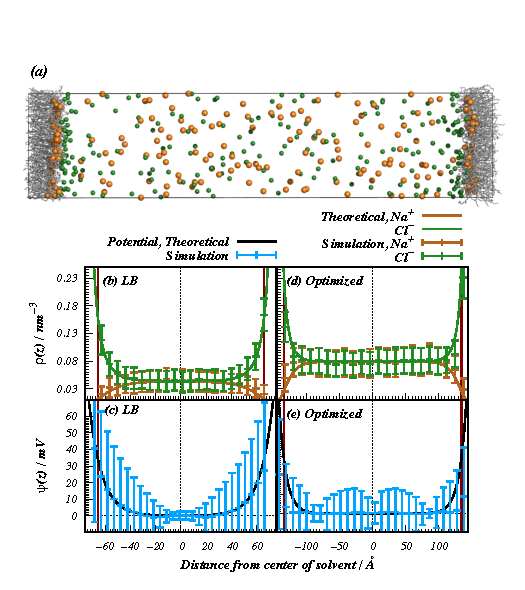
\includegraphics[width=0.7\textwidth]{figure_s4.eps}
\end{figure}
The results from our simulation are
represented by points with error bars, while PB theory results are
shown in solid lines.  This shows excellent agreement in the \na{} density
profile away from the bilayer surface, and reasonable agreement in the
electrostatic potential. From this one can see that the optimized and LB
systems both exhibit similar ionic distributions with models used to
describe electrophoretic mobility
experiments~\cite{israelachvili:2011:intermol}.

\section{Conclusions}

Mixing rules are often relied upon to compute non-bonded cross terms 
for interacting molecules in molecular simulations. 
However, when mixing force-fields that have been developed independently of each other, 
inaccuracies may develop. 
Here I demonstrate one such case and propose a rigorous solution. 
MD simulations conducted using predefined mixing rules for 
non-polarizable force fields developed separately for ions and lipids 
have always produced very pronounced salt-induced structural changes in lipid bilayers. 
Contrary to this, most experimental observations point to a 
moderate or even an insignificant change in bilayer structure at physiological salt concentrations. 
This discrepancy is resolved by explicitly parameterizing ion-lipid cross terms
using our procedure {\em ``Many Body Non Bonded fix''} (MB-NB-fix). 
It is based on the NB-fix method employed in previous works
~\cite{baker:2010:accurate,yoo:2012:improved,fyta:2012:ionic,mamatkulov:2013:force,venable:2013,savelyev:2014:balancing,li:2015:representation,savelyev:2015:competition,jing:2017:study}
and utilizes ParOpt software developed in our lab~\cite{fogarty:2014:paropt}\cite{fogarty:2014:thesis}.
It is noted that after applying the optimized parameters for \na-lipid interactions, the 
bilayer structure conforms more to experimental
observations. It is also noted that all other properties such as solvent structure,
electrostatic potential, and dynamic properties are approximately
similar to that obtained with those obtained with LB parameters. 
We note that we have not applied this method to optimize \cl{} interactions terms, which
may still further affect the bilayer structure. This will be the subject of future work.

The MB-NB-fix method proposed here is a 
general method which can be used to derive mixing
terms for simulations with independently developed force fields. 
This method will be used in future work to improve other sets of mixed force-fields, including 
those of other monovalent ions and the gromos 43A1-S3 lipids, and between these lipids and amino-acids for use in proteins.
Furthermore, many body cooperativity effects, such as ion-induced polarization 
in lipid molecules may be critical to further improving
the reproduction of lipid bilayer structure.
A correct approach to incorporate these effects to simulations 
would be to have explicit polarization terms in 
the simulation model. This is complicated, as most existing polarizable 
simulation models are either not very effective
at accurately reproducing polarization effects or are
much more computationally expensive compared
to classical non-polarizable simulations. The MB-NB-fix method
has potential to become an ideal solution for mixing force-fields, including
polarizable and non-polarizable models in the same system 
to construct simulations that are tractable yet accurate.
\FloatBarrier




\makeatletter
\let\figure\origfigure
\let\endfigure\endorigfigure
\let\table\origtable
\let\endtable\endorigtable
\makeatother
\endgroup


\chapter[Adsorption Modes of \na{}, \li{}, and \mg{}...]{Adsorption Modes of \na{}, \li{}, and \mg{} to a Model Zwitterionic Lipid Bilayer\footnote{
    Portions reprinted with permission from Matthew Saunders, Abibat Adekeye-Olowofela, and Sabrina Downing, \textit{Adsorption Modes of Na\textsuperscript{+}, Li\textsuperscript{+}, and Mg\textsuperscript{2+} to a Model Zwitterionic Lipid Bilayer}, 
\textit{Langmuir}, American Chemical Society, December 1, 2024. 
\textcopyright{} 2024 American Chemical Society. See appendix~\ref{app:permissions2} for reuse permissions and author contributions.
}}
\graphicspath{{CH3/Manuscript_REV1/}}

    \section{Abstract}
    The adsorption of ions to soft-porous interfaces plays a critical role in 
    many physical and biological processes, such as the function of electrochemical 
    energy storage devices or 
    the attachment of membrane proteins to cells surfaces. 
    In this work we characterize different adsorption modes, and
    describe the adsorption behavior of Na\textsuperscript{+}, Li\textsuperscript{+}, and Mg\textsuperscript{2+} 
    {onto a porous substrate}.
    We identify three categories of adsorption based on 
    the degree of dehydration of the ion, 
    viz., steric adsorption {corresponding to a lack of dehydration}, 
    imperfect adsorption {with partial dehydration}, and 
    perfect adsorption {representing total dehydration}.
    Using 1-palmitoyl-2-oleoyl-sn-glycero-3-phosphatidylcholine (POPC) 
    in salt solution as a generic model system for salt at a soft and 
    porous interface, based on the simulation model used we find that 
    anions, \cl, always adsorb sterically. Among cations, the divalent
    \mg does not dehydrate, and is {also} adsorbed sterically. 
    On the other hand, \na  
    adsorbed to a large fraction perfectly 
    {and \li{} exhibits a significant fraction of imperfectly adsorbed ions,}
    We demonstrate that, with everything else held fixed, the 
    adsorption mode of a cation is determined
    solely by the strength of the electric field produced by the 
    ion at the distance of the hydration shell. 


\section{Introduction}
Interactions of ions with soft, porous, and charge-neutral substrates
such as zwitterionic lipid bilayers are important and a common
system of interest in soft matter physics and biophysics.
Empirical studies towards these use simplified
models to interpret observations, e.g. assuming the water as a
dielectric continuum,
or taking the ions as a spherical entity surrounded
by a neatly organized hydration shell~\cite{israelachvili:2011:intermol}.

A simple way of defining adsorption of ions to a substrate 
comes from the Poission-Boltzmann (PB) theory~\cite{israelachvili:2011:intermol}.
{This mean-field approximation predicts accumulation
of ions near a surface due to the mutual electrostatic repulsion
of the ions and entropic factors.}
{Deviations in ion distribution from the predictions of PB theory near a substrate are
    the defining characteristic of the specific adsorption phenomenon
~\cite{stern:1924:theory,grahame:1947:electrical}.}

Experimental studies of ion adsorption can be broadly
classified into two main groups -- methods that examine the electric field/surface potential
produced by the adsorbed ions, e.g, electrophoretic mobility~\cite{smith:2017:zeta} or 
measurement of the forces between 
bilayers~\cite{marra:1985:direct}, and methods
that can more directly characterize the location and dynamics of ions such 
as x-ray or neutron 
scattering~\cite{fogarty:2015,nagle:2000,pan:2012,panff:2012,uhrikova:2008,mason:2006:neutron}, and
NMR~\cite{nagle:2000,venable:2013,casal:1989}. 

At the atomistic level, identifying adsorbed ions poses a different kind of challenge.
We have addressed this issue previously,
where we characterized adsorption by examining the dehydration of ions near the
interface~\cite{kruczek:2019,kruczek:2017,pandit:2003:dppc:na,Berkowitz:2006}.
This is similar to the kind of adsorption described 
by the Langmuir isotherm model, where it is
assumed that ions stick to a soft, porous interface 
through direct interaction~\cite{kalinin:1996:ionbinding}.
Adsorption defined thusly has been reported in our previous works for monovalent ions 
such as \na and {\li{}}\cite{kruczek:2017,kruczek:2019,saunders:2019,saunders:2022}.
Further, our previous work on divalent ions
exhibited that \mg maintains its 
hydration {structure} regardless of where the ion is located in the 
lipid bilayer~\cite{kruczek:2019}, yet maintaining 
a distribution distinct from that
predicted by PB theory. Hence, {in this work
    we characterize different modes of adsorption corresponding
to different ions. Here we} categorize the 
adsorption behavior based on degree of 
dehydration, starting from no
dehydration at all as in the case of \mg and Cl\textsuperscript{-}, 
extending to complete dehydration as in the case with Na\textsuperscript{+}. 
In {the somewhat different} 
context of RNA, which is not a soft, 
porous substrate, the specific binding of ions has been addressed
extensively
~\cite{bowman:2012,rulivsek:2003:outer,dudev:2003,porschke:1979:mode,petrov:2005}
based on the mobility of cations and further 
characterized by models that describe the 
structure of their coordination shell.
Cations bound to RNA are frequently distinguished as
being diffuse {(similar to our steric adsorbed case)}, and the site-bound ions are further characterized
by outer-shell {(again analogous to our steric adsorption ions)} 
or inner shell binding 
{(analogous to the imperfect or perfect adsorbed ions)}, depending on
the folded conformation of the RNA or 
nearby nucleotides~\cite{bowman:2012,rulivsek:2003:outer,dudev:2003,porschke:1979:mode,petrov:2005}. 

Along with dehydration, we use specific 
adsorption in the context of PB density 
as the defining property
of adsorption phenomenon. 
Based on our previous as well as current atomistic simulations we broadly
classify adsorption of ions into three categories -- viz. 
\emph{perfect adsorption}, \emph{imperfect adsorption},
and \emph{steric adsorption}. We also demonstrate that,
using different
force-field for \mg the predominant mode of adsorption
of \mg to 1-palmitoyl-2-oleoyl-sn-glycero-3-phosphatidylcholine (POPC) is 
{always} \emph{steric adsorption}.

\section{Methods}
We perform multiple simulations of POPC bilayers
with LiCl and MgCl$_{2}$ salt. Configurations for each simulation are listed in table~\ref{tabch3:ions}.
\begin{table}
    \caption[Simulation system details]{Simulation system details. Each simulated system is started with 200~mM salt, and the final bulk concentration 
    is computed from the average number density of ions 
    at the center of the solvent occupied region of the box, from the last 150~ns of simulation time. \nambnbfix
    simulation trajectories are published in our previous work, and are re-analyzed in this work. 
    The \mgmbnbfix system is extended to 2.5~$\mu$s to ascertain if any 
    exchange of waters from the first shell of \mg could be observed. \li{} (a) parameters are obtained from 
    the work by Joung and Chetatham III~\cite{joung:2008}. \mg (b-c) parameters
    are obtained from Li \etal{}~\cite{merzparams} and Grotz \etal{}~\cite{microparams}, respectively.}
    \label{tabch3:ions}
    \begin{minipage}{\textwidth}
    \tiny{
    \begin{tabularx}{\textwidth}{X|X|X|X|X|X}
        System & No. of Cations & No. of Anions & Starting Bulk Salt Concentration & Final Bulk Salt Concentration & Simulated Time \\\hline
        \na{\tiny{From Saunders \etal{} 2022~\cite{saunders:2022}}}      & 216  & 216   &   200mM   & 103mM & 0.7$\mu$s\\\hline
        \li{} (a)         & 216  & 216   &   200mM   & 102.0mM & 1$\mu$s  \\\hline
        \mg (b)         & 216  & 432   &   200mM   & 152mM  & 2.5$\mu$s\\\hline
        \mg (c)           & 216  & 432   &   200mM   & 153mM & 1$\mu$s\\\hline
    \end{tabularx}}\par
   \vspace{-0.75\skip\footins}
   \renewcommand{\footnoterule}{}
\end{minipage}
\end{table}
\subsection{Bilayer Construction}
Bilayers are constructed as described in Chapter~1, with 200 POPC lipids
(100 per leaflet) and 60,000 waters to provide sufficient bulk solvent.
A subset of waters is randomly replaced with ions to achieve the desired
system compositions (Table~\ref{tabch3:ions}), corresponding to an initial
salt concentration of 200~mM. Systems containing \mg include twice the
number of counter--ions to balance charge.

Following energy minimization with the steepest--descents algorithm,
each system is equilibrated with a 1~ns NPT simulation at 250~K and then
annealed by heating to 350~K and cooling in 10~K steps to 300~K, with each
step lasting 155~ps. The final annealed configurations serve as starting
points for production simulations.

\subsection{Molecular Dynamics}

Production simulations are run for the lengths listed in
Table~\ref{tabch3:ions}. Most systems are simulated for 1~$\mu$s, with the
\mgmbnbfix system extended to 2.5~$\mu$s to assess slow water--exchange
dynamics in the first coordination shell. An additional 1~$\mu$s trajectory
is generated using the \mg--water interaction model of Grotz \etal{}
\cite{grotz:2021:optimized}, which yields water--exchange rates in closer
agreement with experiment. Trajectory analysis is carried out with
GROMACS built--in tools, in--house software using the GROMACS API, and the
MDAnalysis Python package~\cite{gromacsmanual,mdanalysis1,mdanalysis2}.

\subsection{Force-field parameters}

Lipid-lipid and lipid-water interactions are described using our 
gromos43a1-s3 model~\cite{chiu:2009}, 
which is calibrated to work with the SPC/E water model~\cite{spce}. 
Li$^+$-water interactions 
are described using Joung and Cheatham parameters~\cite{joung:2008}. 
Target data are computed using the method described in Saunders \etal~\cite{saunders:2022} and in the first chapter of this dissertation
to compute non-aqueous cross-terms for \li{}. Target data consist of substitution
energies and optimized geometries of \li{} clusters with water, methyl acetate,
and diethyl phosphate ligands. The substitution energies from DFT calculations
serve as benchmarks for parameter optimization, and are compared against
Lorentz–Berthelot mixing rules and the optimized parameters
(see Table~\ref{tabch3:params} and Figures~\ref{figch3:energies}--\ref{figch3:distances}).

\begin{figure}
    \caption[Substitution energies of \li{} from solvent to ligands]{Substitution energies of \li{} clusters with methyl acetate and diethyl phosphate ligands.
    Black points are \emph{ab initio} values, blue is the Lorentz--Berthelot prediction, and red is the result of the optimized parameters.}
    \label{figch3:energies}
    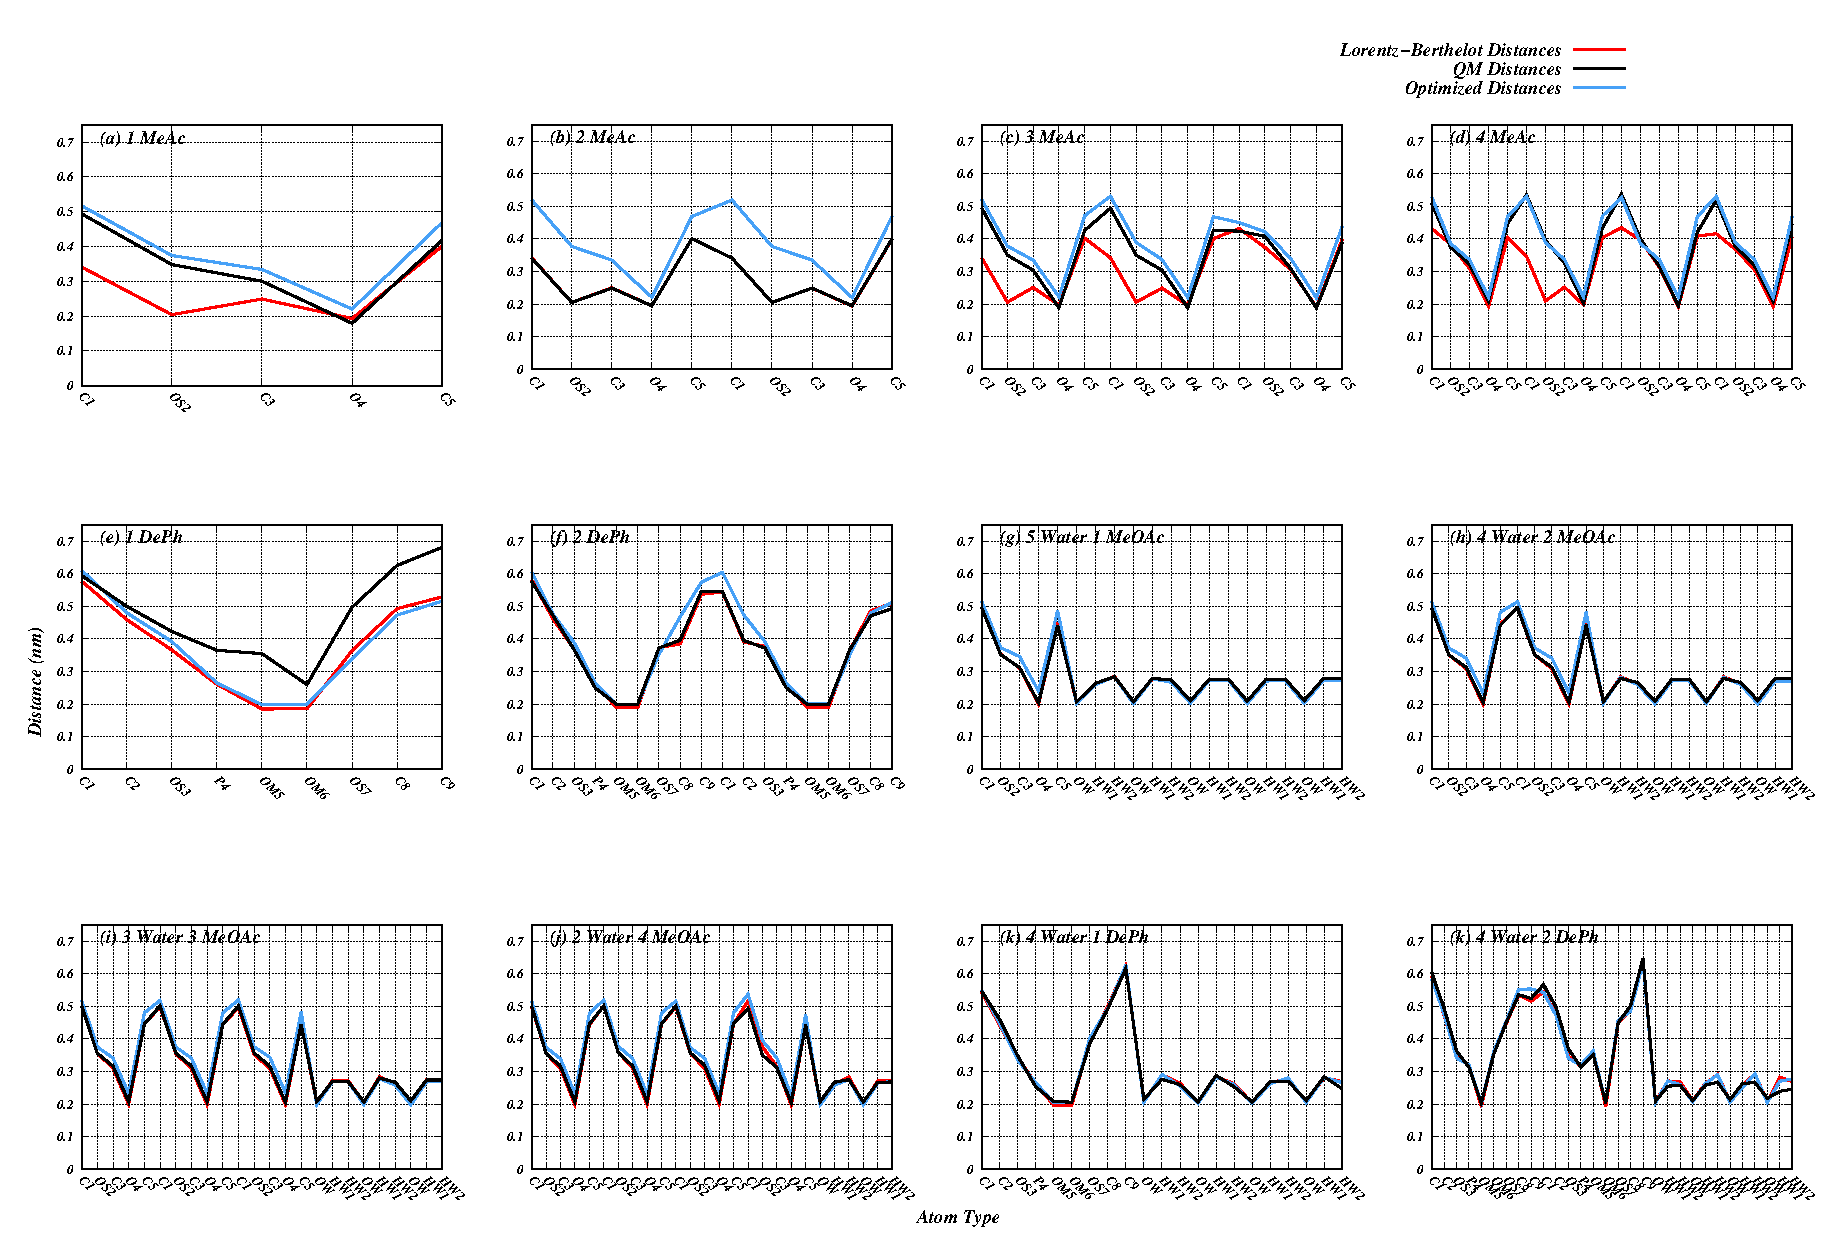
\includegraphics[width=\textwidth]{Figure_S1.eps}
\end{figure}

\begin{figure}
    \caption[Geometries of \li{} clusters with ligands]{Distances of all ligand atoms from \li{} for each cluster. 
    Lorentz--Berthelot parameters give geometries close to the target data, while the optimized parameters
    bring the ion slightly closer to electronegative oxygens.}
    \label{figch3:distances}
    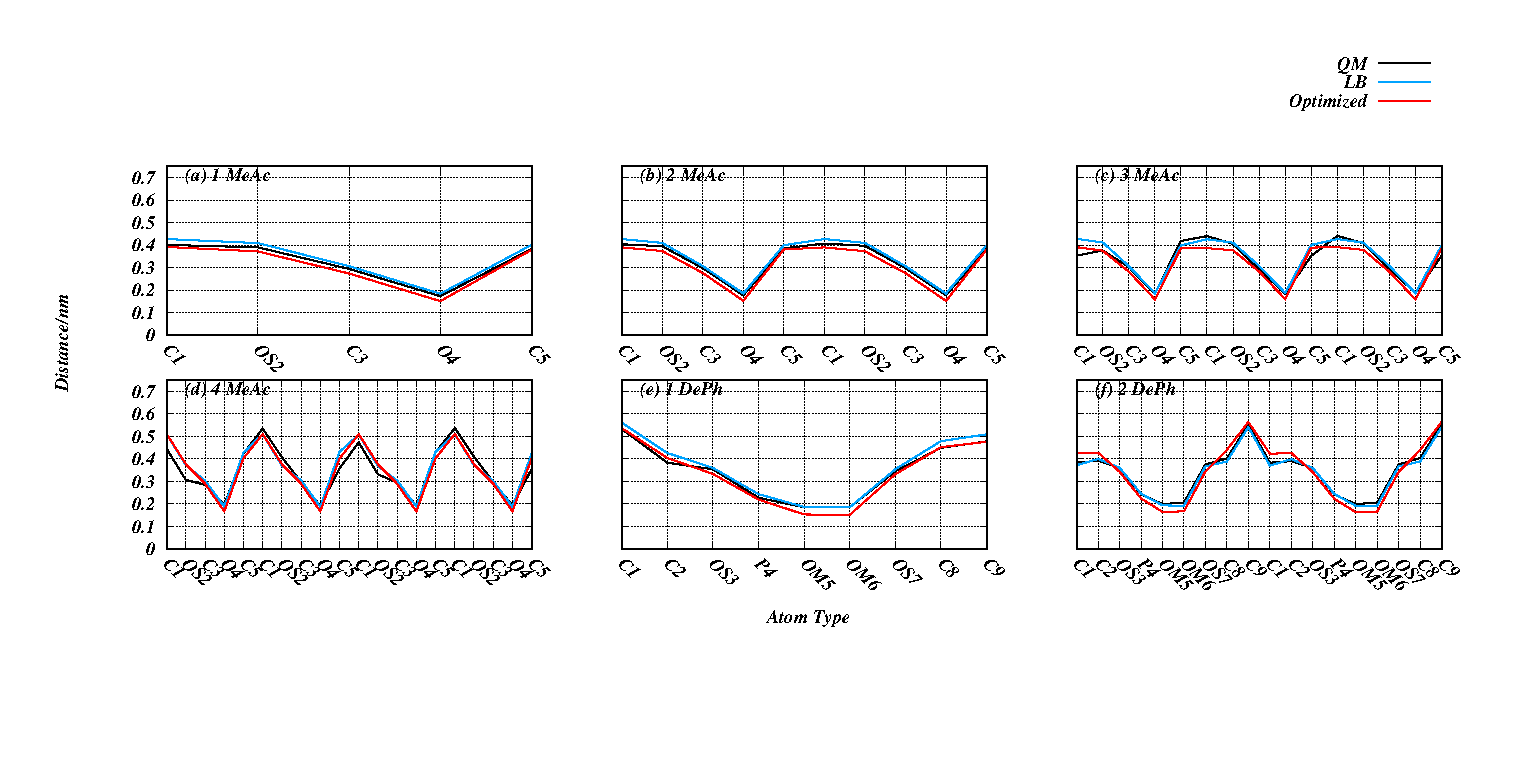
\includegraphics[width=\textwidth]{Figure_S2.eps}
\end{figure}

Describing the interactions of \mg with water presents several challenges, and there are numerous
models developed to describe \mg--water interaction~\cite{merzparams,villaparams,microparams}.
These models are optimized to improve the hydration free energies as well as
binding energies with various solvent models~\cite{merzparams,villaparams,microparams}.  
Previous work by our group has examined \mg models
from Li \etal{} and Allner \etal{}~\cite{merzparams,villaparams} in simulations with POPC lipids~\cite{kruczek:2019}, 
and found little variation among them in terms of their effects on lipid bilayer properties. 
With this in mind, we chose to focus our work here on the parameters developed by Li \etal{} because
their optimization procedures closely follow our focus on binding energies.
In recent work it has been reported that the existing \mg parameters, 
including those developed by Li \etal{}
overestimate the residence time for a water molecule in the 
first coordination shell of an ion~\cite{microparams}. 
In our past works using this force-field we reported 
insignificant Langmuir type adsorption of \mg ions to the POPC bilayer,
with waters retained in the first coordination shell of the ion~\cite{kruczek:2019}. 
We have also performed simulations with the parameters developed by Grotz \etal{} that directly
reduce residence times while not significantly changing other solvation 
properties of the ion~\cite{grotz:2021:optimized,microparams}. 
This was done to study how the interactions with water
could affect the first-shell coordination of \mg in the bilayer interface. 
We have {computed} 
the interaction cross-term for the \mg ion from Grotz \etal{}
with SPC/E water explicitly, using {the Lorentz-Berthelot mixing rules.}
Similarly to \li{}, we selected LJ cross-terms for use in our simulation following the procedure from Saunders \etal{} 2022~\cite{saunders:2022}. Target QM data for clusters of water with \mg are shown in table~\ref{tabch3:ionwater}.
\begin{table}[H]
    \centering
    \tiny
    \begin{tabularx}{\textwidth}{X|X|X|X|X|X|X}
        \hline
        Waters & CCSD(T)/CBS~\cite{wineman:2020:transferable} & PBE0+vdW~\cite{wineman:2020:transferable} & AMOEBA-HFC~\cite{wineman:2020:transferable} & Li et al.~\cite{merzparams} & Grotz et al.~\cite{microparams}  & Allner \etal{} \cite{villaparams}\\
        \hline
             1  &  -344.8  &  -349.9  &  -349.8  &  -276.8  & -282.8   &-270.3\\
             2  &  -651.0  &  -657.6  &  -657.3  &  -544.3  & -557.3   &-531.5\\
             3  &  -898.7  &  -904.6  &  -902.5  &  -792.1. & -815.2   &-774.3\\
             4  & -1101.2  & -1103.4  & -1100.4  & -1018.3 & -1055.3   &-995.7\\
        MAE &     -        &  4.9       &  4.0        &  91.1     &  71.3& 106.0     \\
        \hline
    \end{tabularx}
        \caption[\mg binding energies to water]{Mg$^{2+}$ binding energies to water clusters determined using different QM
    theories and classical force fields. All energies are in kJ/mol. These are used when
    computing the energies of substitution from water to lipid parts, which we use
    as our optimization target when selecting LJ cross-terms.}
    \label{tabch3:ionwater}
\end{table}
These energies for water were similar enough across force-fields that we chose to use only the values from Li \etal{}~\cite{merzparams} for use in computing substitution energies for our target data.
The result of our parameter search are shown in table~\ref{tabch3:params}.
\begin{table}
\tiny{
    \begin{tabularx}{\textwidth}{|X|X|X|X|X|X|X|X|X|X|X|}\hline
        \multirow{3}{*}{Atom type} & \multicolumn{4}{c|}{\li{}} & \multicolumn{6}{c|}{\mg} \\\cline{2-11}
                  &\multicolumn{2}{c|}{LB-Rules}&\multicolumn{2}{c|}{\mbnbfix}&\multicolumn{2}{c|}{LB-Rules}&\multicolumn{2}{c|}{\mbnbfix}&\multicolumn{2}{c|}{\mbnbfixmicro}\\\cline{2-11}
                  & \eps  & \sig  & \eps & \sig & \eps& \sig & \eps& \sig & \eps& \sig \\\hline
            CH3   & 1.07485 & 0.25797 & 0.99872 & 0.30898 & 0.19239 & 0.30856 & 0.68709 & 0.14257& 0.68709 & 0.14257\\\hline
            CH2   & 0.75411 & 0.27432 & 1.05729 & 0.20001 & 0.13238 & 0.32468 & 0.63126 & 0.20617& 0.63126 & 0.20617\\\hline
            OA    & 1.09408 & 0.21821 & 2.91925 & 0.20020 & 0.19044 & 0.26890 & 5.05190 & 0.26223& 5.05190 & 0.26223\\\hline
            P     & 1.85667 & 0.23975 & 6.99324 & 0.21844 & 0.32318 & 0.29044 & 3.89200 & 0.27811& 3.89200 & 0.27811\\\hline
            OM*   & 1.19328 & 0.21400 & 0.23749 & 0.20015 & 0.20771 & 0.26469 & 3.22262 & 0.17691& 3.22262 & 0.17691\\\hline
            CO*   & 0.35344 & 0.29727 & 0.48204 & 0.35920 & 0.06152 & 0.34796 & 0.56152 & 0.37127& 0.56152 & 0.37127\\\hline
            O*    & 1.19328 & 0.21400 & 0.06248 & 0.20068 & 0.20771 & 0.26469 & 2.43058 & 0.13069& 2.43058 & 0.13069\\\hline
            OW    & 0.95709 & 0.22875 & 0.95709 & 0.22875 & 0.16659 & 0.27944 & 0.16659 & 0.27944& 13.75000& 0.21010\\\hline
    \end{tabularx}}
    \caption[Lennard-Jones cross-terms for \mg]{Lennard-Jones cross-terms used in each \mg simulation. We have computed LB-terms using Lorentz-Berthelot (LB) mixing rules,
    starting with the self-terms for \li{} from Joung and Chetatham III\etal{}~\cite{joung:2008} and the self terms from \mg from the work of
    Li \etal{} ~\cite{merzparams}. The \mbnbfix parameters are chosen following the method described in section~\ref{sec:params}.
    The \mbnbfixmicro parameters for \mg only change the cross-term for OW-\mg, and were computed using LB-rules to mix the self-terms from
    Grotz \etal{}~\cite{microparams} with those of SPC/E water, without changing the cross-terms with anything else in the system. \eps~are in
    units of / Kj/mol and \sig~are presented in units of /nm.}
    \label{tabch3:params}
\end{table}
\section{Results and Discussion}
\subsection{Bilayer simulations of \li{} and \mg{}}
\subsubsection{Lipid bilayer structure}
% \paragraph{Densities}
The distribution of electron dense and heavy atoms is often studied by using
scattering techniques, like small-angle x-ray and neutron scattering. 
These methods
yield a scattering form-factor.  Densities can be obtained from the form-factor by solving
the inverse problem, which is a technically hard problem. In experiments this is usually solved by fitting a model to the form-factor.
Simulations give us direct access to atomic positions, and consequently
the densities. This allows us to compute a scattering form-factor by taking a cosine transform of the density{. The computed
form-factor}
can be compared with the direct measurements of the experiment.
The simulated lipid bilayer x-ray scattering form-factors and associated 
electron densities for each system are shown in figure~\ref{figch3:eledens}.
\begin{figure}[h!tb]
    \caption[Comparison of SAXS formfactors]{Comparison of x-ray scattering formfactors (a,b) and associated electron densities (c,d) for simulated systems. 
    {The system with \li{}{} salt has a slightly thicker bilayer compared to \na and the simulation without salt (a,c) and},
    \mg does not significantly change the bilayer thickness
    under any parameter set studied (b,d). }
    \label{figch3:eledens}
    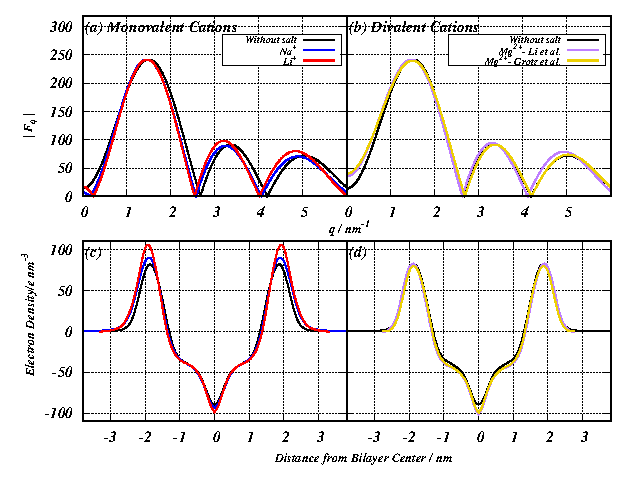
\includegraphics[height=0.3\textheight]{Figure_1.eps}
\end{figure}
We compare all form-factors for each system to that of a system simulated without salt, published
in our previous work~\cite{kruczek:2017}.
The bilayer thickness \dhh~is determined by measuring the distance between the
peaks in the electron density, which roughly localize the electron-dense phosphates in the
lipid headgroup -- the values for this can be seen in table~\ref{tabch3:struc}.
\begin{table}
    \caption[Bilayer simulation details and structure]{Bilayer simulation details, and structural parameters. Here we detail the various
    structural measurements of each simulated bilayer.
    \dhh~ is the distance measured between the peaks in the electron density, which localize the electron-dense phosphate moiety in the lipid headgroup.
    \db~ is a distance between the Gibb's surfaces{\cite{fogarty:2015}} on the probability density of solvent as it approaches the lipid bilayer.
    \dc~ is the distance between the Gibb's surfaces on the probability density of lipid chains, and represents the lipid chain thickness.
    Volume per lipid \vl~ is measured by dividing the volume of the entire system into solvent and ions, and lipid following the method by Petrache \etal{}
    {\cite{petrache:1997}}.
    This \vl~ is the sum of the \vh~ and V\textsubscript{C}, which are the volume per lipid headgroup and volume per lipid chains respectively.
    Area per lipid molecule \al~ is computed as the ratio of twice the lipid chain volume \vc~ with \dc. We also report the
position of the hydration boundary of each system, which we compute as the point where the second water order parameter $P_2(cos(\beta))\approx 0$
{as was done in Saunders \etal{} 2019~\cite{saunders:2019}}.}
    \label{tabch3:struc}
    {\tiny
    \begin{tabularx}{\textwidth}{Y|Y|Y|Y|Y|Y}
            &No Salt&\na&\li{}&\mgmbnbfix&\mgmicro\\\hline
        \dhh (nm)    &3.744   $\pm$ 0.107  &3.764   $\pm$ 0.088 &3.864  $\pm$ 0.070&3.832  $\pm$ 0.364  &3.768  $\pm$ 0.525\\
        \db  (nm)    &3.654   $\pm$ 0.047  &3.936   $\pm$ 0.043 &4.511  $\pm$ 0.048&4.325  $\pm$ 0.044  &4.213  $\pm$ 0.049\\
        \dc  (nm)    &2.707   $\pm$ 0.034  &2.897   $\pm$ 0.034 &3.015  $\pm$ 0.034&2.880  $\pm$ 0.029  &2.809  $\pm$ 0.032\\
        \vl  ($\times 10^{-3}\text{nm}^3$)&1215.57 $\pm$ 1.0   &1211.32 $\pm$ 1.21 &1201.2 $\pm$ 1.05&1219.8 $\pm$ 1.24  &1227.7 $\pm$ 1.24\\
        \vh  ($\times 10^{-3}\text{nm}^3$)&310.68  $\pm$ 1.14  &314.81  $\pm$ 0.75 &306.0  $\pm$ 1.01&324.0  $\pm$ 1.26  &327.9  $\pm$ 1.10\\
        \vc  ($\times 10^{-3}\text{nm}^3$)&904.89  $\pm$ 1.28  &896.50  $\pm$ 1.19 &895.3  $\pm$ 0.91&895.8  $\pm$ 1.05  &899.8  $\pm$ 1.06\\
        \al  ($\times 10^{-2}\text{nm}^2$)&66.86   $\pm$ 0.85  &61.89   $\pm$ 0.73 &59.39  $\pm$ 0.69&62.21  $\pm$ 0.63  &64.35  $\pm$ 0.82\\
        Hydration Boundary (nm) & 2.79 &3.69&3.63 &3.48&3.33  \\
\end{tabularx}}
\end{table}

Experiments often report various types of thicknesses, volumes, and cross-sectional areas that are model dependent.
We also compute these quantities to compare the simulation results with experiments. These values are presented in 
table~\ref{tabch3:struc}.
Based on the \dhh~and the \dc~ there is a slight thickening 
of the bilayer in the \li{} {simulation} above that seen in the \na {simulation}.
The \mg simulations {, irrespective of the parameter set, yield} much less thickening than {the}  
Li\textsuperscript{+} {simulation.} 
{The volumes per lipid (\vl), headgroup (\vh), and chains (\vc) are computed using the method of
Petrache \etal{}~\cite{petrache:1997}. This is done by optimizing the function:
\begin{equation}
    \label{eq:volumeobj}
    \Omega(v_i)=\sum^{\rho_s}_{z_j}(1-\sum^{N_{\text{Groups}}}_{i=1}{(\rho_i(z_j)v_i)^2})\text{,}
\end{equation}
where $\rho_i(z_j)$ is the number density of the $i$ component in the
$z_j$ slice of the box and $v_i$ is the corresponding partial component volume. $N_\text{Groups}$ is the number
of atom groups for which we are dividing the system volume into component volumes -- we have groups for solvent plus ions,
lipid chain without the terminal methyls (CH\textsubscript{*}), terminal methyls (CH\textsubscript{3}), and the lipid headgroups (H).
The lipid volumes are then computed as 
\begin{equation}
    \text{\vc}=N_{\text{CH}_*} \times v_{\text{CH}_*}+N_{\text{CH}_3} \times v_{\text{CH\textsubscript{3}}}
\end{equation}
and
\begin{equation}
    \text{\vh}=N_{H} \times v_{\text{headgroup}}\text{,}
\end{equation}
where $N_{\text{CH}_*}=30$, $N_{\text{CH}_3}=2$, $N_{\text{H}}=20$ are the number of united atoms per atom group for CH\textsubscript{*},
CH\textsubscript{3}, and H.
}{
The chain volume \vc~ is similar for all systems studied, and there is some variation in the headgroup volume \vh~.
However, this method of dividing up the volume is more prone to errors in the headgroup region due to 
significant overlap between the headgroup and solvent densities. 
Thus, we also see similar variation in the total lipid volume \vl. 
}
The two-dimensional area per lipid \al~is defined as
{$\frac{2V_c}{2D_c}$ as is often reported from SAXS and SANS experiments~\cite{nagle:2000}, and is an important
measure of how the lipids condense as the bilayer thickens.}
{Both the simulations with \mg yield bilayers with a larger \al~ 
    than the monovalent ions studied in this work, and are closer
in area to the simulation without salt.
}

The detailed structure of molecules and their neighborhoods are often studied using 
various nuclear magnetic resonance (NMR) techniques.
{At present, these experiments with various salts are sparse.}
{Thus,} we report these data with anticipation that future experiments will fill this gap and validate
or invalidate
these numbers.
Lipid chain ordering is determined via the acyl chain $S_{CD}$ per carbon
atom. These can be seen in figure~\ref{figch3:op}. 
\begin{figure}[h!tb]
    \caption[Acyl chain order parameters]{Acyl chain carbon-deuterium order parameters. These are computed for the Sn1 and Sn2 chains of each lipid starting at the 
        second carbon in the chain\cite{egberts:1988,Douliez:1995}. We note that the lipids simulated in systems of monovalent ions (a,c) show a significant increase
in the lipid chain ordering for both acyl chains. The systems simulated with \mg (b,d) are much closer in ordering to that of a system
simulated without ions.}
    \label{figch3:op}
    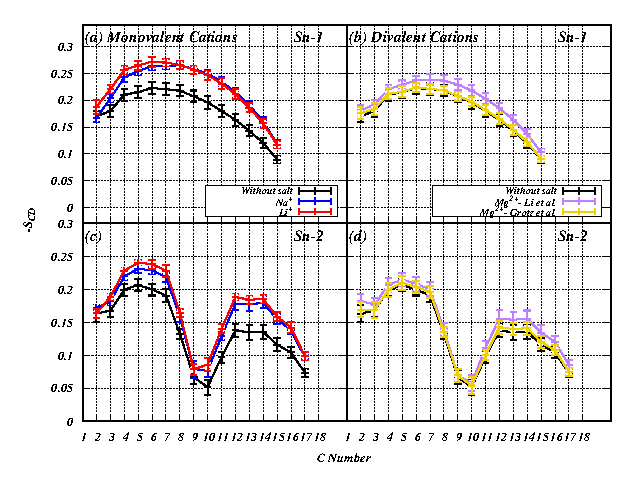
\includegraphics{Figure_2.eps}
\end{figure}

There is significant increase in chain ordering in the systems 
with \na and Li\textsuperscript{+}, which {is} consistent with the slight thickening
of the bilayer seen in the \db~ values. The less coordinated \mg systems have remained much closer to the 
ordering seen in the no-salt simulation.


\section{Specific ion adsorption}
\subsection{Bulk ions}

Interfaces in salt solutions give rise to a double layer of cations and anions at the surface~\cite{israelachvili:2011:intermol}. 
Ions in these double layers get stuck to the surface, or adsorb, which is sometimes referred to as specific binding. Zwitterionic lipid bilayers have no net charge before ions are adsorbed,
so this adsorption
determines the surface charge density on the substrate. This charge is measured experimentally using the electrophoretic mobility of the vesicle. Interpretation
of such experiments requires one to define a surface, often called the ``slip-surface'' where solvent 
beyond that point
can be represented by a dielectric continuum. The electrostatic potential at this surface is the $\zeta$--potential.
In simulations the interface is not a simple surface, but a region {without a clear point of delineation}. 

\subsubsection{Hydration boundary}
We {identify} this 
slip-surface boundary as the point where 
water orientational ordering is negligible, i.e.
beyond the ``slip-surface'' 
boundary water {quadrupoles} are {sufficiently isotropic,
giving dielectric properties of water similar to that of bulk solvent}.
We compute this by first dividing the box into 
slices along the direction normal to the bilayer. 
For each water within a slice we 
compute the average value of first and second order legendre polynomial of 
the cosine of the angle between the box z-axis and
the water O-H bond vector, and then average these values over the last 150 ns of simulated time.
Figure~\ref{figch3:h2order}~shows the water order parameters 
as a function of the distance of a slice from the bilayer center.
\begin{figure}[h!tb]
    \caption[Water orientational order parameters]{Water order parameters.   
        {The P1 and P2 calculated for monovalent cations (a,c) show greater 
            organization in the bulk region and the B\textsubscript{-2} regions, and less organization within 
            the lipid-occupied regions of the system (B\textsubscript{+} and B\textsubscript{-1}) compared to the simulation without salt. 
        } 
{On the other hand, with the presence of \mg salts we observe an overall less pronounced effect in the
bulk and B\textsubscript{-2} regions compared to the system without salt (b,d).}
}
    
    \label{figch3:h2order}
    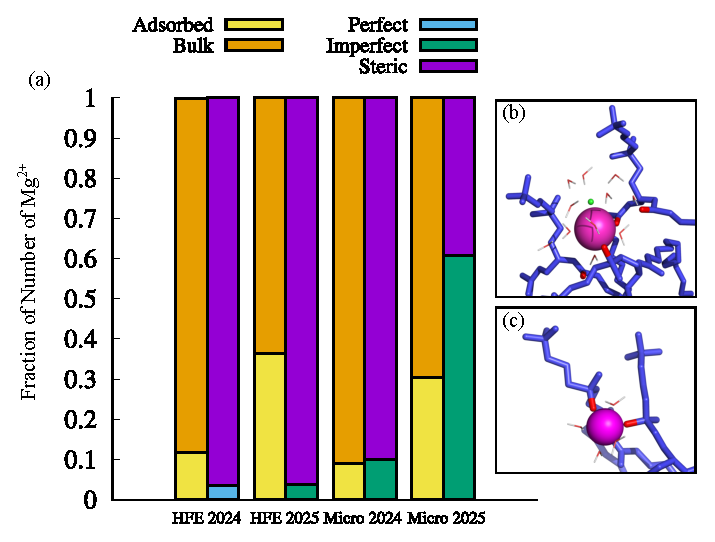
\includegraphics[width=0.5\textwidth]{Figure_3.eps}
\end{figure}

The first order parameter describes the in-out ordering of the bond vector with respect to the 
box z-axis -- a vector parallel to the axis and pointing normal to the bilayer would have a positive
ordering, and a vector pointing into the bilayer would have a negative ordering. We see that waters at the surface
of each bilayer have a significant outward orientation at the bilayer surface, and that reverses as we move
closer to the bilayer center. When compared to the system simulated without ions, we see that
the monovalent ions perturb the water in-out orientation 
more than Mg\textsuperscript{2+}, especially in the case of the \mgmicro
parameters.

The second order parameter
roughly describes the organization of the quadrupole moments of water, {and the value of this parameter
can be used to compute the} quadrupolar splitting values determined in 
deuterated water NMR experiments~\cite{aaman:2003,kruczek:2017:ether}.
The vertical dotted lines in figure~\ref{figch3:h2order} denote regions of interest in the bilayer 
based on the {sign} of the second order parameter. We call the innermost region of negative ordering
B$_{-1}$, which ends when the values become positive. This next region of positive ordering is
called B$_{+}$, and the following region of negative ordering is B$_{-2}$. Each bilayer system with ions
has these regions, but they are at differing distances from the bilayer center.
It should be noted that beyond the $B_{-2}$ region the ordering does not abruptly reach zero in the systems
simulated with salt.

{
    Figure~\ref{figch3:h2order} shows monovalent ions have 
    less organization in the B\textsubscript{-1} region (inside the lipid headgroup) when compared to that of the divalent ions,  
    whereas in regions B\textsubscript{+} and B\textsubscript{-2} (closer to the bilayer surface) the divalent ions show significantly
    less organization compared to that of monovalent salts.} 
The hydration boundary is determined by  
fitting an exponential decay to the second water order parameter starting
at the minimum of the B$_{-2}$ of the histogram.
The decay length is used to demarcate the point where the ordering becomes zero -- water beyond this region is
regarded as bulk solvent. The location of the hydration boundary 
is noted in figure~\ref{figch3:h2order}, and the distance 
to this point from the bilayer center is listed in table~\ref{tabch3:struc}.

\subsubsection{Poission-Boltzmann Theory}
With the boundary defined, we look to the region of bulk solvent to examine the behavior of ions and ascertain that
they follow the predictions of PB-theory\cite{israelachvili:2011:intermol}. 
The purpose of this endeavor is to distinguish the ions in bulk solvent from those that are adsorbed,
as the density of the adsorbed ions are expected to deviate from PB-theory predictions.
We must first compute all the model parameters for the number density and electrostatic potential predicted by
PB-theory, and compare our simulation results to this prediction.
The PB-theory assumes 
that the number density of ions follow a Boltzmann distribution:
\begin{equation}
    \rho(z) = \rho_0 \exp\big({- \bar z \text{\si{\elementarycharge}} \beta \psi(z)}\big)\text{,}
    \label{eq:gcnum}
\end{equation}
where $\rho_0$ is the ion density in the center of the dielectric continuum, $\bar z$ is the valency of the ion, 
$\beta = (k_bT)^{-1}$, \si{\elementarycharge} is the charge
on an electron, and $\psi(z)$ is the electrostatic potential. The surface is defined by the hydration boundary of each system. 
The lengths of the solvent occupied regions, $D$, {in each system is} found by measuring the distance across the solvent from the 
hydration boundary of one leaflet of the bilayer to the other. 
These values are listed in table~\ref{tabch3:gctheory}.
\begin{table}
    \caption[Poisson-boltzmann theory parameters]{Poisson-boltzmann theory parameters. These parameters are computed for each
    simulated system studied (excepting the bulk density $(\rho_{0,i})$, 
    which we fit to our simulation results). These are then used to compute the
    number density distribution and the electrostatic potential as described by 
    Poisson-Boltzmann theory to compare to our simulation results.
    \sig is the surface charge density of the bilayer, D is the length
    of the bulk-solvent occupied region of the box, K is the Debye
    screening length, and $\rho_{0,i}$ is the number density of the particular 
    ion at the center of bulk solvent.}
    \label{tabch3:gctheory}
    \begin{tabularx}{\textwidth}{|X|X|X|X|X|}\hline
        Parameter                    & \na  & \li{}    & \mgmbnbfix    & \mgmicro \\\hline
        \sig ($e/nm^{2}$)            &0.161 &0.182   &0.0690  &0.0476     \\\hline
        D~($nm$)                     &26.927&26.557  &26.658  &25.226     \\\hline
        K~($nm^{-1}$)                &3.331 &3.333   &3.913   &3.921      \\\hline
        $\rho_{0,cation}$~($nm^{-3})$&0.059 &0.060   &0.091   &0.092      \\\hline
        $\rho_{0,anion}$~($nm^{-3})$ &0.062 &0.063   &0.183   &0.185      \\\hline
    \end{tabularx}
\end{table}
This places the surfaces at $z=\pm D/2$~nm, where $z=0$ is the center of the solvent-occupied region of the simulation box.
The electrostatic potential $\psi(z)$ is modeled as a sum between two Debye-Huckle potentials~\cite{israelachvili:2011:intermol}:
\begin{align}
    &\psi_{1}(z) = \psi_s \exp\bigg({-K(z+\frac{D}{2})}\bigg)\\
    &\psi_{2}(z) = \psi_s \exp\bigg({K(z-\frac{D}{2})}\bigg)\\
    \label{eq:gcpot}
    &\psi(z) = \psi_1(z) + \psi_2(z) - \big({\psi_1(0)+\psi_2(0)}\big)\text{,}
\end{align}
where $\psi_s = \frac{\sigma}{\epsilon_0\epsilon} K$ is the electrostatic potential at the bilayer surface
as defined by the hydration boundary, $\epsilon$ 
is the dielectric constant of SPC/E water $\epsilon=70.7$~\cite{reddy:1989:dielectric}, and $\sigma$
is the surface charge density of the bilayer leaflet~\cite{israelachvili:2011:intermol}. 

$\sigma$ is determined for
each system by integrating the charge density of all species within the hydration boundary on either side of the bilayer.
This charge divided by the box area is the surface charge density.
These values can be seen in table~\ref{tabch3:gctheory}. {Since our
    phospholipid is zwitterionic, all of the surface charge comes from the
ions that have accumulated within 
the hydration boundary (see figure~\ref{figch3:dens})}
\begin{figure}[h!tb]
    \caption[Number densities]{Number density of lipid headgroup species and
    ions near the bilayer interface. (a-b) We report that the 
    monovalent cations show peaks near the phosphate, with
    accumulation of an anion peak that resembles the double layer.
    (c-d) \mg does not show significant accumulation in the 
    lipid bilayer headgroup compared to the monovalent ions,
    with a similarly small anion peak. However, in all systems
    studied, ions are accumulated near the phosphorus.
    Integrating the number density of cations within the hydration boundary,
    denoted by the purple vertical dashed line, gives the number of ions that are
    sterically bound. The orange vertical dashed line delineates the \dhh~and the 
    red vertical dashes
delineate the D\textsubscript{C}~of the bilayer.}
    \label{figch3:dens}
    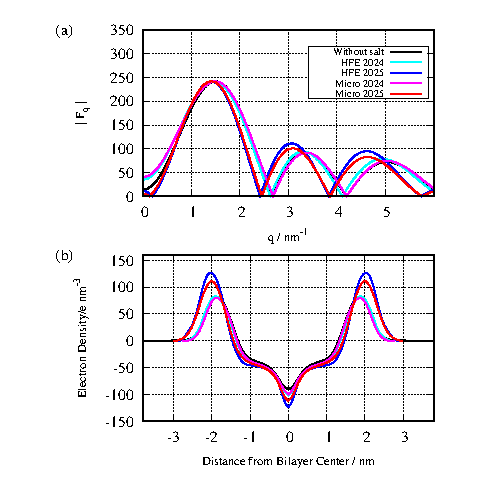
\includegraphics[width=\textwidth]{Figure_4.eps}
\end{figure}

Returning to equation~\ref{eq:gcpot}, $K$ is the inverse Debye length,
\begin{equation}
K=\sqrt{\sum_{i} \rho_{0,i} \bar z_i^2\frac{\text{\si{\elementarycharge}}^2}{\epsilon_0 \epsilon k_bT}},
\label{eq:debyelength}
\end{equation}
where $\rho_{0,i}$ is the density of each ion in a given system at the center of bulk solvent.
This is taken as an average of the number density of each ion in the solvent occupied region of the box.

Finally, we fit equation~\ref{eq:gcnum} to the density of anions in 
bulk solvent via $\rho_0$. The comparisons
can be seen in figure \ref{figch3:catgcdens}.
\begin{figure}[h!tb]
    \caption[Number densities of cations and anions]{Number density of cations and anions in the bulk solvent-occupied region of each
    simulated system, compared with theoretical predictions from PB-theory for each calculated $\sigma$. PB-theory predictions
    correspond well with the simulation results within the region bounded by the hydration boundary.}
    \label{figch3:catgcdens}
    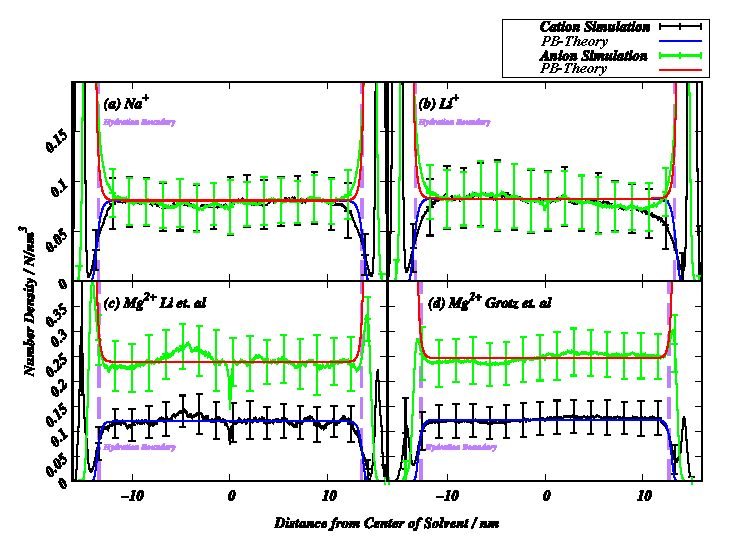
\includegraphics[width=\textwidth]{Figure_5.eps}
\end{figure}
Past the hydration boundary of the lipid bilayer, it can be seen that the density of anions continues 
to climb monotonically. Additionally, the density of cations 
drops monotonically to a trough value before climbing closer to the bilayer center, near the phosphate groups 
(see figure \ref{figch3:dens} and \ref{figch3:catgcdens}). 


We also compare {the} 
electrostatic potential from our simulations 
to the potential from PB-theory 
(figure \ref{figch3:potgc}). 
\begin{figure}[h!tb]
    \caption[Electrostatic potential]{Electrostatic potential in the bulk solvent-occupied region compared to predictions from PB-theory. We report good
    agreement between the theoretical potential shown in green, and the simulation results shown in black, within the region bounded by the hydration
    bounds of the lipid bilayer.}
    \label{figch3:potgc}
    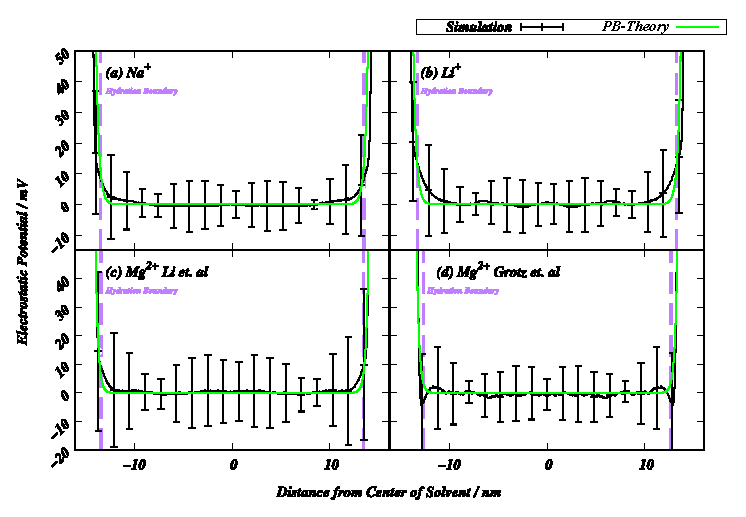
\includegraphics[width=\textwidth]{Figure_6.eps}
\end{figure}
The electrostatic potential for each simulated system can be computed 
by twice integrating the Poisson equation 
\begin{equation}
    \phi(z)=-\frac{1}{\epsilon_0}\int_{0}^{z}\int_{0}^{z'}\rho(z) dz dz' + C_1z + C_2\text{.}
    \label{eq:poissonint}
\end{equation}
We set the boundary conditions that
the electric field in bulk solvent must be zero, and the electrostatic potential at the box edge must be zero.
The electrostatic potential from simulation agrees well with the prediction from PB-theory.


\subsection{Adsorbed ions}
\label{sec:boundions}
The total number of adsorbed ions are counted as the number of ions within the ``slip-surface'' or ``hydration-boundary'' of the bilayer, and
further characterization is based on the level of hydration of the ion.
Binding constants from the Langmuir Isotherm model are often computed in experiments to describe ion binding affinity for
surfaces; however, this model requires a fixed number of binding sites per lipid. The actual number of binding sites
per lipid is not known. Therefore, we report the number of ions adsorbed per lipid $(\theta)$, which 
{is related to} 
the binding affinity of each ion for the lipid bilayer.
We observe 0.51 \na per lipid bound, 0.57 \li{} per lipid, 0.13 \mg per lipid in the \mgmbnbfix system, and 0.10 \mg per lipid
in the \mgmicro system. We see a substantially larger number of \na and \li{} adsorbed per lipid than
\mg, which may be reflective of the amount of space occupied by each ion, and seems to follow the
binding modes such that the more dehydrated ions correlate with a larger number of ions adsorbed per lipid.
The fraction of cations adsorbed in each mode of adsorption can be seen in table~\ref{tabch3:cationfrac}, and the fractions
of \cl anions adsorbed can be seen in table~\ref{tabch3:anionfrac}.
\begin{table}
    \caption[Fractions per lipid of cations per adsorption mode]{Fractions per lipid of cations perfectly adsorbed, imperfectly adsorbed, sterically adsorbed, and non-adsorbed cations
        {averaged over the last 150~ns of simulation time}. These are computed
    by counting the number of waters in the first-coordination shell of every ion in the simulation box in every frame. For the total number
    of adsorbed ions, we
    only check if the ion is within the hydration boundary of the bilayer. We then subtract the number within this region that are
    completely dehydrated -- these are the perfectly adsorbed ions. We further subtract any ions that have lost 
    one or more waters -- the imperfectly adsorbed
    ions. The remaining are considered sterically adsorbed. 
    We also report the total number of bound ions per lipid as a measure 
    of the affinity of the ion to the lipid bilayer -- the number of \mg
    ions per lipid is fall smaller than that for the more perfectly adsorbed ions \li{} and Na\textsuperscript{+}.}
    \label{tabch3:cationfrac}
    \begin{tabularx}{\textwidth}{|X|X|X|X|X|}\hline
    Adsorbed cations / lipid & \na & \li{} & \mgmbnbfix   & \mgmicro \\\hline
    Total     $\theta$       &{0.472}&{0.575}&{0.129}&{0.091}     \\\hline
    Steric    $\theta_s$     &{0.010}&{0.015}&{0.116}&{0.071}     \\\hline
    Imperfect $\theta_I$     &{0.068}&{0.165}&{0.008}&{0.020}     \\\hline
    Perfect   $\theta_P$     &{0.394}&{0.395}&{0.005}&{0.000}     \\\hline
    \end{tabularx}
\end{table}
\begin{table}
    \caption[Fractions per lipid of anions per adsorption modality]{Fractions per lipid of anions perfectly adsorbed, imperfectly adsorbed, sterically adsorbed, and non-adsorbed anions in each simulation, defined in the same way as we define
    adsorption of cations. These are computed
    by counting the number of waters in the first-coordination shell of every anion in the simulation box in every frame. For the total number
    of adsorbed anions, we
    only check if the anion is within the hydration boundary of the bilayer. We then subtract the number within this region that are
    completely dehydrated -- these are the perfectly adsorbed anions. We futher subtract any ions that have lost
    one or more waters -- the imperfectly adsorbed
    ions. The remaining are considered sterically adsorbed. We indicate each system by the cation name, as the anion in the system is always Cl\textsuperscript{-}.
    We note that the anion binding fractions follow the trend seen in the total number of cations bound for each system, due to the formation of the ionic double-layer
    at the bilayer-water interface.
    Most anions adsorb sterically in each system, with some adsorbing imperfectly as they approach the positively charged choline trimethylammonium in the lipid headgroup.}
    \label{tabch3:anionfrac}\tiny
    \begin{tabularx}{\textwidth}{|X|X|X|X|X|}\hline
    Adsorbed anions / lipid     & \cl in \na System & \cl in \li{} System & \cl in \mgmbnbfix System& \cl in \mgmicro System\\\hline
    Total      $\theta  $&0.423&0.463& 0.186&0.208 \\\hline
    Steric     $\theta_s$&0.209&0.213& 0.107&0.126 \\\hline
    Imperfect  $\theta_I$&0.214&0.250& 0.079&0.082 \\\hline
    Perfect    $\theta_P$&0.000&0.000&  0.0 & 0.0  \\\hline

    \end{tabularx}
\end{table}
\cl adsorption fractions follow a similar trend to that of the total number of cations bound, but adsorption
is almost entirely in the steric modality.




\subsubsection{Adsorption modalities}

% The total number of adsorbed ions can be seen in~\ref{tabch3:struc}.
Further characterization of the adsorbed ions begins by examining the first-shell coordination partners of cations in each system.
This can be counted by first determining a cutoff value for the first hydration shell of each ion 
-- the values for this cutoff are
3.2~\AA~for Na\textsuperscript{+}, 2.7~\AA~for Li\textsuperscript{+}, 3.3~\AA~for Mg\textsuperscript{2+}, 
and 3.0~\AA~for Cl\textsuperscript{-}. 
These values are determined from radial distribution 
functions for water oxygen (or water hydrogen in the case of \cl) around each. 
This cutoff is used to produce a neighborlist for ions
across each simulation in every frame, and count the number of neighbors within this cutoff. 
These data {are} histogrammed and averaged over
the last 150ns of simulation time. The results for this are presented in figure~\ref{figch3:cood}.
\begin{figure}[h!tb]
    \caption[First shell coordinators for \li{} and \mg]{First shell coordination partners 
        for \li{} and \mg in each simulation. 
        These are computed over the last 150ns of 
        simulation time in each system by counting 
        the atoms of each species within a cutoff 
        of each ion in the system, and histogramming 
        the data based on the position of the ion. 
        The dotted vertical lines denote the various 
        bilayer surfaces -- the vertical black
        line delineates the hydration boundary of the bilayer,
        the vertical blue line delineates the D\textsubscript{HH},
        and the vertical red line delineates the D\textsubscript{C}.
        \li{} (a) retains some water 
        coordination well into the bilayer
        interface.
        \mgmbnbfix (b) on the other hand does not lose
        nearly any first-shell coordinating
        waters in the bilayer, with some exchange for phosphate
        oxygens. The \mgmicro (c) parameters yield again more exchange but 
        relatively far less than the monovalent
    ions.}
    \label{figch3:cood}
    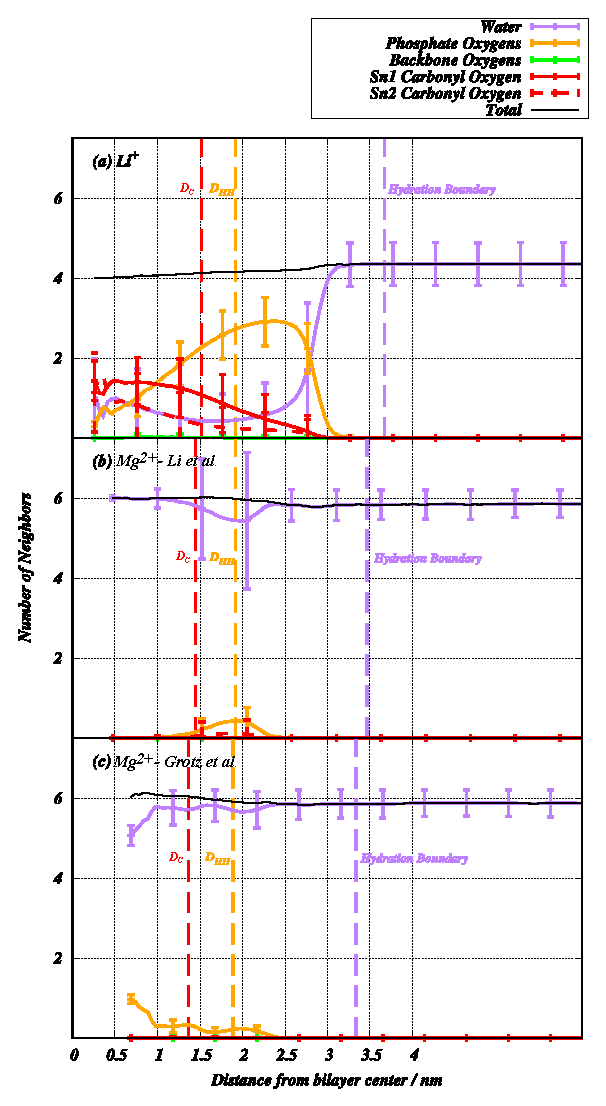
\includegraphics[height=0.7\textheight]{Figure_7.eps}
\end{figure}

The number of perfectly adsorbed ions is determined by counting the number of ions without any remaining 
waters in their first coordination shell. It is observed that in the \na system, a 
majority of the ions adsorbed to the bilayer are completely dehydrated. %(see table~\ref{tabch3:cationfrac}). 
The \li{} system has a similar fraction of perfectly adsorbed ions compared to Na\textsuperscript{+}, 
and practically no perfectly adsorbed 
ions are seen in any of the \mg simulations. \cl anions are not seen adsorbed perfectly in any simulation.

Similarly to the perfect adsorption case, imperfectly adsorbed ions are counted as ions with one or more waters in their 
first coordination shell, but missing at least one
water from the shell. {We use the number of coordinating waters of an ion in the bulk solvent region
    of our simulation as the maximum coordination number for the ion (Figure 7). This
gives a coordination number of 4 for \li{} and 6 for 
Mg\textsuperscript{2+}.} We calculate 
{the number of imperfectly adsorbed ions} by counting the number of ions with 
one or more water missing from their hydration shell, and then subtracting the number of perfectly adsorbed ions.
We see more than twice the fraction of these ions in the \li{} system compared to the \na system. \mg shows an insignificant
number of imperfectly adsorbed ions. \cl adsorbs in a large fraction imperfectly, as they begin to interact with the headgroup trimethylammonium.

The remaining ions are considered sterically adsorbed -- this number is whatever ions remain after subtracting the 
perfect and imperfectly adsorbed ions from the number of overall adsorbed ions based on the position of the hydration boundary. 
\mg seems to have most of the ions in this adsorption mode, where \na and \li{} do not 
adsorb in this way in significant numbers. Additionally, \cl shows significant steric adsorption.

These data raise the question, what determines the mode of adsorption for a given ion? Since everything else, such as
the substrate and the solvent, are held constant, the magnitude of the electric field at the position of the hydration shell
of each ion is all that remains to determine the adsorption modality of the ion (figure~\ref{figch3:cationfrac}).
\begin{figure}[h!tb]
    \caption[Fractions of ion-adsorption modalities]{Fractions of ion-adsorption modality per each simulated system as a function of electric field strength. Here we 
    show that the fractions of ions adsorbed in each modality follow a trend with an increasing electric field strength at the
    hydration shell of the cation. The overall trend is that the cations with the weakest field at the hydration shell position
    adsorb more perfectly, and as the field strength increases more ions adsorb imperfectly and then sterically. We note
    that little correlation with field strength can be seen in the total number adsorbed per ion.}
    \label{figch3:cationfrac}
    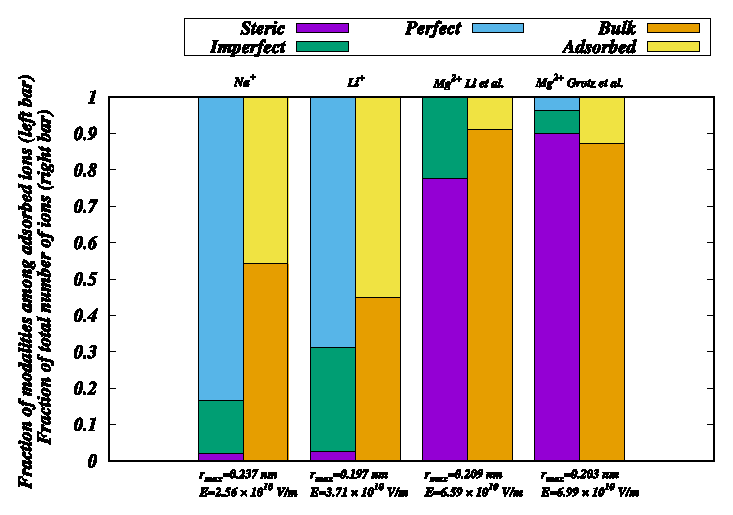
\includegraphics{Figure_8.eps}
\end{figure}
The electric field strength of each ion is calculated by applying Coulomb's law to a point charge, placing the test charge at the 
position of the first hydration shell of the ion in question. We note that the \mgmbnbfix ion keeps waters slightly closer in the hydration shell
compared to the \mgmicro model{,}{resulting in} a stronger electric field 
produced at this point by that ion.
The largest ion with the smallest charge-density \na dehydrates completely in the largest fraction. \li{} is smaller, and thus the field near
the first shell is stronger and can hold waters a little better than \na. \mg is similar in size to \li{}, but has a 2+ charge and
holds onto waters substantially more than either of the monovalent ions.  
We also note that the $\norm{\vec{E}}$ does not exhibit strong correlation with the fraction of the total number of ions adsorbed in each system, it
only determines the adsorption mode. 

\section{Conclusions}
Ion adsorption to porous interfaces is a complex interplay 
between solvent--surface, solvent--ion, and solvent--solvent
interactions. With the solvent--surface and solvent--solvent interactions 
held constant, we identify
three different adsorption modalities of ions based on the degree of 
dehydration of the ion upon adsorption. 
The binding modality of a particular ion is significantly correlated 
with the electric field strength of the ion
at the position of the first hydration shell, with stronger fields 
encouraging less dehydration of the ion upon
adsorption to the surface {(figure 8)}. This affect appears irrespective of the force-field 
used in the case
of \mg, which primarily adsorbs in the non-Langmuir type steric modality.


Furthermore, we identify several bilayer structural
parameters that can be verified experimentally via x-ray scattering, neutron
scattering,
or various NMR methods {(figures 1, 2, and 3 respectively).}
While the effect on lipid bilayer structure is not obvious in
the electron density {(figure 1)}, the pertubation can be seen in the \db~and water density --
the less hydrated ions induce slight thickening of the lipid bilayer. This
is reinforced by the chain ordering, where these ions increase chain ordering {(figure 2)} 
while the hydrated ions leave the lipid bilayer structure similar to that of the no-salt case.
These two results can be verified experimentally via solvent deuterium NMR, and lipid chain NMR.
In the case of POPC, we expect deuterium solvent quadrupolar splitting values will be 
{larger} 
for the less hydrated ions \na and \li{} when compared to the more hydrated Mg\textsuperscript{2+} {(figure 3)}. 
We also expect the lipid chain order parameters to follow the opposite trend,
with the monovalent ions inducing more ordering and \mg inducing a smaller change from the no-salt system.
We also expect that the adsorption of \mg will be less detectable via the 
electrophoretic mobility of a vesicle in an MgCl salt solution, as
the energy required to remove a hydrated ion from 
beneath the slip-surface of a vesicle may be low enough to allow their escape, while a dehydrated ion may remain
adsorbed.
These experiments are needed to verify
these conclusions. 
\chapter[Alteration of Bilayer Structure by \mg{}]{Alteration of Bilayer Structure by \mg{}\footnote{Portions reprinted with permission from Matthew Saunders; Sagar A. Pandit; Sameer Varma.
Alteration of Lipid Bilayer Structure by Mg$^{2+}$.
\textit{Langmuir}, American Chemical Society, manuscript in review, 2025. See appendix~\ref{app:permissions3} for author contributions.}}
\graphicspath{{CH4/figures/}}

\section{Abstract}
Developing molecular mechanics force fields to model interactions of biological
membranes with \mg{} cations is challenging. There are no direct estimates of the
binding modes of \mg~ions with lipid headgroups or other phosphates in the condensed
phase. Experimental data on lipid bilayers in \mg{} solution are sparse and limited
to biologically relevant but very low ion concentrations. At these concentrations, no
statistically discernible effects on bilayer properties are observed.
Simulations at these concentrations are difficult due to system size and the extensive conformational
sampling required for force-field development.
Considering these issues, we previously calibrated \mg-lipid Lennard-Jones cross-terms
using benchmarked quantum mechanical (QM) target data on small clusters of ions and
ligands representative of common cation binding sites on 1-palmitoyl-2-
oleoyl-sn-glycero-phosphatidylcholine (POPC). Our
simulations with these new \mg{} parameters yielded bilayer structures very similar
to those without salt, in agreement with available experimental data. 
We adopted this strategy because it worked well for modeling
membrane interactions with monovalent cations, for which additional experimental
data are available. However, newer studies from our group show that for \mg~ions,
the choice of target \mg-lipid mimetic clusters is non-trivial. Inclusion of fully
coordinated (6-fold) \mg~ions, which better represent potential ion-lipid structures
in the condensed phase, may be critical for selecting models that reproduce
experimental condensed-phase interactions of \mg~with nucleotide phosphates.
Using this new protocol, we propose an additional set of \mg-lipid interaction
Lennard-Jones cross-terms. With this parameter set, we find that at concentrations 
between 100-200 mM, there is a systematic thickening of the lipid bilayer, not observed
with our previous \mg-lipid model. Additionally, compared to the earlier model, we
observe more \mg~adsorbed on the bilayer and a larger fraction directly
coordinating lipid headgroups. However, the new model does not alter our previous
observation that structural changes in the bilayer correlate with the amount of
ionic charge directly coordinating lipid molecules.


\section{Introduction}

Salts have a well characterized behavior at interfaces in the condensed phase -- ions form a classic double layer, where
one charge accumulates near the substrate's surface, and the second charge then accumulates to compensate for 
that charge~\cite{israelachvili:2011:intermol}.
This can be explained using a mean-field approximation. 
However, the mean-field approximation does not provide details on specific interactions between ionic species and 
interface moieties. These details are non-trivial, especially in the case of
phospholipid membranes, where the substrate itself is liquid and can adopt new conformations in response to ion adsorption. 

Molecular dynamics (MD) simulations can, in principle, provide such details. 
However, the development of MD force fields for \mg{}, and modeling their interaction with lipid bilayers poses significant challenges.
Firstly, experimental data needed for force field development and validation is scarce.
To our knowledge, there are no direct estimates on the binding modes of \mg~ions with lipid headgroups or any other phosphates in the condensed phase. 
Secondly, the effects of \mg{} on lipid bilayer structure are only known for small concentrations
of salt~\cite{kurakin:2022:cations,kurakin:2021:effect}.
Simulations such low salt concentrations push the limits of hardware requirements for conformational sampling and force field testing. 
For example, in our previous simulations with \na{}~\cite{saunders:2022}, we observed between 75-90 \na{} ions adsorbed to an equilibrated lipid bilayer of 
100 POPC molecules per leaflet. If we assume similar numbers of \mg to be adsorbed, 
simulating at a biologically relevant concentration of 0.5 mM~\cite{romani:1992:regulation} will require more than 11 million waters.
Additionally, since the residence time of waters in the first shell of \mg~is 
of the order of a microsecond \cite{neely:1970,Palinkas:1982,bleuzen:1997}, 
capturing statistics on water-lipid exchanges in the first shell of \mg~requires prohibitively long MD simulations. 

Considering these issues, we previously chose to calibrate \mg-lipid Lennard-Jones (LJ) terms using 
benchmarked quantum mechanical (QM) target data clusters of small molecules representative of the
ion binding sites on 1-palmitoyl-2-oleoyl-sn-glycero-phosphatidylcholine (POPC)~\cite{saunders:2022}. 
Methyl acetate (MeAc) and diethyl phosphate (DEPh) were taken as small molecule representatives for lipid headgroups, 
and we targeted the changes in energy and structure associated with replacing water molecules in \mg-water clusters with these smaller molecules.  
Using this model we found that at about 100 mM concentration, \mg adsorbed into the headgroup region of POPC bilayer, 
but without losing its inner-shell waters (steric binding mode). We also observed formation of ion double layer at the headgroup-water interface.
However, \mg~adsorption had a negligible effect on POPC bilayer structure. We posited that since our model at 
high salt did not affect bilayer structure, our model at low experimental salt concentration will also not affect POPC bilayer structure; making the result consistent with experiment. 
We adopted this strategy because we showed that it worked well for modeling interactions of lipid bilayers with monovalent cations \cite{saunders:2022}. Prior to our development, all simulations, irrespective of the employed force field, reported that monovalent salts thickened POPC bilayers \cite{sachs:2004,melcr:2018,jurkiewicz:2012,kruczek:2017}. 
In contrast, experiments reported insignificant changes in POPC lipid bilayer structure \cite{pabst:2007:rigidification,petrache:2006:swelling}. 
The use of our new \na-lipid LJ terms resolved this discrepancy to a large extent \cite{saunders:2022}. 
Recent developments in our lab, however, motivate us to explore a modified strategy for developing \mg-lipid LJ terms. 
Our recent work of polarizable force fields for describing \mg-protein/nucleotide interactions \cite{julian:2023:mg} suggests that perhaps within the classical framework, a single set of force field parameters for \mg do not perform well at simultaneously reproducing 
energies of both fully coordinated (6-fold)
and partially coordinated \mg~structures. 
Furthermore, force field developed using 6-fold coordinated structures performed excellently at reproducing not only local interactions of 
\mg~ions in clusters containing nucleotide phosphates but also condensed phase binding free energies of \mg~ions with nucleotides \cite{julian:2023:mg}. We have shown that this strategy also works for other cations \cite{JACS2025} 
Fully coordinated 6-fold clusters of \mg~were not considered in the development of our previous \mg{} model~\cite{saunders:2024}, in which target data consisted of only partially coordinated structures of \mg.

Here we apply this new protocol to develop a new set of \mg{}-lipid LJ
terms. Our target data consists exclusively of full 6-fold coordinated \mg~clusters with 
different combinations of waters and MeAc/DEPh ligands representative of the common binding sites on POPC.
This allows us to focus our model parametrization on clusters that are more representative of the dense, bulk phase systems that we are interested in studying. 
As before, target data are obtained from benchmarked quantum mechanical (QM) vdW-inclusive density functional theory (DFT).

Using these new parameters, we perform MD simulations of POPC in \mgcl{} solution with the aim of comparing these results
with those of our previous interaction model parameters. We also characterize their behavior using two different
ion-water interaction parameter sets, parameters from Grotz \etal~\cite{grotz:2021:optimized,micro} that are developed to
improve the first shell water residence times in comparison to experiments, and parameters from Li
\etal{}\cite{merzhfe} which target experimental hydration free energies.

In this way, we aim to test how changes to the \mg–water and \mg–lipid interaction models affect adsorption behavior and
the resulting perturbations to bilayer structure. Our goal is not to validate a specific force field parameterization scheme,
but to identify which structural metrics are most sensitive to these parameter choices and to provide a framework for future
comparisons with experimental results. 
Essentially, in absence of appropriate experimental data, we have two competing models for describing \mg-lipid interactions
in MD simulations that point to different adsorption behavior.

\section{Methods}
\subsection{\mg{} Model Parameters}

We perform a parameter search for the 7 pairs of Lennard-Jones (LJ) \sigmaij{} and \epsilonij{} interaction
cross-terms of \mg~with lipid headgroup oxygens, carbon, and phosphorus atoms (see Table \ref{tabch4:params}). 
This search is performed using target 
\mg~clusters containing water molecules and ligands that represent the major cation binding sites in phospholipid headgroups. 
The clusters contain exactly 6 \mg~coordinators, representing a full first-shell coordination shell of \mg.

These clusters are geometry optimized following the general procedure
described in Chapter~1, and substitution energies are computed as the
target data for parameter optimization. As before~\cite{saunders:2022},
we do not use the absolute interaction energies of \mg{} clusters. Instead,
we target the substitution energy associated with replacing water molecules
with ligands $X$ representing POPC headgroup fragments (methyl acetate or
diethyl phosphate):
\begin{equation}
(\mathrm{Mg} \mathrm{W}_{6})^{2+} + n\mathrm{X} \longleftrightarrow (\mathrm{Mg} \mathrm{W}_{6-n} \mathrm{X}_n)^{2+} + n\mathrm{W},
\end{equation}
with
\begin{equation}
\Delta E_{sub} = E_{MgWX} + nE_{W} - E_{MgW} - nE_{X}\text{,}
\label{equ_2}
\end{equation}
where $E_{MgW}$ is the energy of the fully hydrated \mg{} cluster,
$E_{MgWX}$ is the energy of the mixed cluster with $n$ ligands and $6-n$
waters, and $E_W$ and $E_X$ are the isolated water and ligand energies,
respectively. The substitution energies and corresponding optimized
geometries for these clusters are reported in figure~\label{figch4:optres} and table~\label{tabch4:subenergies}.


Parameter optimizations were performed using the ParOpt software package developed by our group~\cite{fogarty:2014:paropt}. We used the Nelder-Mead optimizer to simultaneously optimize
the 14 LJ cross terms for each atom type in our target clusters. Constraints are detailed in Table~\ref{tabch4:constrain}. 
\begin{table}[h!]
    \tiny
\begin{tabularx}{\textwidth}{X|X|X|X}
\hline
\textbf{Parameter} & \textbf{Min} & \textbf{Max} & \textbf{Additional Constraint} \\
\hline
MGCH3-$\varepsilon$                   & 0.0 & 2.19239 & \\\hline
MGCH3-$\sigma$                        & 0.2 & 0.5     & \\\hline
MGCH2-$\varepsilon$                   & 0.0 & 2.13238 & \\\hline
MGCH2-$\sigma$                        & 0.2 & 0.5     & \\\hline
MGOA-$\varepsilon$                    & 0.0 & 30.0    & \\\hline
MGOA-$\sigma$                         & 0.2 & 0.5     & \\\hline
MGP-$\varepsilon$                     & 0.0 & 30.0    & \\\hline
MGP-$\sigma$                          & 0.2 & 0.5     & \\\hline
MGOM\textsuperscript{*}-$\varepsilon$ & 0.0 & 30.0    & \\\hline
MGOM\textsuperscript{*}-$\sigma$      & 0.2 & 0.5     & $\sigma_{\text{MG-OM}^*} = \min\big\{\sigma_{\text{MG-P}},\ \sigma_{\text{MG-OM}^*}\big\} $\\\hline
MGCO\textsuperscript{*}-$\varepsilon$ & 0.0 & 2.06152 & \\\hline
MGCO\textsuperscript{*}-$\sigma$      & 0.2 & 0.5     & \\\hline
MGO\textsuperscript{*}-$\varepsilon$  & 0.0 & 30.0    & \\\hline
MGO\textsuperscript{*}-$\sigma$       & 0.2 & 0.5     & \\\hline
\hline
\end{tabularx}
\caption[NM Constraints]{Parameter bounds and active constraints. $\varepsilon$ and $\sigma$ correspond to Lennard-Jones well depth and size.}
\label{tab:constrain}
\end{table}
We first perform parameter searches using a full-random simplex initialization, 
to obtain 400 converged simplexes, regarding a simplex as converged if the RMSD collapses to $10\times{}10^{-3}$. The best parameters from this search are then used
to perform another search using around-point initialized simplex, with an RMSD cutoff of $10\times{}10^{-5}$, again for 400 converged simplexes. From this search, we select the parameters that balance
the error in substitution energies and geometries simultaneously. 
These optimized parameters are provided in table~\ref{tabch4:params}. We denote these parameters as the \mg{ 2025} model, and compare them with our parameters from 
Saunders \etal{} 2024~\cite{saunders:2024}, which we will refer to as the \mg{ 2024} model.
There are substantial differences between the \mg{ 2024} and \mg{ 2025} models, with the greatest changes in the size of the well depth \epsilonij{} for MG-OA, MG-P, and MG-OM\textsuperscript{*}

The substitution energies before and after optimization are compared to target QM values in Table~\ref{tabch4:subenergies}. The geometries before and after optimization are compared to QM geometries in figure~\ref{figch4:optres}. 
\begin{landscape}
\centering
\begin{figure}
    \caption[Geometry of optimized clusters of small molecules]{Comparison between distances of \mg~atom from other atoms in clusters optimized using QM and MM.}
    \label{figch4:optres}
    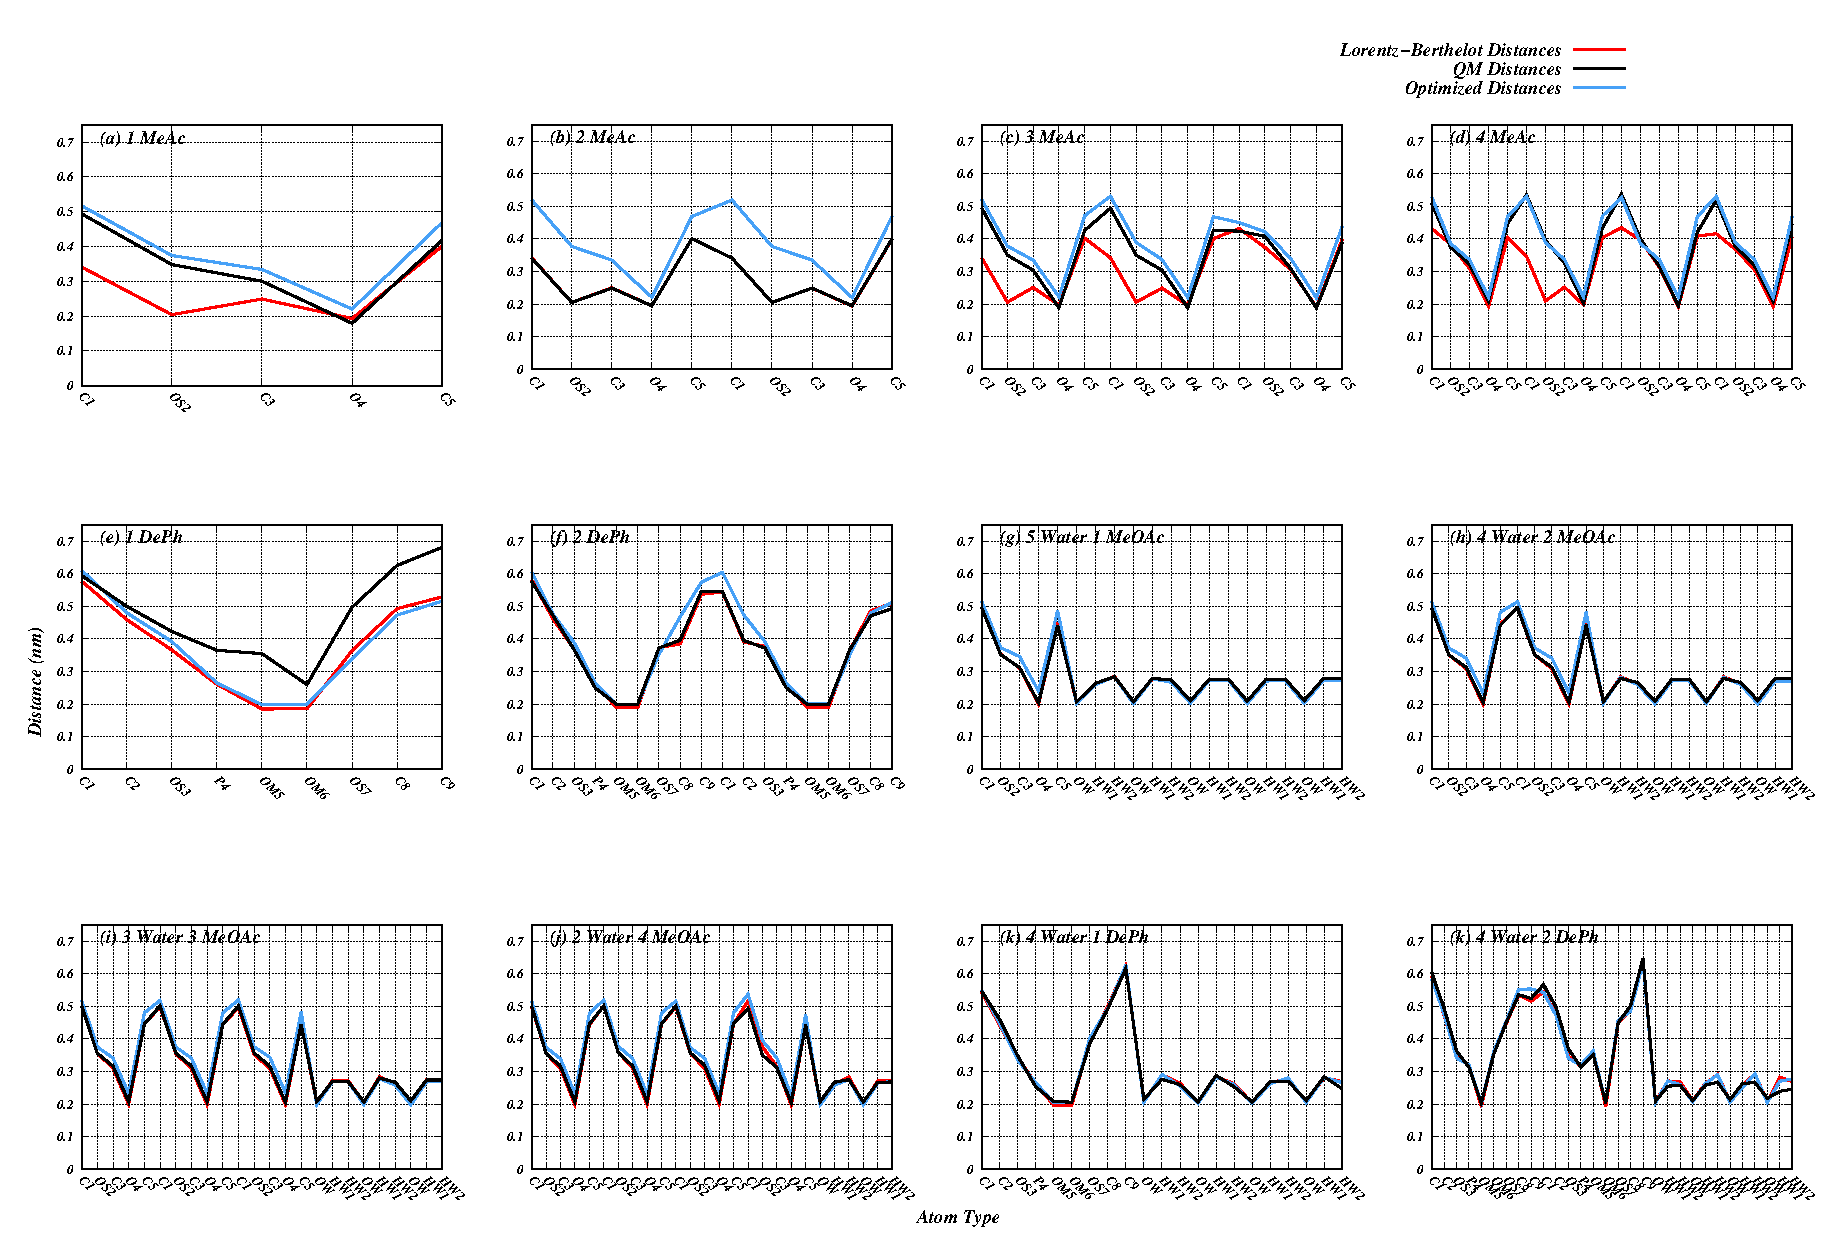
\includegraphics[height=\textheight]{Figure_S1.eps}
\end{figure}
\end{landscape}
We note substantial improvements in both substitution energies with a minimal loss of accuracy in geometries, 
with parameter optimization reducing mean absolute error in $\Delta E_{sub}$ from 0.26 to 0.01. %, and reducing mean absolute error in distances of Mg from cluster atoms from XX to YY \AA.

\begin{table}[h!]
\centering
\begin{tabularx}{\textwidth}{|X|X|X|X|X|X|X|}
\hline
                         & \multicolumn{2}{c|}{\textbf{2025}} & \multicolumn{2}{c|}{\textbf{2024}} & \multicolumn{2}{c|}{\textbf{LB-rules}} \\\hline
Parameter                & \boldmath$\varepsilon$             & \boldmath$\sigma$                  & \boldmath$\varepsilon$                          & \boldmath$\sigma$ & \boldmath$\varepsilon$ & \boldmath$\sigma$ \\\hline
MG-CH3                   & 0.60498                            & 0.22161                            & 0.68709                                         & 0.14257           & 0.19239                & 0.30856 \\\hline
MG-CH2                   & 1.36553                            & 0.41404                            & 0.63126                                         & 0.20617           & 0.13238                & 0.32468 \\\hline
MG-OA                    & 25.25725                           & 0.30372                            & 5.05190                                         & 0.26223           & 0.19044                & 0.26890 \\\hline
MG-P                     & 29.74732                           & 0.23348                            & 3.89200                                         & 0.27811           & 0.32318                & 0.29044 \\\hline
MG-OM\textsuperscript{*} & 22.04699                           & 0.20018                            & 3.22262                                         & 0.17691           & 0.20771                & 0.26469 \\\hline
MG-CO\textsuperscript{*} & 0.57040                            & 0.42212                            & 0.56152                                         & 0.37127           & 0.06152                & 0.34796 \\\hline
MG-O\textsuperscript{*}  & 2.06827                            & 0.24468                            & 2.43058                                         & 0.13069           & 0.20771                & 0.26469 \\\hline
\end{tabularx}
\caption[Lennard-Jones cross-terms]{Lennard-Jones parameters for magnesium interactions: well depth $\epsilon_{ij}$ (kJ/mol) and distance parameter $\sigma_{ij}$ (nm), comparing the 2025 optimized model, the 2024 model, and the original LB-rules.}
\label{tabch4:params}
\end{table}

% \begin{table}[h!]
% \centering
% \begin{tabular}{lcccc}
% \hline
%  & $n$ & QM & LB rule & Optimized \\
% \hline
% MeAc  & 1 & -71.29   &    -59.18& -71.28  \\\hline
%     & 2 & -127.20  &   -112.47& -122.88 \\\hline
%     & 3 & -166.16  &   -155.99& -167.84 \\\hline
%     & 4 & -192.53  &   -187.59& -192.28 \\\hline
% DEPh & 1 & -775.55  &   -312.57& -754.82 \\\hline
%     & 2 & -1333.69 &   -553.24& -1333.65 \\\hline
% \hline
%          & MAPE & &0.26 &0.01 \\
% \hline
% \end{tabular}
% \caption[Substitution energies]{Energies (kJ/mol) associated with substituting $n$ water molecules in 6-fold Mg-water clusters with $n$ methyl acetates (MeAcs) or $n$ diethyl phosphates (DEPhs). Substitution energies are defined in equation \ref{equ_2}.}
% \label{tabch4:subenergies}
% \end{table}

% Combined comparison: LB Rules vs 2024 vs 2025
\begin{landscape}
\begin{table}[htbp]
\centering
\sisetup{round-mode=places,round-precision=3,detect-all}
\begin{tabular}{
  l
  S[table-format=-7.3] % PBE0+VdW
  S[table-format=-7.3] S[table-format=1.3] S[table-format=1.3] % LB Rules
  S[table-format=-7.3] S[table-format=1.3] S[table-format=1.3] % 2024
  S[table-format=-7.3] S[table-format=1.3] S[table-format=1.3] % 2025
}
\toprule
& {PBE0+VdW} 
& \multicolumn{3}{c}{LB Rules} 
& \multicolumn{3}{c}{2024} 
& \multicolumn{3}{c}{2025} \\
\cmidrule(lr){2-2}\cmidrule(lr){3-5}\cmidrule(lr){6-8}\cmidrule(lr){9-11}
{System} & {Ref.}
& {Energy} & {Abs.\%} & {MAPE}
& {Energy} & {Abs.\%} & {MAPE}
& {Energy} & {Abs.\%} & {MAPE} \\
\midrule
1MeOAc    & -268.702 & -130.319 & 0.515 & {}
                    & -299.844 & 0.116 & {}
                    & -32.724  & 0.878 & {} \\
2MeOAc    & -449.770 & -243.856 & 0.458 & {}
                    & -545.386 & 0.213 & {}
                    & -59.544  & 0.868 & {} \\
3MeOAc    & -550.360 & -263.968 & 0.520 & {}
                    & -598.606 & 0.088 & {}
                    & -42.191  & 0.923 & {} \\
4MeOAc    & -609.631 & -341.534 & 0.440 & 0.483
                    & -690.483 & 0.133 & 0.137
                    & -98.578  & 0.838 & 0.877 \\
1DEPh     & -942.545 & -972.812 & 0.032 & {}
                    & -1063.300& 0.128 & {}
                    & -772.729 & 0.180 & {} \\
2DEPh     & -1302.053& -1051.842& 0.192 & 0.112
                    & -1488.761& 0.143 & 0.136
                    & -1248.054& 0.041 & 0.111 \\
5W 1MeOAc & -71.288  & -91.759  & 0.287 & {}
                    & -165.829 & 1.326 & {}
                    & -71.280  & 0.000 & {} \\
4W 2MeOAc & -127.201 & -177.528 & 0.396 & {}
                    & -316.012 & 1.484 & {}
                    & -122.881 & 0.034 & {} \\
3W 3MeOAc & -166.160 & -253.576 & 0.526 & {}
                    & -402.648 & 1.423 & {}
                    & -167.835 & 0.010 & {} \\
2W 4MeOAc & -192.534 & -317.715 & 0.650 & 0.465
                    & -507.049 & 1.634 & 1.467
                    & -192.275 & 0.001 & 0.011 \\
4W 1DEPh  & -775.546 & -640.060 & 0.175 & {}
                    & -848.090 & 0.094 & {}
                    & -754.821 & 0.027 & {} \\
4W 2DEPh  & -1279.754& -1198.284& 0.064 & 0.119
                    & -1519.772& 0.188 & 0.141
                    & -1333.653& 0.042 & 0.034 \\
\bottomrule
\end{tabular}
  \caption{Energies (kJ/mol) associated with substituting $n$ water molecules in low coordination clusters, and in 6-fold Mg-water clusters with $n$ methyl acetates (MeAcs) or $n$ diethyl phosphates (DEPhs). 
  Substitution energies are defined in equation \ref{equ_2}.}
  \label{tabch4:subenergies}
\end{table}
% \begin{table}[h!tbp]
% \centering
% \sisetup{round-mode=places,round-precision=3,detect-all}
% \begin{tabular}{l S[table-format=+4.3]}
% \toprule
% {Cluster} & {$\Delta(\Delta E_{\text{sub}})$ (2025--2024)} \\
% \midrule
% % --- MeOAc ---
% 1MeOAc     & +267.120 \\
% 2MeOAc     & +485.842 \\
% 3MeOAc     & +556.415 \\
% 4MeOAc     & +591.905 \\
% 5W\,1MeOAc & +94.549  \\
% 4W\,2MeOAc & +193.131 \\
% 3W\,3MeOAc & +234.813 \\
% 2W\,4MeOAc & +314.774 \\
% \midrule
% % --- DEPh ---
% 1DEPh      & +290.571 \\
% 2DEPh      & +240.707 \\
% 4W\,1DEPh  & +93.269  \\
% 4W\,2DEPh  & +186.119 \\
% \bottomrule
% \end{tabular}
% \caption{Differences in substitution energies 
% $\Delta(\Delta E_{\text{sub}}) = 
% \Delta E_{\text{sub}}^{2025} - \Delta E_{\text{sub}}^{2024}$ 
% for MeOAc and DEPh clusters, including mixed six-fold water–ligand clusters.}
% \label{tab:delta-sub-combined}
% \end{table}
\begin{table}[htbp]
\centering
\sisetup{round-mode=places,round-precision=3,detect-all}
\begin{tabular}{
  l
  S[table-format=+6.3]
  S[table-format=+6.3]
  S[table-format=+6.3]
}
\toprule
{Cluster} &
{$\Delta E_{\text{sub}}^{2024}-\Delta E_{\text{sub}}^{\text{LB}}$} &
{$\Delta E_{\text{sub}}^{2025}-\Delta E_{\text{sub}}^{\text{LB}}$} &
{$[2025{-}2024]$} \\
\midrule
% --- MeOAc (no waters) ---
1MeOAc     & -169.525 & +97.595 & +267.120 \\
2MeOAc     & -301.531 & +184.311 & +485.842 \\
3MeOAc     & -334.638 & +221.777 & +556.414 \\
4MeOAc     & -348.949 & +242.956 & +591.905 \\
% --- MeOAc mixed 6-fold ---
5W\,1MeOAc &  -74.071 &  +20.479 &  +94.550 \\
4W\,2MeOAc & -138.484 &  +54.647 & +193.131 \\
3W\,3MeOAc & -149.072 &  +85.741 & +234.813 \\
2W\,4MeOAc & -189.334 & +125.440 & +314.774 \\
\midrule
% --- DEPh (no waters) ---
1DEPh      &  -90.488 & +200.083 & +290.571 \\
2DEPh      & -436.919 & -196.211 & +240.708 \\
% --- DEPh mixed 6-fold ---
4W\,1DEPh  & -208.031 & -114.761 &  +93.270 \\
4W\,2DEPh  & -321.488 & -135.369 & +186.119 \\
\bottomrule
\end{tabular}
\caption{Shifts in substitution energies relative to LB Rules:
$\Delta E_{\text{sub}}^{202X}-\Delta E_{\text{sub}}^{\text{LB}}$ for 2024 and 2025,
and their difference $[2025{-}2024]$.
Positive values mean 202X is less stabilizing (less negative) than LB; negative values
mean more stabilizing than LB.}
\label{tab:subs-relative-to-lb}
\end{table}
\end{landscape}

\subsection{Bilayer Construction}

Simulation systems are prepared following the general procedure in
Chapter~1~\cite{saunders:2024}. Each system contains 200 POPC lipids
(100 per leaflet) and 60,000 waters. To achieve a starting concentration
of 200~mM \mgcl, 216 waters are replaced with \mg{} and 432 with \cl{}.
These configurations are used for both the \mg{2025} HFE and micro
simulations.

\subsection{Molecular Dynamics}

Two 1~$\mu$s production simulations are performed using the \mg{2025}
parameters: one with the water--\mg{} interaction term from the HFE
model of Li \etal~\cite{merzhfe}, and one with the \mg{} micro model of
Grotz \etal~\cite{grotz:2021:optimized,micro}. Lipid interactions are
described with the gromos43A1-S3 force field~\cite{chiu:2009}.
Trajectory analysis is carried out with GROMACS built--in tools,
in--house code using the GROMACS API, and the MDAnalysis Python
package~\cite{mdanalysis1,mdanalysis2}.

\section{Results and Discussion}

\subsection{Water structure, and hydration boundaries}
To differentiate interfacial ions from those in the bulk solvent, we first need to define at interfacial boundary. As before\cite{saunders:2024}, we do this using the orientational ordering of water molecules. Waters near the lipid bilayer interface are ordered due to the electrostatic and steric interactions with the lipid bilayer, as well as interactions with dissolved salts. The
orientation of these waters can be probed by computing the orientational order parameters $P_1=\langle\cos{\beta}\rangle$ and $P_2=\langle{\frac{1}{2}(3\cos^{2}{\beta}-1}\rangle$, where $\beta$ is the angle made between the water OW-HW1 vector and the box z-axis. The hydration boundary marks the location where water molecules become orientationally isotropic, beyond which they no longer contribute to quadrupolar NMR splitting. We use this boundary to distinguish between adsorbed ions and ions in bulk solvent. In our previous work~\cite{saunders:2024}, we demonstrated that ion densities outside this boundary follow Poisson–Boltzmann theory, while those inside deviate from it. This breakdown in mean-field behavior indicates a specific interaction with the membrane. 

To compute $P_1$ and $P_2$, we divide the simulation unit cell into 2000 slices along the membrane transverse (z-) axis.  
The average values over the last 150 ns of the simulation are plotted in figure~\ref{figch4:h2order}, with points shown for every 200 slices. 

\begin{figure}[H]
    \caption[Water orientational order parameters]{Water orientation order parameters. The first
    order parameter represents an in-out ordering with respect to the bilayer center, and the second is related to the orientation of the quadrupole moment of the box. A value of zero is completely
    parallel with the box axis.  
    The first order parameter indicates a significant increase in the positive ordering induced by the \mg{ 2025} parameters compared to the no-salt and the
        \mg{ 2024} simulations.  The second order parameter indicates increased ordering as on approaches the bilayer starting from the boundary with bulk solvent, indicated by the set of dotted lines
        furthest from the bilayer center point. Ordering increases as we approach the bilayer \dhh{}, indicated by the second set of dotted lines. There is also a steeper decline as one follows the plot into to the acyl chain region denoted by the bilayer \dc{} -- denoted by the innermost dotted lines --  in the
\mg{ 2025} Micro system. We note that the hydration boundary of both of the 2025 simulations is further from the bilayer center compared to the 2024 simulations, resulting in a larger region of biological water
at the bilayer surface. This alone can result in a greater number of ions adsorbed in at least the \emph{steric} adsorption mode.} 
    \label{figch4:h2order}
    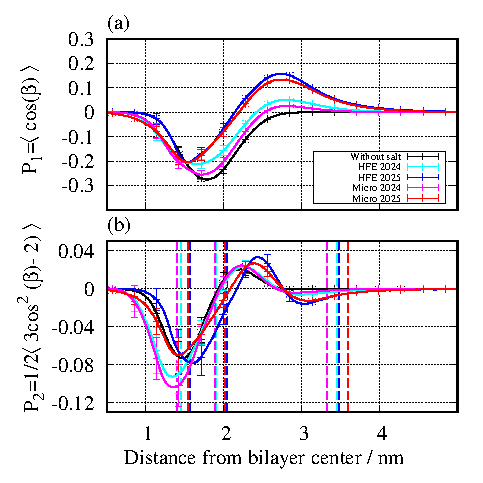
\includegraphics{Figure_1.eps}
\end{figure}
The histogram of $P_2$ is used to calculate the \emph{hydration boundary} of the lipid bilayer system. The outermost
region of negative ordering is fitted to an exponential function, and the length scale of the exponential is used to find the location where $P_2$ is considered to be effectively zero. 
Lines to delimit these values are drawn on the plot in figure~\ref{figch4:h2order}, and these positions are noted for each bilayer
in table~\ref{tabch4:struc}.
\begin{table}
{\tiny
    \caption[Bilayer structural parameters]{Bilayer structural parameters. The bilayer hydration boundary is defined as the position away from the bilayer center beyond which solvent is isotropic, and denotes 
        bulk solvent from bound solvent. The number of adsorbed charges in each adsorption mode are within the hydration boundary of the system, and are further classified by the degree
    of loss of hydration water -- steric adsorbed have lost no water, imperfect have lost at least one, and perfect have replaced all water oxygens for lipid oxygens. The bilayer thickness
\dhh{} is defined as the distance between the peaks in the electron density of the system, roughly localizing the phosphate groups. \dc{} is the thickness of the acyl-chain region of the bilayer,
and is measured as the distance between the Gibb's surfaces of the acyl-chain probability density. Lipid component volumes $V_{CH3}$ and $V_{\text{CH1/CH2}}$ are computed using the method
of Petrache \etal{}~\cite{petrache:1997}. $V_C$ is computed from the component volumes by multiplying by the number of these components in each acyl chain. 
$A_L=\frac{V_C}{D_C}$ is the two-dimensional area occupied per lipid on the bilayer surface. We note a correlation between simulations with larger numbers of adsorbed charges
and perturbation of the bilayer structure from that of the simulation without salt, especially in the bilayer \dc{}.}
    \label{tabch4:struc}
    \begin{tabularx}{\textwidth}{|X|X|X|X|X|X|}

        \hline                     & Without salt             &  \mg{ 2024} HFE     & \mg{ 2024} Micro    & \mg{ 2025} HFE    & \mg{ 2025} Micro \\\hline
    Hydration Boundary~(\AA)       & N/A                      &  34.5               & 33.3               & 34.8               & 35.9      \\\hline
    Perfectly Adsorbed Charges     & 0                        &  1.90               & 0.00               & 0.00               & 0.00      \\\hline
    Imperfectly Adsorbed Charges   & 0                        &  3.68               & 6.23               & 28.43              & 96.93     \\\hline
    Sterically Adsorbed Charges    & 0                        &  37.11              & 31.45              & 106.00             & 20.11     \\\hline
    $D_{HH}$~(\AA)                 & 37.57 $\pm$ 1.27         &  38.15 $\pm$ 1.20   & 37.75 $\pm$ 1.19   & 40.75 $\pm$ 0.92   & 40.26 $\pm$ 0.96\\\hline
%    $D_b$~(\AA)                    & 36.25 $\pm$ 0.47        & 43.01 $\pm$ 0.49   & 41.81 $\pm$ 0.52   & 46.24 $\pm$ 0.39   & 45.75 $\pm$ 0.42\\\hline
    $2D_C$~(\AA)                   & 26.98 $\pm$ 0.35         &  28.99 $\pm$ 0.31   & 28.08 $\pm$ 0.40   & 31.45 $\pm$ 0.29   & 30.84 $\pm$ 0.29\\\hline
    $V_{\text{CH1/CH2}}$~(\AA$^3$) & 26.33 $\pm$ 0.05         &  26.21 $\pm$ 0.05   & 26.33 $\pm$ 0.05   & 26.22 $\pm$ 0.04   & 26.12 $\pm$ 0.04\\\hline
    $V_{CH3}$~(\AA$^3$)            & 54.97 $\pm$ 0.39         &  54.77 $\pm$ 0.39   & 54.98 $\pm$ 0.40   & 54.74 $\pm$ 0.24   & 55.19 $\pm$ 0.26\\\hline
%    $V_H$~(\AA$^3$)                & 323.30 $\pm$ 0.82       & 323.95 $\pm$ 1.26  & 327.85 $\pm$ 1.10  & 283.55 $\pm$ 0.77  & 296.16 $\pm$ 0.67\\\hline
    $V_C$~(\AA$^3$)                & 899.72 $\pm$ 1.01        &  895.85 $\pm$ 1.05  & 899.83 $\pm$ 1.06  & 895.94 $\pm$ 0.95  & 894.00 $\pm$ 1.11\\\hline
%    $V_L$~(\AA$^3$)                & 1223.01 $\pm$ 0.82      & 1219.80 $\pm$ 1.24 & 1227.68 $\pm$ 1.24 & 1179.49 $\pm$ 1.02 & 1190.16 $\pm$ 1.07\\\hline
    $A_L=\frac{V_C}{D_C}$          & 66.71 $\pm$ 0.89         &  61.80 $\pm$ 0.66   & 64.10 $\pm$ 0.92   & 56.97 $\pm$ 0.54   & 57.98 $\pm$ 0.57\\\hline
    \end{tabularx}
}
\end{table}
\section{\mg Adsorption Behavior}
We classify any ion within the hydration boundary as at least sterically adsorbed, with further distinction -- steric, imperfect, or perfect -- based on how much dehydration the ion undergoes when approaching the bilayer center. A \emph{perfectly} adsorbed ion has lost all waters in its first hydration shell and an  \emph{imperfectly} adsorbed ion
has lost at least one water from its first coordination shell. 
{\emph{Sterically} adsorbed} waters have their first shell of waters intact, but 
they are spatially located within the \emph{hydration boundary} of the lipid bilayer. To evaluate this, we define a cutoff to the first hydration shell,
computed from radial distribution functions. The cutoff used for \mg{} in all systems is 3.3~\AA, which captures the first peak for \mg{} and lipid oxygens, water, and \cl{}. 
We compute the nearest oxygens (lipid phosphate, glycerol, ester fragment, \cl{}, or water) within these
cutoffs of cations across the simulation system, and generate a histogram averaged over slices and then over the last 150 ns of simulation time. This histogram is shown in 
figure~\ref{figch4:ioncoordination}.
\begin{figure}[H]
    \caption[First-shell coordination partners of \mg]{Coordination partners of \mg{}. We note that while the Micro water with the 2024 parameters do result in some dehydration 
        of the \mg{} in the headgroup region of the bilayer, both 2024 parameters yield nearly no dehydration of \mg{} at any location in the simulation box. The 2025 HFE parameters
        still largely do not dehydrate, but the 2025 Micro parameters do result in loss of 1-2 waters from the \mg{} coordination shell within the headgroup region. 
        We see substantial interaction with the headgroup phosphate oxygens, and no significant interaction with the glycerol or ester linkage oxygens. We also note the increased interaction with \cl{} in the 
    simulations using the 2025 parameters compared to both simulations with the 2024 parameters. The number of first shell \cl{} remains below one per ion in any simulation.}
\label{figch4:ioncoordination}
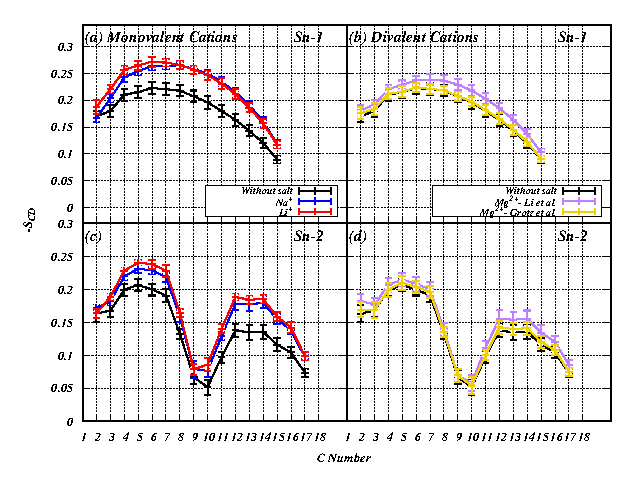
\includegraphics[height=0.5\textheight]{Figure_2.eps}
\end{figure}
We note that the \mg{ 2024} parameters result in very little dehydration of ions, throughout the simulation box. The 2025 parameters result in loss of 1-2 waters as the ion approaches the bilayer center, with the \mg{ 2025} Micro parameters resulting in the greatest degree of dehydration among parameter sets.
The \mg{ 2025} HFE parameters result in some loss of first shell water, but no replacement in the first shell with lipid oxygens. There are a significant number of \mg{}-\cl{} pairs, where a single \cl{} replaces a water
in the first shell of \mg{} as the ion moves into the lipid-occupied region of the bilayer. If these ions do not otherwise lose water for lipid parts, 
they are counted as \emph{sterically} adsorbed.

The \mg{ 2025} Micro parameters appear to have a preference for direct interaction with the phosphate group oxygens when dehydrated, and none of the \mg{} parameters studied result in significant direct interaction with the ester fragment and glycerol oxygens. There are also far fewer pairs with \cl{} under this parameter set.
Fractions of ions in each adsorption mode have been computed by counting the number of ions in each frame within the hydration boundary, 
and the number of those that have lost one water, or all of their waters. We compute averages over the last 150ns, and then 
fractions of the total adsorbed ions present in each mode. These values are shown in figure~\ref{figch4:adfrac}, alongside the fraction of ions adsorbed vs the fraction remaining in bulk solvent. 
\begin{figure}[H]
    \caption[Fraction of ions in each adsorption modality]{ (a) Distribution of \mg{} ions in different membrane adsorption modes. \mg{} are first classified into those in bulk and those adsorbed in membranes. 
        Among those adsorbed in membrane, \mg{} are 
        further classified into those that are perfectly, imperfectly and sterically adsorbed. 
        We note that compared to the 2024 models, the 2025 models result in increased membrane adsorption, 
        and among the adsorbed \mg{}, the 2025 models result in increased direct coordination with lipid headgroups. Next to the plot, we show examples of \mg{} in the \emph{steric} (b) and \emph{imperfect} (c) 
        adsorption modes from our simulations. The \emph{perfect} adsorption mode does not occur in a significant frequency in \mg{}, so an example is not included. We note that
    in this example of the \emph{steric} adsorption mode (b) there is a \cl{} (green) included in the hydration shell of the \mg{} ion (magenta). This is an example of a partial-ion
pair, which while having lost a water from the first-shell, it is not coordinating lipid components directly -- these are counted as sterically adsorbed.}
    \label{figch4:adfrac}
    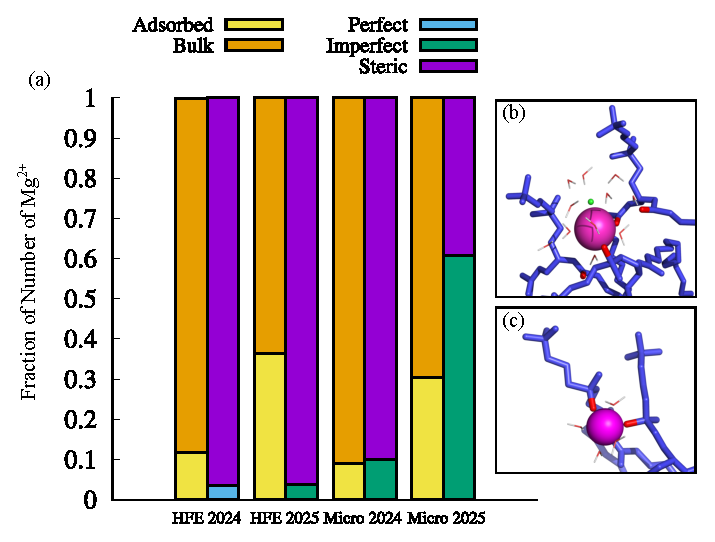
\includegraphics[height=0.5\textheight]{Figure_3.eps}
\end{figure}
The 2025 parameters result in significantly more adsorbed ions and as a result more adsorbed charges in both cases, with the most increased in the \mg{ 2025} HFE simulation.
We count the number of adsorbed charges in each adsorption mode by multiplying the number of ions in each mode by their charge; this would be 2 charges per \mg{}, and a \mg{} paired with a \cl{}
counts a single charge. 
These numbers can be seen in table~\ref{tabch4:struc} rows 2-4.
We also note an increase in imperfectly adsorbed ions in the \mg{ 2025} HFE simulation. However, the \mg{ 2025} Micro parameters result in ions shifting to the majority in the imperfect
adsorption mode from the steric mode seen in both 2024 simulations.
The \mg{ 2025} HFE parameters still remain with the largest fraction of ions in the steric adsorption mode. 
These differences in the distribution of adsorbed \mg{} ions -- particularly the rise in imperfect adsorption for \mg{ 2025} Micro -- 
raises the question of how such interactions reshape the membrane itself. We therefore turn to a structural analysis of the lipid bilayer 
to evaluate the consequences of these adsorption patterns.


\section{Bilayer Structure}
The effect of changes in ion adsorption on bilayer structure was assessed through several structural parameters. Electron densities were
computed using the \texttt{gmx density} tool included in the GROMACS software suite. Histograms were calculated in 1 ns chunks along the
bilayer normal (z-axis) and centered at zero using the position of minimum density, corresponding approximately to the bilayer midplane.
These histograms were then symmetrized about the center and averaged over the final 150 ns of each trajectory.

From the resulting profiles, we calculated the small-angle X-ray scattering (SAXS) form factor by subtracting the average water electron
density and applying a cosine transform. Electron density profiles and corresponding simulated SAXS form factors are shown in
Figure~\ref{figch4:formfactors}.

\begin{figure}[H]
    \caption[SAXS formfactors]{SAXS form-factors and associated electron densities for \mg{} simulations. (a) \mg{ 2024} under both Micro
and HFE has little effect in changing the bilayer form-factor compared to that of the no-salt simulation, consistent with the available experimental results at lower ion concentrations. 
Conversely, both of the simulations with 2025 parameters result in significant thickening of the bilayer. 
This is also seen in the associated electron densities (b), where we see much taller peaks that are further apart in the \mg{ 2025} simulations
than that obtained from the 2024 simulations.}
    \label{figch4:formfactors}
    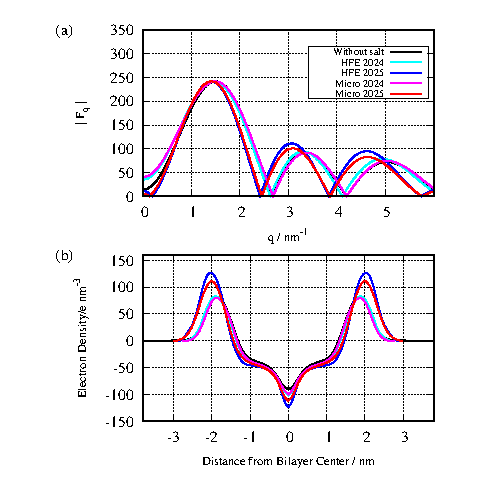
\includegraphics[height=0.5\textheight]{Figure_4.eps}
\end{figure}
We note significant broadening of the bilayer peak-to-peak distance in the electron densities of the 2025 systems, compared to the 2024 systems. 
Additional structural parameters are computed from the various number density histograms of our simulations. Similarly to the electron densities, we use the gromacs GMX density tool to compute the number density histogram over 1ns chunks of our simulation. We then center these histograms using the centerpoint found from the electron
density at each 1ns chunk. 
These histograms are then symmetrized, and averaged over the last 150ns of simulation time. 
These can be seen for solvent and lipid headgroup components of in figure~\ref{figch4:soldens}.
We note greater accumulation of \mg{} in the \mg{ 2025} simulations, with greater peak densities of cations in the headgroup regions, with the largest peak in the \mg{ 2025} HFE system. 

\begin{figure}[H]
    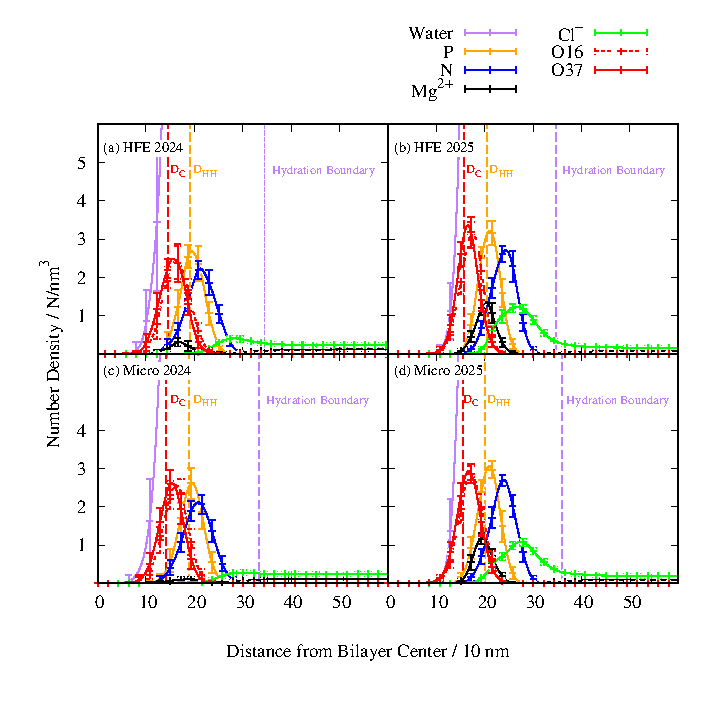
\includegraphics{Figure_5.eps}
    \caption[Number densities]{Number density histograms of lipid headgroup components. Vertical lines denote the bilayer structural features such as the hydration boundary in purple, the \dhh{} in orange and the \dc{} in red. We note
    that within the hydration boundary of each system there is accumulation of ions -- anions accumulate near the trimethylammonium nitrogen and cations accumulate near the phosphate group. The \mg{ 2025} parameters
have a much larger accumulation of both ions in the headgroup region of the bilayer compared to the \mg{ 2024} systems.}
    \label{figch4:soldens}
\end{figure}

The bilayer thickness \db{} and the acyl-chain region thickness \dc{} are computed as the distance between the Gibb's surfaces of the probability densities of solvent and the lipid acyl-chain carbons, respectively~\cite{fogarty:2015}. 
These are computed from the number densities of these species for each 1ns chunk of the simulation, and then averaged over the last 150ns of the simulation time.
The values for these are listed in table~\ref{tabch4:struc}. 
We also compute the lipid component volumes using the method of Petrache \etal{}~\cite{petrache:1997}. To do this, we partition the lipid number densities into 
headgroup and chains, with the headgroup consisting of any particles above the acyl chain ester fragment and the chains as just the acyl chain carbons. We partition the
chains into groups of CH2+CH1, and the terminal CH3 atoms. We optimize the following objective function to partition the volume in each histogram slice $z_j$ from the number densities to these groups:
\begin{equation}
    \Omega{(v_i)}=\sum^{\rho_s}_{z_j}\bigg(1-\sum^{N_{\text{groups}}}_{i=1}\big(\rho_i(z_j)(v_i)^2\bigg)\text{.}
\end{equation}
From this we obtain partial volumes for the groups $v_{\text{CH1\&CH2}}$, $v_{\text{CH3}}$, $v_{\text{Headgroup}}$. We equate the $V_{CH2}=v_{CH1\&CH2}$ as these densities have significant overlap, 
and thus the volumes cannot be separated. This, along with the $V_{\text{CH3}}=v_{\text{CH3}}$ can be seen in table~\ref{tabch4:struc}. These volumes multiplied by the number of each 
moiety in a lipid are used to compute \Vc. Finally, we compute the \al as the ratio $2\times{}V_c/2D_C$.

\subsection{Acyl-Chain order parameters}
Acyl-chain order parameters are computed using the method outlined by Douliez \etal~\cite{Douliez:1995} (see  figure~\label{fig:acylorder}). We note that
the 2024 \mg{} parameters do not significantly increase the acyl-chain ordering from that of the system simulated without salt.The 2025 \mg{} parameters have a much greater effect on the ordering.
\begin{figure}[h!]
   \caption[Acyl-Chain order parameters]{Acyl-chain CD Order parameters. We note increased ordering in the
   simulations using the 2025 model parameters, while the 2024 parameters result in
bilayers that remain very similar to the simulation without salt.}
   \label{fig:acylorder}
   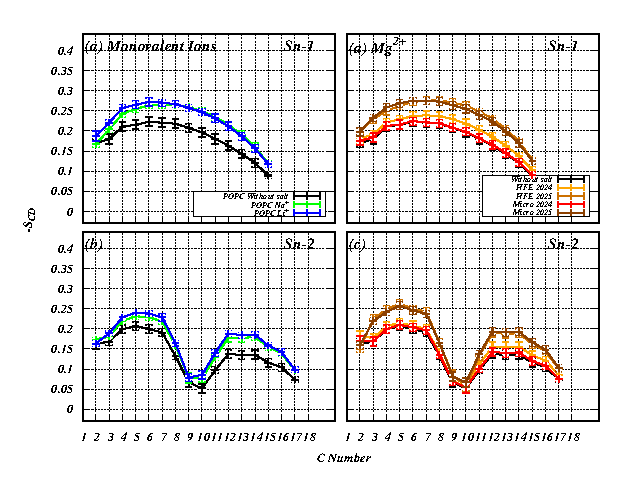
\includegraphics{op.eps}
\end{figure}
We can compute the lipid bilayer thickness using the acyl-chain order parameter by using the
"first-order mean-torque model" of Petrache \etal~\cite{petrache:2000:nmrarea,nagle:2000}.
This is done by taking the average S\textsubscript{CD} from the experimental plateau region -- the set of carbons where the experimental S\textsubscript{CD} does not change
detectably~\cite{nagle:2000,nagle:1993:nmrarea}. This can be used to compute the average segmental projection onto the bilayer normal $\langle x \rangle$:
\begin{equation}
   \langle x \rangle = 1 - \frac{1}{\varepsilon_1}, \varepsilon_1 = \frac{2}{1 - \sqrt{\frac{-8\big<S_{CD}\big> - 1}{3}}}\text{,}
\end{equation}
where $\varepsilon_1$ is the mean-torque parameter. We compute the corresponding squared projection $\langle x^2 \rangle$ from the $S_{CD}$
using the following equation:
\begin{equation}
   \langle x^2 \rangle = \frac{1 - 4\big<S_{CD}\big>}{3}\text{,}
\end{equation}
which can be used together to compute the area factor:
\begin{equation}
q = 3 - 3 \langle x \rangle + \langle x^2 \rangle\text{.}
\end{equation}
This is then used to compute both the area per lipid and the thickness of the acyl-chain region of the lipid bilayer:
\begin{equation}
   \langle A \rangle = q\frac{4V_{\text{CH}_2}}{D_M}\text{,}
\end{equation}
Using $V_{CH_2}$ computed from the number densities, and the bond length $D_M=2.54$.
We approximate the $V_{CH2}$ in two ways from the $v_{CH2\&CH1}$ -- first by directly using $V_{CH2}=v_{CH2\&CH1}$, and
second by using the common approximation of $\frac{V_{CH2}=v_{CH3}}{2}$~\cite{nagle:2000}.
These values are listed in table \ref{tab:opstruc}. We can also compute the acyl chain thickness:
\begin{equation}
   D_C = \frac{n_cD_M}{2q}\text{,}
\end{equation}
with $n_c=16$ as the number of carbons in the Sn-1 chain.
These values can be seen in table~\ref{tab:opstruc}.
%This is considered to be a more reliable measure of the lipid bilayer thickness than the other measures such as the peak-to-peak
%distance from the electron densities \dhh{} or
%the Gibbs-Luzzati thickness \db{},
%where both the water structure and the headgroup tilt have significant influence over the result~\cite{nagle:2000}. Also, computing the \dc{} in this way
%is independent of the number densities as the $V_{CH2}$ is computed using densities, as well as the acyl-chain probability density used for
%the gap--integral. \TODO I DONT CARE FOR THIS PART!!! WHY LEAVE TODOS????
\begin{table}
{\tiny
   \caption[\dc{} and \al{} from acyl chain ordering]{Area factor, acyl chain region thickness and area per lipid. These values are computed via the method described in Petrache \etal~\cite{petrache:2000:nmrarea}. This provides us with another
   measure of the acyl chain thickness. We note that the thickening of the lipid bilayer remains consistent with the acyl chain thickness \dc{} computed from the number densities.}
   \label{tab:opstruc}
   \begin{tabularx}{\textwidth}{X|X|X|X|X|X|X|X}
   \multicolumn{4}{l}{ }                       & \multicolumn{2}{l}{2024} & \multicolumn{2}{l}{2025}\\\hline
                                               & Without salt             & \na                              & \li                & \mg-HFE            & \mg-Micro          & \mg-HFE            & \mg-Micro \\\hline
   $q$                                         & 1.39 $\pm$ 0.14          & 1.30 $\pm$ 0.11                  & 1.29 $\pm$ 0.02    & 1.36 $\pm$ 0.02    & 1.41 $\pm$ 0.03    & 1.24 $\pm$ 0.01    & 1.26 $\pm$ 0.01 \\\hline
   $2D_C$ NMR~(\AA)                            & 28.67 $\pm$ 2.97         & 30.85 $\pm$ 2.57                 & 31.53 $\pm$ 0.53   & 29.98 $\pm$ 0.47   & 28.84 $\pm$ 0.57   & 32.66 $\pm$ 0.33   & 32.17 $\pm$ 0.30\\\hline
   $A_L$ from $v_{CH2\&CH1}$                   & 55.14 $\pm$ 1.21         & 51.98 $\pm$ 0.69                 & 53.13 $\pm$ 0.91   & 55.98 $\pm$ 0.92   & 58.45 $\pm$ 1.16   & 51.37 $\pm$ 0.52   & 51.97 $\pm$ 0.49 \\\hline
   $((V_{CH3}/2)$                              & 30.87 $\pm$ 0.30         & 29.65 $\pm$ 0.24                 & 27.58 $\pm$ 0.19   & 27.40 $\pm$ 0.19   & 27.49 $\pm$ 0.20   & 27.38 $\pm$ 0.13   & 27.59 $\pm$ 0.13 \\\hline
   $A_L$ from  $(V_{CH3}/2)$                   & 68.26 $\pm$ 1.95         & 61.10 $\pm$ 0.99                 & 56.02 $\pm$ 1.04   & 58.51 $\pm$ 1.03   & 61.03 $\pm$ 1.35   & 53.67 $\pm$ 0.58   & 54.90 $\pm$ 0.60 \\\hline
   \end{tabularx}
}
\end{table}
Notably, the \dc{} for all systems studied is slightly smaller than what we compute from the number densities, but follows similar trends.
The \al{} computed here only relies on the volume of the CH2 moiety, and ends up with again
quite different results than what we computed from $2V_C/2D_C$.

We note that in the systems with the smallest number of adsorbed charges in non-steric modes (perfect and imperfect) -- in this case the 2024-\mg parameters, show 
the smallest increase in \dc{}. The \mg{ 2025} systems have the greatest number of adsorbed charges in non-steric modes, 
and have the largest increase in \dc{} over the system simulated without salt. We note that
this trend is not followed necessarily in the \dhh{}, which is not a reliable measures of bilayer thickness due to the effect of headgroup tilt angle, and overlapping number densities of water
and salt in the headgroup region.
Together, we note that the systems with the greatest number of charges in the Langmuir-type (non-steric) modes correlate with an increase the 
bilayer thickness (figure~\ref{figch4:chargeperlipid})
\begin{figure}[h!]
    \caption[Adsorbed charge per adsorption modality]{Adsorbed charge per adsorption modality per lipid as a function of the lipid bilayer hydrocarbon thickness \dc{}. We compare both our results from this work, and our previous work with monovalent
        ions~\cite{saunders:2024}. There is a clear trend in the total number of adsorbed
        charges (i.e. any charges not in bulk solvent), where more charges results in a greater \dc{}. However, if one examines the sterically adsorbed charges, the trend is not as strong. This seems to indicate
    that the non-steric charges are most responsible for the pertubation of the bilayer thickness from that of the no-salt simulation shown as the blue region on the plot.}
    \label{figch4:chargeperlipid}
    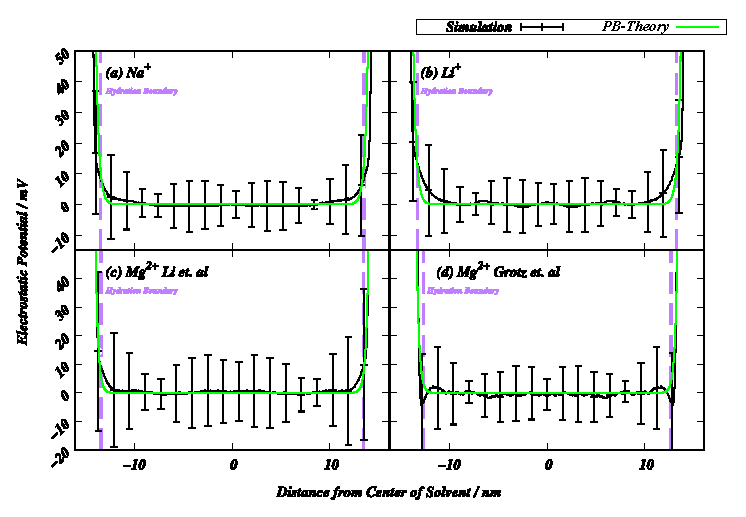
\includegraphics[height=0.5\textheight]{Figure_6.eps}
\end{figure}
\section{Conclusions}
We have presented a comparison between
two \mg{} parameter sets developed by our
group, under two different water–ion
interaction models. The \mg{ 2024}
parameters, optimized using clusters of
ions and lipid-component ligands at
sub-full oxygen coordination of the
ion~\cite{saunders:2024}, predict steric
adsorption with negligible bilayer
thickening. By contrast, the \mg{ 2025}
parameters, optimized using fully
coordinated clusters by replacing the
missing ligand oxygens with
waters, similar to sets of target data used to improve parameters for \mg{-nucleotide} phosphate interactions~\cite{julian:2023:mg}, yield
significantly more ions in non-steric
adsorption modes, greater direct
coordination with lipid phosphates, and a
correlated increase in bilayer thickness.
Both parameter sets reproduce their
respective substitution energy targets,
but the choice of partially versus fully
coordinated clusters leads to divergent
predictions for bilayer behavior.
 This raises a fundamental question about the nature of
\mg{} adsorption, and potentially of
divalent ions in general. Both
water-separated and direct-interaction
adsorption modes have been described for
\mg{}–phosphate interactions in biological
molecules~\cite{grotz:thesis,micro,grotz:2021:optimized,
villaparams,dudev:2003,rulivsek:2003:outer,
porschke:1979:mode,bowman:2012,fingerhut:2021:contact},
and simulations with older ion models tend
to favor the water-separated
modes~\cite{grotz:thesis,micro,grotz:2021:optimized,
villaparams,puyo:2022:consistent}. With
sparse experimental data for lipid bilayers
at relevant salt concentrations, it is not
yet possible to judge between these models.
Thus, the two parameter sets serve as
complementary hypotheses and experimental
targets, highlighting that the critical open
question is not only which parameters best
reproduce bilayer structure, but also which
underlying reference chemistry most
faithfully represents \mg{–lipid}
interactions in the condensed phase.

\FloatBarrier

\chapter{Conclusions}
\graphicspath{{CH5/figures/}}
\TODO{
We have introduced a framework for classifying ion adsorption at lipid bilayers based on the degree of dehydration observed in molecular dynamics simulations. This classification distinguishes between steric, imperfect, and perfect adsorption modes, corresponding to fully hydrated, partially dehydrated, and completely dehydrated ions within the hydration boundary of the bilayer.

Our results show that the electric field at the hydration shell of an ion correlates strongly with its observed mode of adsorption. Ions with high field strength, such as \mg, remain hydrated and adsorb sterically. In contrast, \na\ and \li\ exhibit lower field strengths and bind with partial or full dehydration.

These adsorption modes are predictive of changes to bilayer structure. Systems with larger populations of imperfect or perfectly adsorbed ions display increased lipid chain order and hydrocarbon thickness. Systems dominated by steric adsorption show bilayer structures closer to the no-salt case.

The observed trends hold across multiple force-field parameterizations, including those with differing water-exchange kinetics for \mg. Poisson--Boltzmann modeling confirms that the accumulation of ions within the hydration boundary is distinct from diffuse ionic layering predicted in the bulk.

Altogether, this work provides a mechanistic link between ion properties and lipid structural response, grounded in simulation observables. It suggests that the strength of ion adsorption---and its structural consequences---can be anticipated from the ion's electric field without requiring direct tuning to experimental constraints.
}
\bibliography{refs}
\end{document}




\begingroup
\clubpenalty=10000
\widowpenalty=10000
\interlinepenalty=10000
\sloppy
\bibliography{refs}
\endgroup
%----------------------------------------------------------
% Appendices
%----------------------------------------------------------
\appendix
\chapter{Appendices}
\section{Copyright Information and Author Contributions}
\label{app:permissions}
This appendix contains publisher permission agreements for reuse of material
from Chapters~2–4, and author contributions for each included article.



% Chapter 2 permissions
\subsection{Matthew Saunders, Vered Wineman-Fisher, and Eric Jakobsson, \textit{High-Dimensional Parameter Search Method to Determine Force Field Mixing Terms in Molecular Simulations}, 
\textit{Langmuir}, American Chemical Society, March 1, 2022}
\label{app:permissions1}
In this work I created geometries for target data, performed calculations for classical force-field target data.
I set up and performed parameter searches, implemented the force-field parameters, and ran all classical molecular dynamics simulations.
I performed all analysis and generated all figures, and wrote 90\% of the manuscript text.
\includepdf[
  pages={1-4},
  nup=2x2,
  frame=true,
  scale=0.8,
  pagecommand={}
]{Permissionforreuse1.pdf}

% Chapter 3 permissions
\subsection{Matthew Saunders, Abibat Adekeye-Olowofela, and Sabrina Downing, \textit{Adsorption Modes of Na\textsuperscript{+}, Li\textsuperscript{+}, and Mg\textsuperscript{2+} to a Model Zwitterionic Lipid Bilayer}, 
\textit{Langmuir}, American Chemical Society, December 1, 2024}
\label{app:permissions2}
In this work I created geometries for target data, performed both \emph{ab initio} and 
classical calculations for the target data.
I set up and performed parameter searches, implemented the force-field parameters, and ran all classical molecular dynamics simulations.
I performed all analysis and generated all figures, and wrote the manuscript text.
\includepdf[
  pages={1-4},
  nup=2x2,
  frame=true,
  scale=0.8,
  pagecommand={}
]{Permissionforreuse2.pdf}

% Chapter 4 permissions
\subsection{Matthew Saunders; Sagar A. Pandit; Sameer Varma.
Alteration of Lipid Bilayer Structure by Mg$^{2+}$.
\textit{Langmuir}, American Chemical Society, manuscript in review, 2025.}
\label{app:permissions3}
In this work I created geometries for target data, performed both \emph{ab initio} and 
classical calculations for the target data.
I set up and performed parameter searches, implemented the force-field parameters, and ran all classical molecular dynamics simulations.
I performed all analysis and generated all figures, and wrote the manuscript text.
% \includepdf[
%   pages=-,
%   pagecommand={},
%   scale=0.95
% ]{Permissionforreuse3.pdf}



\end{document}


